\documentclass[a4paper,11pt]{article}
\usepackage[a4paper, margin=8em]{geometry}

% usa i pacchetti per la scrittura in italiano
\usepackage[french,italian]{babel}
\usepackage[T1]{fontenc}
\usepackage[utf8]{inputenc}
\frenchspacing 

% usa i pacchetti per la formattazione matematica
\usepackage{amsmath, amssymb, amsthm, amsfonts}

% usa altri pacchetti
\usepackage{gensymb}
\usepackage{hyperref}
\usepackage{standalone}

\usepackage{colortbl}

\usepackage{xstring}
\usepackage{karnaugh-map}

% imposta il titolo
\title{Appunti Reti Informatiche}
\author{Luca Seggiani}
\date{2025}

% imposta lo stile
% usa helvetica
\usepackage[scaled]{helvet}
% usa palatino
\usepackage{palatino}
% usa un font monospazio guardabile
\usepackage{lmodern}

\renewcommand{\rmdefault}{ppl}
\renewcommand{\sfdefault}{phv}
\renewcommand{\ttdefault}{lmtt}

% circuiti
\usepackage{circuitikz}
\usetikzlibrary{babel}

% testo cerchiato
\newcommand*\circled[1]{\tikz[baseline=(char.base)]{
            \node[shape=circle,draw,inner sep=2pt] (char) {#1};}}

% disponi il titolo
\makeatletter
\renewcommand{\maketitle} {
	\begin{center} 
		\begin{minipage}[t]{.8\textwidth}
			\textsf{\huge\bfseries \@title} 
		\end{minipage}%
		\begin{minipage}[t]{.2\textwidth}
			\raggedleft \vspace{-1.65em}
			\textsf{\small \@author} \vfill
			\textsf{\small \@date}
		\end{minipage}
		\par
	\end{center}

	\thispagestyle{empty}
	\pagestyle{fancy}
}
\makeatother

% disponi teoremi
\usepackage{tcolorbox}
\newtcolorbox[auto counter, number within=section]{theorem}[2][]{%
	colback=blue!10, 
	colframe=blue!40!black, 
	sharp corners=northwest,
	fonttitle=\sffamily\bfseries, 
	title=Teorema~\thetcbcounter: #2, 
	#1
}

% disponi definizioni
\newtcolorbox[auto counter, number within=section]{definition}[2][]{%
	colback=red!10,
	colframe=red!40!black,
	sharp corners=northwest,
	fonttitle=\sffamily\bfseries,
	title=Definizione~\thetcbcounter: #2,
	#1
}

% disponi codice
\usepackage{listings}
\usepackage[table]{xcolor}

\definecolor{codegreen}{rgb}{0,0.6,0}
\definecolor{codegray}{rgb}{0.5,0.5,0.5}
\definecolor{codepurple}{rgb}{0.58,0,0.82}
\definecolor{backcolour}{rgb}{0.95,0.95,0.92}

\lstdefinestyle{codestyle}{
		backgroundcolor=\color{black!5}, 
		commentstyle=\color{codegreen},
		keywordstyle=\bfseries\color{magenta},
		numberstyle=\sffamily\tiny\color{black!60},
		stringstyle=\color{green!50!black},
		basicstyle=\ttfamily\footnotesize,
		breakatwhitespace=false,         
		breaklines=true,                 
		captionpos=b,                    
		keepspaces=true,                 
		numbers=left,                    
		numbersep=5pt,                  
		showspaces=false,                
		showstringspaces=false,
		showtabs=false,                  
		tabsize=2
}

\lstdefinestyle{shellstyle}{
		backgroundcolor=\color{black!5}, 
		basicstyle=\ttfamily\footnotesize\color{black}, 
		commentstyle=\color{black}, 
		keywordstyle=\color{black},
		numberstyle=\color{black!5},
		stringstyle=\color{black}, 
		showspaces=false,
		showstringspaces=false, 
		showtabs=false, 
		tabsize=2, 
		numbers=none, 
		breaklines=true
}


\lstdefinelanguage{assembler}{ 
  keywords={AAA, AAD, AAM, AAS, ADC, ADCB, ADCW, ADCL, ADD, ADDB, ADDW, ADDL, AND, ANDB, ANDW, ANDL,
        ARPL, BOUND, BSF, BSFL, BSFW, BSR, BSRL, BSRW, BSWAP, BT, BTC, BTCB, BTCW, BTCL, BTR, 
        BTRB, BTRW, BTRL, BTS, BTSB, BTSW, BTSL, CALL, CBW, CDQ, CLC, CLD, CLI, CLTS, CMC, CMP,
        CMPB, CMPW, CMPL, CMPS, CMPSB, CMPSD, CMPSW, CMPXCHG, CMPXCHGB, CMPXCHGW, CMPXCHGL,
        CMPXCHG8B, CPUID, CWDE, DAA, DAS, DEC, DECB, DECW, DECL, DIV, DIVB, DIVW, DIVL, ENTER,
        HLT, IDIV, IDIVB, IDIVW, IDIVL, IMUL, IMULB, IMULW, IMULL, IN, INB, INW, INL, INC, INCB,
        INCW, INCL, INS, INSB, INSD, INSW, INT, INT3, INTO, INVD, INVLPG, IRET, IRETD, JA, JAE,
        JB, JBE, JC, JCXZ, JE, JECXZ, JG, JGE, JL, JLE, JMP, JNA, JNAE, JNB, JNBE, JNC, JNE, JNG,
        JNGE, JNL, JNLE, JNO, JNP, JNS, JNZ, JO, JP, JPE, JPO, JS, JZ, LAHF, LAR, LCALL, LDS,
        LEA, LEAVE, LES, LFS, LGDT, LGS, LIDT, LMSW, LOCK, LODSB, LODSD, LODSW, LOOP, LOOPE,
        LOOPNE, LSL, LSS, LTR, MOV, MOVB, MOVW, MOVL, MOVSB, MOVSD, MOVSW, MOVSX, MOVSXB,
        MOVSXW, MOVSXL, MOVZX, MOVZXB, MOVZXW, MOVZXL, MUL, MULB, MULW, MULL, NEG, NEGB, NEGW,
        NEGL, NOP, NOT, NOTB, NOTW, NOTL, OR, ORB, ORW, ORL, OUT, OUTB, OUTW, OUTL, OUTSB, OUTSD,
        OUTSW, POP, POPL, POPW, POPB, POPA, POPAD, POPF, POPFD, PUSH, PUSHL, PUSHW, PUSHB, PUSHA, 
				PUSHAD, PUSHF, PUSHFD, RCL, RCLB, RCLW, MOVSL, MOVSB, MOVSW, STOSL, STOSB, STOSW, LODSB, LODSW,
				LODSL, INSB, INSW, INSL, OUTSB, OUTSL, OUTSW
        RCLL, RCR, RCRB, RCRW, RCRL, RDMSR, RDPMC, RDTSC, REP, REPE, REPNE, RET, ROL, ROLB, ROLW,
        ROLL, ROR, RORB, RORW, RORL, SAHF, SAL, SALB, SALW, SALL, SAR, SARB, SARW, SARL, SBB,
        SBBB, SBBW, SBBL, SCASB, SCASD, SCASW, SETA, SETAE, SETB, SETBE, SETC, SETE, SETG, SETGE,
        SETL, SETLE, SETNA, SETNAE, SETNB, SETNBE, SETNC, SETNE, SETNG, SETNGE, SETNL, SETNLE,
        SETNO, SETNP, SETNS, SETNZ, SETO, SETP, SETPE, SETPO, SETS, SETZ, SGDT, SHL, SHLB, SHLW,
        SHLL, SHLD, SHR, SHRB, SHRW, SHRL, SHRD, SIDT, SLDT, SMSW, STC, STD, STI, STOSB, STOSD,
        STOSW, STR, SUB, SUBB, SUBW, SUBL, TEST, TESTB, TESTW, TESTL, VERR, VERW, WAIT, WBINVD,
        XADD, XADDB, XADDW, XADDL, XCHG, XCHGB, XCHGW, XCHGL, XLAT, XLATB, XOR, XORB, XORW, XORL},
  keywordstyle=\color{blue}\bfseries,
  ndkeywordstyle=\color{darkgray}\bfseries,
  identifierstyle=\color{black},
  sensitive=false,
  comment=[l]{\#},
  morecomment=[s]{/*}{*/},
  commentstyle=\color{purple}\ttfamily,
  stringstyle=\color{red}\ttfamily,
  morestring=[b]',
  morestring=[b]"
}

\lstset{language=assembler, style=codestyle}

% disponi sezioni
\usepackage{titlesec}

\titleformat{\section}
	{\sffamily\Large\bfseries} 
	{\thesection}{1em}{} 
\titleformat{\subsection}
	{\sffamily\large\bfseries}   
	{\thesubsection}{1em}{} 
\titleformat{\subsubsection}
	{\sffamily\normalsize\bfseries} 
	{\thesubsubsection}{1em}{}

% tikz
\usepackage{tikz}

% float
\usepackage{float}

% grafici
\usepackage{pgfplots}
\pgfplotsset{width=10cm,compat=1.9}

% disponi alberi
\usepackage{forest}

\forestset{
	rectstyle/.style={
		for tree={rectangle,draw,font=\large\sffamily}
	},
	roundstyle/.style={
		for tree={circle,draw,font=\large}
	}
}

% disponi algoritmi
\usepackage{algorithm}
\usepackage{algorithmic}
\makeatletter
\renewcommand{\ALG@name}{Algoritmo}
\makeatother

% disponi numeri di pagina
\usepackage{fancyhdr}
\fancyhf{} 
\fancyfoot[L]{\sffamily{\thepage}}

\makeatletter
\fancyhead[L]{\raisebox{1ex}[0pt][0pt]{\sffamily{\@title \ \@date}}} 
\fancyhead[R]{\raisebox{1ex}[0pt][0pt]{\sffamily{\@author}}}
\makeatother

\begin{document}

\pagestyle{fancy}
\thispagestyle{empty}
\renewcommand{\thispagestyle}[1]{}

\maketitle
\documentclass[a4paper,11pt]{article}
\usepackage[a4paper, margin=8em]{geometry}

% usa i pacchetti per la scrittura in italiano
\usepackage[french,italian]{babel}
\usepackage[T1]{fontenc}
\usepackage[utf8]{inputenc}
\frenchspacing 

% usa i pacchetti per la formattazione matematica
\usepackage{amsmath, amssymb, amsthm, amsfonts}

% usa altri pacchetti
\usepackage{gensymb}
\usepackage{hyperref}
\usepackage{standalone}

\usepackage{colortbl}

\usepackage{xstring}
\usepackage{karnaugh-map}

% imposta il titolo
\title{Appunti Reti Informatiche}
\author{Luca Seggiani}
\date{2025}

% imposta lo stile
% usa helvetica
\usepackage[scaled]{helvet}
% usa palatino
\usepackage{palatino}
% usa un font monospazio guardabile
\usepackage{lmodern}

\renewcommand{\rmdefault}{ppl}
\renewcommand{\sfdefault}{phv}
\renewcommand{\ttdefault}{lmtt}

% circuiti
\usepackage{circuitikz}
\usetikzlibrary{babel}

% testo cerchiato
\newcommand*\circled[1]{\tikz[baseline=(char.base)]{
            \node[shape=circle,draw,inner sep=2pt] (char) {#1};}}

% disponi il titolo
\makeatletter
\renewcommand{\maketitle} {
	\begin{center} 
		\begin{minipage}[t]{.8\textwidth}
			\textsf{\huge\bfseries \@title} 
		\end{minipage}%
		\begin{minipage}[t]{.2\textwidth}
			\raggedleft \vspace{-1.65em}
			\textsf{\small \@author} \vfill
			\textsf{\small \@date}
		\end{minipage}
		\par
	\end{center}

	\thispagestyle{empty}
	\pagestyle{fancy}
}
\makeatother

% disponi teoremi
\usepackage{tcolorbox}
\newtcolorbox[auto counter, number within=section]{theorem}[2][]{%
	colback=blue!10, 
	colframe=blue!40!black, 
	sharp corners=northwest,
	fonttitle=\sffamily\bfseries, 
	title=Teorema~\thetcbcounter: #2, 
	#1
}

% disponi definizioni
\newtcolorbox[auto counter, number within=section]{definition}[2][]{%
	colback=red!10,
	colframe=red!40!black,
	sharp corners=northwest,
	fonttitle=\sffamily\bfseries,
	title=Definizione~\thetcbcounter: #2,
	#1
}

% disponi codice
\usepackage{listings}
\usepackage[table]{xcolor}

\definecolor{codegreen}{rgb}{0,0.6,0}
\definecolor{codegray}{rgb}{0.5,0.5,0.5}
\definecolor{codepurple}{rgb}{0.58,0,0.82}
\definecolor{backcolour}{rgb}{0.95,0.95,0.92}

\lstdefinestyle{codestyle}{
		backgroundcolor=\color{black!5}, 
		commentstyle=\color{codegreen},
		keywordstyle=\bfseries\color{magenta},
		numberstyle=\sffamily\tiny\color{black!60},
		stringstyle=\color{green!50!black},
		basicstyle=\ttfamily\footnotesize,
		breakatwhitespace=false,         
		breaklines=true,                 
		captionpos=b,                    
		keepspaces=true,                 
		numbers=left,                    
		numbersep=5pt,                  
		showspaces=false,                
		showstringspaces=false,
		showtabs=false,                  
		tabsize=2
}

\lstdefinestyle{shellstyle}{
		backgroundcolor=\color{black!5}, 
		basicstyle=\ttfamily\footnotesize\color{black}, 
		commentstyle=\color{black}, 
		keywordstyle=\color{black},
		numberstyle=\color{black!5},
		stringstyle=\color{black}, 
		showspaces=false,
		showstringspaces=false, 
		showtabs=false, 
		tabsize=2, 
		numbers=none, 
		breaklines=true
}


\lstdefinelanguage{assembler}{ 
  keywords={AAA, AAD, AAM, AAS, ADC, ADCB, ADCW, ADCL, ADD, ADDB, ADDW, ADDL, AND, ANDB, ANDW, ANDL,
        ARPL, BOUND, BSF, BSFL, BSFW, BSR, BSRL, BSRW, BSWAP, BT, BTC, BTCB, BTCW, BTCL, BTR, 
        BTRB, BTRW, BTRL, BTS, BTSB, BTSW, BTSL, CALL, CBW, CDQ, CLC, CLD, CLI, CLTS, CMC, CMP,
        CMPB, CMPW, CMPL, CMPS, CMPSB, CMPSD, CMPSW, CMPXCHG, CMPXCHGB, CMPXCHGW, CMPXCHGL,
        CMPXCHG8B, CPUID, CWDE, DAA, DAS, DEC, DECB, DECW, DECL, DIV, DIVB, DIVW, DIVL, ENTER,
        HLT, IDIV, IDIVB, IDIVW, IDIVL, IMUL, IMULB, IMULW, IMULL, IN, INB, INW, INL, INC, INCB,
        INCW, INCL, INS, INSB, INSD, INSW, INT, INT3, INTO, INVD, INVLPG, IRET, IRETD, JA, JAE,
        JB, JBE, JC, JCXZ, JE, JECXZ, JG, JGE, JL, JLE, JMP, JNA, JNAE, JNB, JNBE, JNC, JNE, JNG,
        JNGE, JNL, JNLE, JNO, JNP, JNS, JNZ, JO, JP, JPE, JPO, JS, JZ, LAHF, LAR, LCALL, LDS,
        LEA, LEAVE, LES, LFS, LGDT, LGS, LIDT, LMSW, LOCK, LODSB, LODSD, LODSW, LOOP, LOOPE,
        LOOPNE, LSL, LSS, LTR, MOV, MOVB, MOVW, MOVL, MOVSB, MOVSD, MOVSW, MOVSX, MOVSXB,
        MOVSXW, MOVSXL, MOVZX, MOVZXB, MOVZXW, MOVZXL, MUL, MULB, MULW, MULL, NEG, NEGB, NEGW,
        NEGL, NOP, NOT, NOTB, NOTW, NOTL, OR, ORB, ORW, ORL, OUT, OUTB, OUTW, OUTL, OUTSB, OUTSD,
        OUTSW, POP, POPL, POPW, POPB, POPA, POPAD, POPF, POPFD, PUSH, PUSHL, PUSHW, PUSHB, PUSHA, 
				PUSHAD, PUSHF, PUSHFD, RCL, RCLB, RCLW, MOVSL, MOVSB, MOVSW, STOSL, STOSB, STOSW, LODSB, LODSW,
				LODSL, INSB, INSW, INSL, OUTSB, OUTSL, OUTSW
        RCLL, RCR, RCRB, RCRW, RCRL, RDMSR, RDPMC, RDTSC, REP, REPE, REPNE, RET, ROL, ROLB, ROLW,
        ROLL, ROR, RORB, RORW, RORL, SAHF, SAL, SALB, SALW, SALL, SAR, SARB, SARW, SARL, SBB,
        SBBB, SBBW, SBBL, SCASB, SCASD, SCASW, SETA, SETAE, SETB, SETBE, SETC, SETE, SETG, SETGE,
        SETL, SETLE, SETNA, SETNAE, SETNB, SETNBE, SETNC, SETNE, SETNG, SETNGE, SETNL, SETNLE,
        SETNO, SETNP, SETNS, SETNZ, SETO, SETP, SETPE, SETPO, SETS, SETZ, SGDT, SHL, SHLB, SHLW,
        SHLL, SHLD, SHR, SHRB, SHRW, SHRL, SHRD, SIDT, SLDT, SMSW, STC, STD, STI, STOSB, STOSD,
        STOSW, STR, SUB, SUBB, SUBW, SUBL, TEST, TESTB, TESTW, TESTL, VERR, VERW, WAIT, WBINVD,
        XADD, XADDB, XADDW, XADDL, XCHG, XCHGB, XCHGW, XCHGL, XLAT, XLATB, XOR, XORB, XORW, XORL},
  keywordstyle=\color{blue}\bfseries,
  ndkeywordstyle=\color{darkgray}\bfseries,
  identifierstyle=\color{black},
  sensitive=false,
  comment=[l]{\#},
  morecomment=[s]{/*}{*/},
  commentstyle=\color{purple}\ttfamily,
  stringstyle=\color{red}\ttfamily,
  morestring=[b]',
  morestring=[b]"
}

\lstset{language=assembler, style=codestyle}

% disponi sezioni
\usepackage{titlesec}

\titleformat{\section}
	{\sffamily\Large\bfseries} 
	{\thesection}{1em}{} 
\titleformat{\subsection}
	{\sffamily\large\bfseries}   
	{\thesubsection}{1em}{} 
\titleformat{\subsubsection}
	{\sffamily\normalsize\bfseries} 
	{\thesubsubsection}{1em}{}

% tikz
\usepackage{tikz}

% float
\usepackage{float}

% grafici
\usepackage{pgfplots}
\pgfplotsset{width=10cm,compat=1.9}

% disponi alberi
\usepackage{forest}

\forestset{
	rectstyle/.style={
		for tree={rectangle,draw,font=\large\sffamily}
	},
	roundstyle/.style={
		for tree={circle,draw,font=\large}
	}
}

% disponi algoritmi
\usepackage{algorithm}
\usepackage{algorithmic}
\makeatletter
\renewcommand{\ALG@name}{Algoritmo}
\makeatother

% disponi numeri di pagina
\usepackage{fancyhdr}
\fancyhf{} 
\fancyfoot[L]{\sffamily{\thepage}}

\makeatletter
\fancyhead[L]{\raisebox{1ex}[0pt][0pt]{\sffamily{\@title \ \@date}}} 
\fancyhead[R]{\raisebox{1ex}[0pt][0pt]{\sffamily{\@author}}}
\makeatother

\begin{document}
% sezione (data)
\section{Lezione del 23-09-25}

% stili pagina
\thispagestyle{empty}
\pagestyle{fancy}

% testo
\subsection{Introduzione}
Il corso si pone di presentare le nozioni di base sulle reti informatiche, le tecnologie di rete più diffuse, i protocolli Internet e lo sviluppo di applicazioni distribuite \textit{client-server} e \textit{peer-to-peer} (\textbf{P2P}).

In particolare il programma del corso comprende:
\begin{itemize}
	\item Sviluppo di \textbf{applicazioni} in rete:
		\begin{itemize}
			\item Client-server;
			\item Peer-to-peer.
		\end{itemize}
	\item Reti a \textbf{connessione diretta}:
		\begin{itemize}
			\item Collegamenti punto-punto;
			\item Reti locali.
		\end{itemize}
	\item Reti a \textbf{commutazione di pacchetto};
	\item \textbf{Interconnessione} di reti di tipo diverso;
	\item \textbf{Trasporto} end-to-end e protocolli;
	\item \textbf{Sicurezza};
	\item Reti \textbf{wireless} e \textbf{mobili}, intese come caso particolare delle normali reti \textbf{cablate} (\textit{wired}).
\end{itemize}

\subsubsection{Applicazioni in rete}
Nel dettaglio delle \textit{applicazioni in rete}, vedremo come già detto i paradigmi \textit{client-server} e \textit{peer-to-peer}, di cui possiamo già fare alcuni esempi:
\begin{itemize}
	\item Applicazioni client-server:
		\begin{itemize}
			\item Web;
			\item Trasferimento file;
			\item Posta elettronica;
			\item DNS;
			\item Ecc...
		\end{itemize}
	\item Applicazioni peer-to-peer:
		\begin{itemize}
			\item Ricerca di contenuti;
			\item Torrent;
			\item Telefonia online;
			\item Ecc...
		\end{itemize}
\end{itemize}

In questo ci avvarremo del concetto di \textbf{socket} come primitiva per la gestione della rete dal lato S/O.

\subsubsection{Reti dirette, a commutazione e wireless}
Inizieremo con lo studio di \textit{collegamenti punto-punto}, e quindi di trasferimento affidabile di dati fra 2 punti.
Vedremo poi le reti locali, ad accesso multiplo, e i casi particolari come \textit{Ethernet}.

Vedremo quindi le reti a \textit{commutazione di pacchetto} per la copertura di grandi regioni. Anche qui approfondiremo tecnologie come gli \textit{switch}, ancora \textit{Ethernet}, ecc...

Per quanto riguarda l'\textit{interconnessione di reti} vedremo il protocollo Internet \textbf{IPv4}, il \textbf{routing} (cioè l'\textit{instradamento}) e i protocolli di trasporto (\textbf{UDP} e \textbf{TCP}).

Parleremo anche di reti \textit{wireless} e \textit{mobili}, e quindi di tecnologie come \textbf{WiFi}, le \textbf{reti cellulari}, e reti senza infrastruttura come \textbf{Bluetooth}.

\subsubsection{Sicurezza}
Vedremo poi le minacce alla \textit{sicurezza} e alcune soluzioni che abbiamo a disposizione per mitigarle.
In particolare, tratteremo di \textbf{crittografia} e \textbf{integrità} dei messaggi. 

Nello specifico parleremo di tecnologie a livello applicazione (\textbf{PGP}), a livello trasporto (\textbf{TLS} (usata in \textit{HTTPS})), a livello Internet (\textbf{IP-Sec}) e difese di sicurezza come \textbf{firewall} e \textbf{IDS}.

\subsection{Terminologia}
Iniziamo quindi a definire la terminologia di base usata nel corso, usando Internet come esempio.

\subsubsection{Internet}
La prima domanda che ci poniamo è \textit{"Che cos'è Internet?"}.

\par\medskip
\textbf{\textsf{Visione ingegneristica}} \\
\noindent
Iniziamo col vedere la definizione di Internet agli occhi di un ingegnere che si occupa di reti: 
\begin{itemize}
	\item Si tratterà di una rete che connette miliardi di \textit{dispositivi}, detti \textbf{host} (\textit{"ospiti"}), che eseguono \textit{applicazioni in rete} al cosiddetto \textbf{edge} (\textit{"bordo"}) della rete.
	\item Una visione \textbf{interna} della rete ci dirà invece che è un insieme di \textbf{pacchetti} che viaggiano attraverso infrastruttura (\textit{router}, \textit{switch}), per raggiungere il loro destinatario.
	\item A livello \textbf{fisico} potremmo considerare le connessioni fisiche fra dispositivi, date da cavi, segnali radio, ecc...
	\item Infine, potremo organizzare le \textbf{reti} come collezioni di dispositivi, router e connessioni gestite da determinate organizzazioni.
\end{itemize}

Non è esattamente corretto parlare di \textit{"reti di calcolatori"} in quanto oggi ad essere connessi a Internet sono tutta una gamma di dispositivi non necessariamente orientati al puro \textit{calcolo}: è questo il caso del cosiddetto \textit{Internet of Things} (\textbf{IoT}).

\par\medskip

Possiamo quindi intendere Internet come una "rete di reti", cioè più \textbf{ISP} (\textit{Internet Service Providers}) connessi fra di loro, che a loro volta connettono una gamma dispositivi (host, router, switch, ecc...).

Per governare l'operazione di tali rete si necessita di \textbf{protocolli}, che definiscono il modo in cui si inviano e ricevono messaggi in rete.

In particolare, per quanto riguarda Internet notiamo l'\textbf{IETF} (\textit{Internet Engineering Task Force}), organizzazione che gestisce diversi standard del settore (anche detti \textbf{RFC}, da \textit{Request For Comments memoranda}).

\par\medskip
\textbf{\textsf{Visione utente}} \\
\noindent
Per l'utente, internet sarà un insieme di \textbf{infrastrutture} che forniscono \textbf{servizi} finali, fra cui il Web, telecomunicazioni, streaming, ecc...
Dal punto di vista delle \textbf{applicazioni} in esecuzione sui dispositivi, Internet rappresenterà un'interfaccia di programmazione per consentire la comunicazione fra processi su una o più macchine.
In questo parleremo di \textbf{hook} che permettono alle applicazioni di \textbf{connettersi} a Internet, cioè accedere ad un qualche protocollo di trasporto dei dati. 

\subsubsection{Protocolli}
Un \textbf{protocollo} è una precisa \textit{specifica} del formato secondo il quale due dispositivi in rete si scambiano informazioni.
Solitamente i protocolli si sviluppano in più fasi, successive nel tempo, dove si portano avanti diverse operazioni necessarie alla comunicazione.

Esempi di protocollo sono il \textit{protocollo Internet} \textbf{IPv4}, e il \textit{protocollo di trasporto} \textbf{TCP} usato nel \textit{Web} e visto nel corso di progettazione web.

\subsubsection{Infrastruttura di Internet}
Vediamo più nel dettaglio la struttura di Internet:
\begin{itemize}
	\item 
	Abbiamo detto che all'\textit{edge} di internet ci sono i cosiddetti \textit{host}, cioè i \textbf{client} e i \textbf{server}. Notiamo che non vogliamo riferirci alle macchine fisiche client o server, ma ai \textbf{processi} che si comportano come tali per l'implementazione di un'applicazione distribuita.
	\item
	I dispositivi \textit{terminali} che abbiamo appena nominato accedono ad Internet attraverso le cosiddette \textbf{reti di accesso}, cablate o wireless e basate sulle tecnologie utilizzate (router).

	Per collegare i sistemi terminali ai router si usano \textit{reti residenziali}, \textit{reti di accesso istituzionali} (scuola, lavoro, ecc...), nonché \textit{reti wireless e mobili} (Wifi, o reti come 4G solitamente fornite da privati).
	In questo caso può interessarci la frequenza di trasmissione, in bit al secondo, di una rete di accesso, o se quella rete è ad accesso \textit{condiviso} (pensa WiFi) o \textit{dedicato} (pensa Ethernet).

	Uno standard storico per le reti di accesso è quello della trasmissione sulla linea telefonica su \textbf{DSL} (\textit{Digital Subscriber Line}).
	Negli Stati Uniti si è invece diffuso l'uso dela linea televisiva cablata.
	Oggi, sfruttiamo invece tecnologie come \textbf{ADSL} (\textit{Asymmetric Digital Subscriber Line}) e \textbf{FTTC} (\textit{Fiber To The Cabinet}).
	La differenza principale fra queste è che la linea in ADSL è interamente in rame, sia dalla centrale all'armadio di ripartizione che dall'armadio ripartilinea agli utenti finali, mentre nella linea FTTC si porta il segnale all'armadio attraverso cavi in fibra ottica.
	Lo standard di ultima generazione è \textbf{FTTH} (\textit{Fiber To The Home}), che prevede una linea in fibra ottica anche dall'armadio agli utenti finali.

	Possiamo quindi vedere la rete locale (\textbf{LAN} (\textit{Local Area Network})) di una comune abitazione come composta da un router, connesso a un \textbf{modem} DSL (\textit{modem} deriva da modulatore/demodulatore sulla linea telefonica dei messaggi Internet) o direttamente via cavo ad un altro centro di ripartizione, e ad eventuali dispositivi come \textit{access point WiFi} che offrono la connessione via rete mobile ai dispositivi finali (una cosiddetta \textbf{WLAN}, \textit{Wireless Local Area Network}).

	Altre soluzioni per le comunicazioni wireless sono rappresentati da reti \textbf{cellulari} su larga scala, che sono quelle usate dagli operatori telefonici (tecnologie come \textbf{4G}, ecc...).

	\item 
	Dalle reti di accesso si arriva a Internet attraverso reti interconnesse di router, arrivando quindi alle \textit{reti di reti} di cui stavamo parlando.
\end{itemize}


\end{document}

\documentclass[a4paper,11pt]{article}
\usepackage[a4paper, margin=8em]{geometry}

% usa i pacchetti per la scrittura in italiano
\usepackage[french,italian]{babel}
\usepackage[T1]{fontenc}
\usepackage[utf8]{inputenc}
\frenchspacing 

% usa i pacchetti per la formattazione matematica
\usepackage{amsmath, amssymb, amsthm, amsfonts}

% usa altri pacchetti
\usepackage{gensymb}
\usepackage{hyperref}
\usepackage{standalone}

\usepackage{colortbl}

\usepackage{xstring}
\usepackage{karnaugh-map}

% imposta il titolo
\title{Appunti Reti Informatiche}
\author{Luca Seggiani}
\date{2025}

% imposta lo stile
% usa helvetica
\usepackage[scaled]{helvet}
% usa palatino
\usepackage{palatino}
% usa un font monospazio guardabile
\usepackage{lmodern}

\renewcommand{\rmdefault}{ppl}
\renewcommand{\sfdefault}{phv}
\renewcommand{\ttdefault}{lmtt}

% circuiti
\usepackage{circuitikz}
\usetikzlibrary{babel}

% testo cerchiato
\newcommand*\circled[1]{\tikz[baseline=(char.base)]{
            \node[shape=circle,draw,inner sep=2pt] (char) {#1};}}

% disponi il titolo
\makeatletter
\renewcommand{\maketitle} {
	\begin{center} 
		\begin{minipage}[t]{.8\textwidth}
			\textsf{\huge\bfseries \@title} 
		\end{minipage}%
		\begin{minipage}[t]{.2\textwidth}
			\raggedleft \vspace{-1.65em}
			\textsf{\small \@author} \vfill
			\textsf{\small \@date}
		\end{minipage}
		\par
	\end{center}

	\thispagestyle{empty}
	\pagestyle{fancy}
}
\makeatother

% disponi teoremi
\usepackage{tcolorbox}
\newtcolorbox[auto counter, number within=section]{theorem}[2][]{%
	colback=blue!10, 
	colframe=blue!40!black, 
	sharp corners=northwest,
	fonttitle=\sffamily\bfseries, 
	title=Teorema~\thetcbcounter: #2, 
	#1
}

% disponi definizioni
\newtcolorbox[auto counter, number within=section]{definition}[2][]{%
	colback=red!10,
	colframe=red!40!black,
	sharp corners=northwest,
	fonttitle=\sffamily\bfseries,
	title=Definizione~\thetcbcounter: #2,
	#1
}

% disponi codice
\usepackage{listings}
\usepackage[table]{xcolor}

\definecolor{codegreen}{rgb}{0,0.6,0}
\definecolor{codegray}{rgb}{0.5,0.5,0.5}
\definecolor{codepurple}{rgb}{0.58,0,0.82}
\definecolor{backcolour}{rgb}{0.95,0.95,0.92}

\lstdefinestyle{codestyle}{
		backgroundcolor=\color{black!5}, 
		commentstyle=\color{codegreen},
		keywordstyle=\bfseries\color{magenta},
		numberstyle=\sffamily\tiny\color{black!60},
		stringstyle=\color{green!50!black},
		basicstyle=\ttfamily\footnotesize,
		breakatwhitespace=false,         
		breaklines=true,                 
		captionpos=b,                    
		keepspaces=true,                 
		numbers=left,                    
		numbersep=5pt,                  
		showspaces=false,                
		showstringspaces=false,
		showtabs=false,                  
		tabsize=2
}

\lstdefinestyle{shellstyle}{
		backgroundcolor=\color{black!5}, 
		basicstyle=\ttfamily\footnotesize\color{black}, 
		commentstyle=\color{black}, 
		keywordstyle=\color{black},
		numberstyle=\color{black!5},
		stringstyle=\color{black}, 
		showspaces=false,
		showstringspaces=false, 
		showtabs=false, 
		tabsize=2, 
		numbers=none, 
		breaklines=true
}


\lstdefinelanguage{assembler}{ 
  keywords={AAA, AAD, AAM, AAS, ADC, ADCB, ADCW, ADCL, ADD, ADDB, ADDW, ADDL, AND, ANDB, ANDW, ANDL,
        ARPL, BOUND, BSF, BSFL, BSFW, BSR, BSRL, BSRW, BSWAP, BT, BTC, BTCB, BTCW, BTCL, BTR, 
        BTRB, BTRW, BTRL, BTS, BTSB, BTSW, BTSL, CALL, CBW, CDQ, CLC, CLD, CLI, CLTS, CMC, CMP,
        CMPB, CMPW, CMPL, CMPS, CMPSB, CMPSD, CMPSW, CMPXCHG, CMPXCHGB, CMPXCHGW, CMPXCHGL,
        CMPXCHG8B, CPUID, CWDE, DAA, DAS, DEC, DECB, DECW, DECL, DIV, DIVB, DIVW, DIVL, ENTER,
        HLT, IDIV, IDIVB, IDIVW, IDIVL, IMUL, IMULB, IMULW, IMULL, IN, INB, INW, INL, INC, INCB,
        INCW, INCL, INS, INSB, INSD, INSW, INT, INT3, INTO, INVD, INVLPG, IRET, IRETD, JA, JAE,
        JB, JBE, JC, JCXZ, JE, JECXZ, JG, JGE, JL, JLE, JMP, JNA, JNAE, JNB, JNBE, JNC, JNE, JNG,
        JNGE, JNL, JNLE, JNO, JNP, JNS, JNZ, JO, JP, JPE, JPO, JS, JZ, LAHF, LAR, LCALL, LDS,
        LEA, LEAVE, LES, LFS, LGDT, LGS, LIDT, LMSW, LOCK, LODSB, LODSD, LODSW, LOOP, LOOPE,
        LOOPNE, LSL, LSS, LTR, MOV, MOVB, MOVW, MOVL, MOVSB, MOVSD, MOVSW, MOVSX, MOVSXB,
        MOVSXW, MOVSXL, MOVZX, MOVZXB, MOVZXW, MOVZXL, MUL, MULB, MULW, MULL, NEG, NEGB, NEGW,
        NEGL, NOP, NOT, NOTB, NOTW, NOTL, OR, ORB, ORW, ORL, OUT, OUTB, OUTW, OUTL, OUTSB, OUTSD,
        OUTSW, POP, POPL, POPW, POPB, POPA, POPAD, POPF, POPFD, PUSH, PUSHL, PUSHW, PUSHB, PUSHA, 
				PUSHAD, PUSHF, PUSHFD, RCL, RCLB, RCLW, MOVSL, MOVSB, MOVSW, STOSL, STOSB, STOSW, LODSB, LODSW,
				LODSL, INSB, INSW, INSL, OUTSB, OUTSL, OUTSW
        RCLL, RCR, RCRB, RCRW, RCRL, RDMSR, RDPMC, RDTSC, REP, REPE, REPNE, RET, ROL, ROLB, ROLW,
        ROLL, ROR, RORB, RORW, RORL, SAHF, SAL, SALB, SALW, SALL, SAR, SARB, SARW, SARL, SBB,
        SBBB, SBBW, SBBL, SCASB, SCASD, SCASW, SETA, SETAE, SETB, SETBE, SETC, SETE, SETG, SETGE,
        SETL, SETLE, SETNA, SETNAE, SETNB, SETNBE, SETNC, SETNE, SETNG, SETNGE, SETNL, SETNLE,
        SETNO, SETNP, SETNS, SETNZ, SETO, SETP, SETPE, SETPO, SETS, SETZ, SGDT, SHL, SHLB, SHLW,
        SHLL, SHLD, SHR, SHRB, SHRW, SHRL, SHRD, SIDT, SLDT, SMSW, STC, STD, STI, STOSB, STOSD,
        STOSW, STR, SUB, SUBB, SUBW, SUBL, TEST, TESTB, TESTW, TESTL, VERR, VERW, WAIT, WBINVD,
        XADD, XADDB, XADDW, XADDL, XCHG, XCHGB, XCHGW, XCHGL, XLAT, XLATB, XOR, XORB, XORW, XORL},
  keywordstyle=\color{blue}\bfseries,
  ndkeywordstyle=\color{darkgray}\bfseries,
  identifierstyle=\color{black},
  sensitive=false,
  comment=[l]{\#},
  morecomment=[s]{/*}{*/},
  commentstyle=\color{purple}\ttfamily,
  stringstyle=\color{red}\ttfamily,
  morestring=[b]',
  morestring=[b]"
}

\lstset{language=assembler, style=codestyle}

% disponi sezioni
\usepackage{titlesec}

\titleformat{\section}
	{\sffamily\Large\bfseries} 
	{\thesection}{1em}{} 
\titleformat{\subsection}
	{\sffamily\large\bfseries}   
	{\thesubsection}{1em}{} 
\titleformat{\subsubsection}
	{\sffamily\normalsize\bfseries} 
	{\thesubsubsection}{1em}{}

% tikz
\usepackage{tikz}

% float
\usepackage{float}

% grafici
\usepackage{pgfplots}
\pgfplotsset{width=10cm,compat=1.9}

% disponi alberi
\usepackage{forest}

\forestset{
	rectstyle/.style={
		for tree={rectangle,draw,font=\large\sffamily}
	},
	roundstyle/.style={
		for tree={circle,draw,font=\large}
	}
}

% disponi algoritmi
\usepackage{algorithm}
\usepackage{algorithmic}
\makeatletter
\renewcommand{\ALG@name}{Algoritmo}
\makeatother

% disponi numeri di pagina
\usepackage{fancyhdr}
\fancyhf{} 
\fancyfoot[L]{\sffamily{\thepage}}

\makeatletter
\fancyhead[L]{\raisebox{1ex}[0pt][0pt]{\sffamily{\@title \ \@date}}} 
\fancyhead[R]{\raisebox{1ex}[0pt][0pt]{\sffamily{\@author}}}
\makeatother

\begin{document}
% sezione (data)
\section{Lezione del 24-09-25}

% stili pagina
\thispagestyle{empty}
\pagestyle{fancy}

% testo
\subsection{Comunicazione dati su Internet}
Abbiamo visto la struttura a livello fisico della rete Internet.
Vediamo adesso i meccanismi secondo cui la trasmissione di dati avviene.
La rete Internet è una rete a \textbf{commutazione di pacchetto}, il compito degli host è di:
\begin{itemize}
	\item Ottenere messaggi dalle applicazioni;
	\item Dividere quei messaggi in frammenti più piccoli, detti \textbf{pacchetti}, di dimensione $L$ bit;
	\item Trasmettere quei pacchetti nella rete di accesso ad una \textit{frequenza di trasmissione} (o \textbf{bit-rate}) $R$.
\end{itemize}

Il tempo $T_{\text{packet}}$ necessario a trasmettere un pacchetto da $L$ bit su una linea da $R$ bit al secondo di bitrate sarà quindi semplicemente calcolato come:
$$
T_{\text{packet}} = \frac{L}{R}
$$

Il bitrate, detto anche frequenza di \textit{link}, dipende appunto dal \textbf{link} (o \textit{mezzo}) della trasmissione, cioè l'infrastruttura fisica che sta fra trasmettitore e ricevitore.
Possiamo classificare 2 tipi di link:
\begin{itemize}
	\item Mezzi \textbf{guidati}: segnali che si propagano in mezzi solidi (rame, fibra, cavi coassiali, ecc...). 

		\begin{itemize}
			\item 
		Un celebre esempio di mezzo trasmissivo guidato è il classico \textbf{doppino telefonico}, o trasmettitore a \textit{Twisted Pair} (\textbf{TP}). Questo è formato da due fili di rame isolati e avvolti l'uno sull'altro, che permettono la trasmissione differenziale e quindi la riduzione dei rumori in \textit{common-mode};
			\item
		Un altro tipo di mezzo trasmissivo guidato è il \textbf{cavo coassiale}, formato da due conduttori concentrici in rame separati da un dielettrico. Il segnale è trasferito come campo magnetico fra i due conduttori: questo permette bitrate più alti rispetto al normale doppino telefonico e una migliore schermatura dalle interferenze;
			\item
		Infine, possiamo parlare della \textbf{fibra ottica}, formata da fibra di vetro che porta impulsi luminosi ad altissima velocità. Questa tecnologia presenta velocità di trasmissione estremamente alte, e vista la natura luminosa del segnale, non è suscettibile ad interferenze (alta affidabilità, cioè piccola frequenza di errore sui bit).
		\end{itemize}

	\item Mezzi \textbf{non guidati}: segnali che si propagano nell'etere (segnali radio, ecc...). Questi sono solitamente meno sicuri ma significativamente più comodi per l'utente finale (possibilità di spostarsi, mancanza di cavi, ecc...).

		La trasmissione wireless è suscettibile a fenomeni fisici come \textit{riflessi}, \textit{interferenze} e \textit{ostruzione} da parte di oggetti fisici.

		\begin{itemize}
			\item Il \textbf{WiFi} è un esempio di mezzo di trasmissione non guidato che può raggiungere centinaia di Mbps su regioni locali;
			\item Reti wireless più ampie possono essere quelle \textbf{cellulari}, usate nella telefonia mobile;
			\item Infine si può parlare delle \textbf{reti satellitari}, usate per l'interconnessione di regioni geografiche fra di loro anche molto distanti.
		\end{itemize}

\end{itemize}

\subsubsection{Commutazione di circuito}
Prima della commutazione di pacchetto si usava la tecnica della \textbf{commutazione di circuito} (ad esempio sulle linee telefoniche).
Questo prevede di dedicare completamente una certa linea di trasmissione alla comunicazione fra due host, invalidandone quindi l'uso da parte di altri host.

Chiaramente, la commutazione di pacchetto permette un carico migliore della linea, dove più pacchetti provenienti da diverse fonti possono viaggiare a istanti temporali molto vicini fra di loro.

In particolare, la commutazione di paccheto è utile per dati trasmessi in \textit{burst}, mentre la rete a commutazione di circuito assicura minima congestione possibile a costo di occupazione completa della linea.

\subsubsection{Commutazione di pacchetto}
La tecnica della \textbf{commutazione di pacchetto} o \textit{packet-switching} permette ad una rete di \textbf{router} interconnessi di ricevere ed instradare (letteralmente, \textit{"routing"}) pacchetti provenienti da più fonti in modo che raggiungano la loro destinazione.

Questo inserisce chiaramente un ritardo nel sistema, in quanto il router deve:
\begin{itemize}
	\item Ricevere il pacchetto \textit{completamente} ed memorizzarlo: questo richiede $L/R$ secondi;
	\item Leggere l'header del pacchetto per capire il prossimo passo dell'instradamento;
	\item Trasmettere il pacchetto verso la sua nuova destinazione (un altro router o l'host finale), impeigando ancora $L/R$ secondi.
\end{itemize}

Abbiamo quindi che il ritardo end-end immesso dal router è necessariamente di almeno $2L/R$ secondi, tralasciando il tempo necessario all'instradamento stesso. 

Nel caso generale si abbiano $N$ router (quindi $N + 1$ link fra i router) e $P$ pacchetti da inviare, dovremo considerareche il primo pacchetto arriva in $(N + 1) \frac{L}{R}$ (deve attraversare tutti i link) e i successivi $P - 1$ pacchetti arrivano in $(P - 1) \frac{L}{R}$, per cui il tempo complessivo è:
$$
T_{end-to-end} = (N + P) \frac{L}{R}
$$

Se troppi pacchetti arrivano in un breve lasso di tempo, cioè se la frequenza di arrivo supera quella di trasmissione:
\begin{itemize}
	\item I pacchetti verrano messi in coda finché non sarà possibile trasmetterli;
	\item I pacchetti possono essere persi se il buffer di memoria dedicato alla loro memorizzazione nel ruoter si riempie.
\end{itemize}

\subsection{Prestazioni della commutazione di pacchetto}
Facciamo qualche considerazione ulteriore sulle prestazioni delle linee a commutazione di pacchetto.
Abbiamo ottenuto il valore $T_{\text{packet}} = \frac{L}{R}$ per la trasmissione di un singolo pacchetto da $L$ bit su una linea con bitrate $R$, e $T_{\text{end-to-end}} = (N + P) \frac{L}{R}$ per più pacchetti su un numero arbitrario di router.

Da quanto abbiamo detto nella scorsa sezione, un modello più sofisticato del packet-switching terrà conto di 4 sorgenti di ritardo:
\begin{itemize}
	\item Ritardo di \textbf{trasmissione} $T_{\text{trans}}$, dato dalle caratteristiche del link. Come abbiamo già detto, questo vale:
		$$
		T_{\text{trans}} = \frac{L}{R}
		$$
		con $L$ lunghezza del pacchetto in bit e $R$ bitrate del link;
	\item Ritardo di \textbf{propagazione} $T_{\text{prop}}$, dato dalle proprietà fisiche del mezzo di trasmissione. In particolare, questo è il tempo fisico di trasmissione del segnale su un link, dato da:
		$$
		T_{\text{prop}} = \frac{d}{s}
		$$
con $d$ distanza del link e $s$ velocità del mezzo di trasmissione. Chiaramente, per i nostri scopi $s$ sara una frazione significativa della velocità della luce $c \approx 3 \cdot 10^8$;
	\item Ritardo di \textbf{laborazione} (instradamento) $T_{\text{proc}}$, dipende dalle caratteristiche del router ed è perlopiù costante;
	\item Ritardo di \textbf{accodamento} dato dalla presenza di code $T_{\text{queue}}$. Questo è il più complicato da trattare, in quanto dipende dal numero di pacchetti presenti nel buffer del router. Come vedremo fra poco, una buona euristica per la valutazione di questo ritardo (che è comunque trattabile solo in maniera statistica) è l'\textit{intensità di traffico} sulla linea di trasmissione.
\end{itemize}
Sommando queste sorgenti di ritardo potremo ottenere una stima del ritardo complessivo su un router (nodo) $T_{\text{node}}$:
$$
T_{\text{node}} = T_{\text{trans}} + T_{\text{prop}} + T_{\text{proc}} + T_{\text{queue}}
$$

Dati $N$ nodi, il ritardo end-to-end potrà quindi essere calcolato semplicemente come:
$$
T_{\text{end-to-end}} = N T_{\text{node}}
$$

\subsubsection{Ritardo di accodamento}
Come anticipatp, possiamo valutare statisticamente il ritardo di accodamento $T_{\text{queue}}$ calcolando l'\textit{intensità di traffico} su una linea:
$$
I_{\text{traffic}} = \frac{L \alpha}{R}
$$
presa $\alpha$ come la frequenza media di trasmissione di pacchetti sull'istante temporale.

Semplicemente tracciando la funzione si nota che se $I_{\text{traffic}} >= 1$ il tempo di di accodamento tende a infinito (si ha necessariamente perdita di pacchetti), per cui vorremo mantenere $I_{\text{traffic}} < 1$, e idealmente $I_{\text{traffic}} << 1$.

\subsubsection{Traceroute}
Per fare diagnostica in situazioni reali, si possono usare software di \textbf{traceroute}, che inviano pacchetti con lo scopo di tracciare gli host incontrati e misurare il tempo impiegato nella trasmissione \textit{round-trip}, o almeno capire se i pacchetti sono stati inviati o persi. 

\subsubsection{Troughput}
Introduciamo il concetto di \textbf{troughput} come la frequenza (bit al secondo) con cui i bit vengono spediti da trasmettitore a ricevitore.
Il throughput può essere:
\begin{itemize}
	\item \textbf{Istantaneo}: calcolato ad un certo istante temporale (per quanto possibile dalla natura discreta della trasmissione);
	\item \textbf{Medio}: calcolato su un periodo temporale più lungo.
\end{itemize}

Ipotizziamo che un server debba inviare un file di $F$ bit ad un client.
La linea di comunicazione fra server e router ha capacità di link di $R_S$ bit/secondo, mentre la linea fra router e client ha capacità di $R_C$ bit/secondo.
Chiaramente la capacità totale sarà:
$$
R_F = \min(R_S, R_C)
$$
cioè link con basse capacità di trasmissione rappresentano \textit{bottleneck} per il throughput di tutto il collegamento fra dispositivi.

\par\smallskip

Facciamo adesso l'esempio di una rete condivisa fra più coppie client/server.
In questo caso, date $N$ coppie, la capacità della rete di interconnessione agli occhi di una singola coppia sarà, preso $R$ come la capacità complessiva:
$$
R_i = \frac{R}{N}
$$
per cui ogni coppia vedrà una linea di comunicazione con capacità:
$$
R_F = \min(R_S, R_C, \frac{R}{N})
$$

\subsection{Struttura di Internet}
Abbiamo detto che Internet è una rete di reti.
\begin{itemize}
	\item Gli host si collegano a internet attraverso le \textit{reti di accesso} (reti LAN, istituzionali, reti mobili, ecc...);
	\item Le reti di accesso si collegano agli \textbf{ISP} (\textit{Internet Server Provider});
	\item Gli ISP devono essere collegati ad altri ISP per permettere la comunicazione fra host su diversi ISP (all'interno di \textbf{IXP} (\textit{Internet eXchange Point}, ecc...)).
\end{itemize}

La struttura di reti interconnesse che si viene a formare è molto complessa, e la sua evoluzione è stata guidata da fattori economici e politici.

Abbiamo quindi una struttura gerarchica:
\begin{enumerate}
	\item Al livello più alto troviamo i cosiddetti \textbf{tier 1 ISP} e i \textbf{content provider} (Google, Facebook, ecc...) che si occupano di copertura nazionale e internazionale. In particolare, i content provider preferiscono collegarsi direttamente agli IXP per risparmiare sugli ISP;
	\item Seguono gli \textbf{IXP}, che collegano più ISP fra di loro, e gli ISP locali (regionali, ecc...);
	\item Infine troviamo le reti di 	\textbf{accesso} locale (reti LAN, WLAN, ecc...).
\end{enumerate}

\subsection{Sicurezza Internet}
La struttura di Internet espone i suoi utenti a diversi pericoli, fra cui:
\begin{itemize}
	\item \textbf{Virus}: programmi maligni che si replicano modificando altri programmi;
	\item \textbf{Worm}: programmi maligni che si replicano con lo scopo di diffondersi in altri computer;
	\item \textbf{Spyware}: programmi maligni che cercano di ottenere informazioni che violano la privacy;
\end{itemize}
ed altre svariate categorie di \textit{malware}.

\subsubsection{Attacchi DoS}
Un caso tipico di attacchi informatici in rete è quello degli attacchi \textbf{DoS} (\textit{Denial of Service}), dove l'attaccante cerca di sfruttare le risorse di un server (memoria, larghezza di banda) al punto di renderlo inutilizzabile ad altri utente.
Questo può essere fatto inviando traffico maligno al server (pacchetti molto grandi o corrotti).

La tecnica può essere espansa a più attaccanti (\textit{botnet}) dando vita a tecniche più sofisticate (come il \textbf{DDoS}, \textit{Distributed Denial of Service}).

\subsubsection{Intercezione di pacchetti}
Una problematica delle reti a commutazione di pacchetto è l'\textbf{intercezione} dei pacchetti instradati, o in inglese \textit{packet sniffing}.
Questo è più facile su reti wireless piuttosto che cablate, ed espone pericoli ovvi per la sicurezza (password, dati sensibili, ecc...).

Oggi, come vedremo, si usano protocolli che implementano forme di crittografia per mitigare questo tipo di problematiche.

\subsubsection{Spoofing IP}
Il problema di identità fasulle si presenta in Internet attraverso pacchetti malformati, con indirizzi sorgente sbagliati. 
Queste tecniche, seppure meno pericolose, possono comunque essere usate per confondere o comunque complicare il traffico sulle reti.

\end{document}

\documentclass[a4paper,11pt]{article}
\usepackage[a4paper, margin=8em]{geometry}

% usa i pacchetti per la scrittura in italiano
\usepackage[french,italian]{babel}
\usepackage[T1]{fontenc}
\usepackage[utf8]{inputenc}
\frenchspacing 

% usa i pacchetti per la formattazione matematica
\usepackage{amsmath, amssymb, amsthm, amsfonts}

% usa altri pacchetti
\usepackage{gensymb}
\usepackage{hyperref}
\usepackage{standalone}

\usepackage{colortbl}

\usepackage{xstring}
\usepackage{karnaugh-map}

% imposta il titolo
\title{Appunti Reti Informatiche}
\author{Luca Seggiani}
\date{2025}

% imposta lo stile
% usa helvetica
\usepackage[scaled]{helvet}
% usa palatino
\usepackage{palatino}
% usa un font monospazio guardabile
\usepackage{lmodern}

\renewcommand{\rmdefault}{ppl}
\renewcommand{\sfdefault}{phv}
\renewcommand{\ttdefault}{lmtt}

% circuiti
\usepackage{circuitikz}
\usetikzlibrary{babel}

% testo cerchiato
\newcommand*\circled[1]{\tikz[baseline=(char.base)]{
            \node[shape=circle,draw,inner sep=2pt] (char) {#1};}}

% disponi il titolo
\makeatletter
\renewcommand{\maketitle} {
	\begin{center} 
		\begin{minipage}[t]{.8\textwidth}
			\textsf{\huge\bfseries \@title} 
		\end{minipage}%
		\begin{minipage}[t]{.2\textwidth}
			\raggedleft \vspace{-1.65em}
			\textsf{\small \@author} \vfill
			\textsf{\small \@date}
		\end{minipage}
		\par
	\end{center}

	\thispagestyle{empty}
	\pagestyle{fancy}
}
\makeatother

% disponi teoremi
\usepackage{tcolorbox}
\newtcolorbox[auto counter, number within=section]{theorem}[2][]{%
	colback=blue!10, 
	colframe=blue!40!black, 
	sharp corners=northwest,
	fonttitle=\sffamily\bfseries, 
	title=Teorema~\thetcbcounter: #2, 
	#1
}

% disponi definizioni
\newtcolorbox[auto counter, number within=section]{definition}[2][]{%
	colback=red!10,
	colframe=red!40!black,
	sharp corners=northwest,
	fonttitle=\sffamily\bfseries,
	title=Definizione~\thetcbcounter: #2,
	#1
}

% disponi codice
\usepackage{listings}
\usepackage[table]{xcolor}

\definecolor{codegreen}{rgb}{0,0.6,0}
\definecolor{codegray}{rgb}{0.5,0.5,0.5}
\definecolor{codepurple}{rgb}{0.58,0,0.82}
\definecolor{backcolour}{rgb}{0.95,0.95,0.92}

\lstdefinestyle{codestyle}{
		backgroundcolor=\color{black!5}, 
		commentstyle=\color{codegreen},
		keywordstyle=\bfseries\color{magenta},
		numberstyle=\sffamily\tiny\color{black!60},
		stringstyle=\color{green!50!black},
		basicstyle=\ttfamily\footnotesize,
		breakatwhitespace=false,         
		breaklines=true,                 
		captionpos=b,                    
		keepspaces=true,                 
		numbers=left,                    
		numbersep=5pt,                  
		showspaces=false,                
		showstringspaces=false,
		showtabs=false,                  
		tabsize=2
}

\lstdefinestyle{shellstyle}{
		backgroundcolor=\color{black!5}, 
		basicstyle=\ttfamily\footnotesize\color{black}, 
		commentstyle=\color{black}, 
		keywordstyle=\color{black},
		numberstyle=\color{black!5},
		stringstyle=\color{black}, 
		showspaces=false,
		showstringspaces=false, 
		showtabs=false, 
		tabsize=2, 
		numbers=none, 
		breaklines=true
}


\lstdefinelanguage{assembler}{ 
  keywords={AAA, AAD, AAM, AAS, ADC, ADCB, ADCW, ADCL, ADD, ADDB, ADDW, ADDL, AND, ANDB, ANDW, ANDL,
        ARPL, BOUND, BSF, BSFL, BSFW, BSR, BSRL, BSRW, BSWAP, BT, BTC, BTCB, BTCW, BTCL, BTR, 
        BTRB, BTRW, BTRL, BTS, BTSB, BTSW, BTSL, CALL, CBW, CDQ, CLC, CLD, CLI, CLTS, CMC, CMP,
        CMPB, CMPW, CMPL, CMPS, CMPSB, CMPSD, CMPSW, CMPXCHG, CMPXCHGB, CMPXCHGW, CMPXCHGL,
        CMPXCHG8B, CPUID, CWDE, DAA, DAS, DEC, DECB, DECW, DECL, DIV, DIVB, DIVW, DIVL, ENTER,
        HLT, IDIV, IDIVB, IDIVW, IDIVL, IMUL, IMULB, IMULW, IMULL, IN, INB, INW, INL, INC, INCB,
        INCW, INCL, INS, INSB, INSD, INSW, INT, INT3, INTO, INVD, INVLPG, IRET, IRETD, JA, JAE,
        JB, JBE, JC, JCXZ, JE, JECXZ, JG, JGE, JL, JLE, JMP, JNA, JNAE, JNB, JNBE, JNC, JNE, JNG,
        JNGE, JNL, JNLE, JNO, JNP, JNS, JNZ, JO, JP, JPE, JPO, JS, JZ, LAHF, LAR, LCALL, LDS,
        LEA, LEAVE, LES, LFS, LGDT, LGS, LIDT, LMSW, LOCK, LODSB, LODSD, LODSW, LOOP, LOOPE,
        LOOPNE, LSL, LSS, LTR, MOV, MOVB, MOVW, MOVL, MOVSB, MOVSD, MOVSW, MOVSX, MOVSXB,
        MOVSXW, MOVSXL, MOVZX, MOVZXB, MOVZXW, MOVZXL, MUL, MULB, MULW, MULL, NEG, NEGB, NEGW,
        NEGL, NOP, NOT, NOTB, NOTW, NOTL, OR, ORB, ORW, ORL, OUT, OUTB, OUTW, OUTL, OUTSB, OUTSD,
        OUTSW, POP, POPL, POPW, POPB, POPA, POPAD, POPF, POPFD, PUSH, PUSHL, PUSHW, PUSHB, PUSHA, 
				PUSHAD, PUSHF, PUSHFD, RCL, RCLB, RCLW, MOVSL, MOVSB, MOVSW, STOSL, STOSB, STOSW, LODSB, LODSW,
				LODSL, INSB, INSW, INSL, OUTSB, OUTSL, OUTSW
        RCLL, RCR, RCRB, RCRW, RCRL, RDMSR, RDPMC, RDTSC, REP, REPE, REPNE, RET, ROL, ROLB, ROLW,
        ROLL, ROR, RORB, RORW, RORL, SAHF, SAL, SALB, SALW, SALL, SAR, SARB, SARW, SARL, SBB,
        SBBB, SBBW, SBBL, SCASB, SCASD, SCASW, SETA, SETAE, SETB, SETBE, SETC, SETE, SETG, SETGE,
        SETL, SETLE, SETNA, SETNAE, SETNB, SETNBE, SETNC, SETNE, SETNG, SETNGE, SETNL, SETNLE,
        SETNO, SETNP, SETNS, SETNZ, SETO, SETP, SETPE, SETPO, SETS, SETZ, SGDT, SHL, SHLB, SHLW,
        SHLL, SHLD, SHR, SHRB, SHRW, SHRL, SHRD, SIDT, SLDT, SMSW, STC, STD, STI, STOSB, STOSD,
        STOSW, STR, SUB, SUBB, SUBW, SUBL, TEST, TESTB, TESTW, TESTL, VERR, VERW, WAIT, WBINVD,
        XADD, XADDB, XADDW, XADDL, XCHG, XCHGB, XCHGW, XCHGL, XLAT, XLATB, XOR, XORB, XORW, XORL},
  keywordstyle=\color{blue}\bfseries,
  ndkeywordstyle=\color{darkgray}\bfseries,
  identifierstyle=\color{black},
  sensitive=false,
  comment=[l]{\#},
  morecomment=[s]{/*}{*/},
  commentstyle=\color{purple}\ttfamily,
  stringstyle=\color{red}\ttfamily,
  morestring=[b]',
  morestring=[b]"
}

\lstset{language=assembler, style=codestyle}

% disponi sezioni
\usepackage{titlesec}

\titleformat{\section}
	{\sffamily\Large\bfseries} 
	{\thesection}{1em}{} 
\titleformat{\subsection}
	{\sffamily\large\bfseries}   
	{\thesubsection}{1em}{} 
\titleformat{\subsubsection}
	{\sffamily\normalsize\bfseries} 
	{\thesubsubsection}{1em}{}

% tikz
\usepackage{tikz}

% float
\usepackage{float}

% grafici
\usepackage{pgfplots}
\pgfplotsset{width=10cm,compat=1.9}

% disponi alberi
\usepackage{forest}

\forestset{
	rectstyle/.style={
		for tree={rectangle,draw,font=\large\sffamily}
	},
	roundstyle/.style={
		for tree={circle,draw,font=\large}
	}
}

% disponi algoritmi
\usepackage{algorithm}
\usepackage{algorithmic}
\makeatletter
\renewcommand{\ALG@name}{Algoritmo}
\makeatother

% disponi numeri di pagina
\usepackage{fancyhdr}
\fancyhf{} 
\fancyfoot[L]{\sffamily{\thepage}}

\makeatletter
\fancyhead[L]{\raisebox{1ex}[0pt][0pt]{\sffamily{\@title \ \@date}}} 
\fancyhead[R]{\raisebox{1ex}[0pt][0pt]{\sffamily{\@author}}}
\makeatother

\begin{document}
% sezione (data)
\section{Lezione del 26-09-25}

% stili pagina
\thispagestyle{empty}
\pagestyle{fancy}

% testo
\subsection{Livelli di protocolli}
Analizzando l'architettura di Internet abbiamo introdotto il concetto di \textbf{protocollo}. 
Studiando il \textit{core} della rete abbiamo poi visto che la rete è molto complicata e costruita su più \textit{astrazioni}: host inviano pacchetti di applicazioni attraverso router su vari link, ecc...

Possiamo decidere di organizzare i protocolli che governano tali operazioni attraverso una struttura a \textit{layer} o \textbf{livelli}.
Ogni livello implementa un dato \textbf{servizio}, utilizzando le sue azioni interne, e basandosi sui servizi offerti dal livello sottostante.

Questo procedimento non è fuori luogo in sistemi complessi composti da diversi componenti in relazione fra di loro: permette infatti di gestire ogni componente singolarmente, senza doverci preoccupare di rompere la compatibilità con gli altri componenti (basta basarsi sullo stesso servizio sottostante e offrire lo stesso servizio al livello superiore).

Lo stack di protocolli internet che studiamo è quindi il seguente, a 5 livelli:
\begin{enumerate}
	\item \textbf{Application}: il livello che supporta le applicazioni in rete. Protocolli \textit{IMAP}, \textit{SMTP}, \textit{HTTP}; 
	\item \textbf{Transport}: il livello che supporta il trasferimento dati da processo a processo assicurando sicurezza e astrazione sul modello a pacchetto. Protocolli \textit{TCP} e \textit{UDP};
	\item \textbf{Network}: il livello che implementa il trasferimento di \textit{datagrammi} da sorgenti a destinazioni. Protocolli \textit{IP}, \textit{routing};
	\item \textbf{Link}: il livello che implementa la trasmissione di dati tra elementi di rete fra di loro "vicini". Protocolli \textit{Ethernet}, \textit{802.11 (WiFi)}, \textit{PPP};
	\item \textbf{Physical}: il livello fisico rappresentato dai bit sul mezzo di comunicazione.
\end{enumerate}

Un diverso stack è quello presentato dal modello di riferimento \textbf{ISO/OSI}. Questo è diverso dal modello presentato prima in quanto presenta qualche livello in più:
\begin{enumerate}
	\item \textbf{Application}: come sopra;
	\item \textbf{Presentation}: il livello che permette alle applicazioni di interpetare il significato dei dati. Protocolli di \textit{compressione}, \textit{crittografia}, ecc...;
	\item \textbf{Session}: il livello che permette \textit{sincronizzazione}, \textit{checkpoint}, \textit{recupero} di dati, ecc...;
	\item \textbf{Transport}: come sopra;
	\item \textbf{Network}: come sopra;
	\item \textbf{Link}: come sopra;
	\item \textbf{Physical}: come sopra;
\end{enumerate}

Queste funzioni, se strettamente necessarie, dovranno essere implementate nel livello application.

\subsubsection{Incapsulamento di protocolli}
Adesso che abbiamo stabilito una gerarchia di protocolli che permettono il collegamento internet, possiamo definire in maniera più precisa cosa accade quando ci colleghiamo, ad esempio, ad un werver HTTP per richiedere una pagina Web.

Dal nostro calcolatore, e in particolare dall'applicazione \textit{browser} in esecuzione sul nostro calcolatore, attraversiamo tutti i livelli (application, transport, network, link, e physical) per arrivare ad un router (probabilmente quello della rete di accesso). Man di mano che scendiamo in livelli più bassi corrediamo il messaggio inviato dall'applicazione con altre informazioni di controllo, utili ai livelli più bassi.
A questo punto il router ottiene il messaggio attraverso, magari solo il livello link e physical: questo procedimento si ripete, finché non raggiungiamo il server.
Quando il messaggio raggiunge la macchina server, risaliamo tutti i livelli (physical, link, network, transport, application) per arrivare all'applicazione server vera e propria, perdendo nel frattempo le informazioni aggiunte dai livelli sottostanti in fase di trasmissione.
A questo punto il server può interpretare il messaggio ed eventualmente rispondere.

\par\medskip

Con questa sezione abbiamo concluso l'introduzione al funzionamento (ad alto livello) di Internet, visto sia dall'\textit{edge} della rete (cioè dal punto di vista degli \textit{host}) che dal \textit{core} della rete (cioè dal punto di vista dell'\textit{infrastruttura}) di rete.

\subsection{Applicazioni in rete}
Veniamo quindi allo sviluppo di \textbf{applicazioni} in rete, con l'obiettivo di tornare alle specifiche delle reti in un secondo momento.

In questa sezione vedremo i principi delle applicazioni Web \textit{client-server} e \textit{peer-to-peer} (\textbf{P2P}), in particolare approfondendo i protocolli Web (HTTP), e-mail (SMTP, IMAP), il sistema DNS, nonché la programmazione con l'API dei \textit{socket} coi protocolli TCP e UDP.

Nostro focus sarà quindi il livello applicazione (e in minor parte di trasporto), e gli aspetti concettuali e di implementazione di applicazioni in rete.

Creare un'applicazione in rete significa scrivere programmi che:
\begin{itemize}
	\item Girano su diversi sistemi;
	\item Comunicano via la rete.
\end{itemize}

Le applicazioni vengono scritte per gli \textbf{host}: i router non eseguono applicazioni utente, e anzi \textit{non eseguono} nemmeno lo stack protocollare completo (si limitano al livello link e al massimo network).
Sviluppare applicazioni per i sistemi all'\textit{edge} della rete permette invece la facile e rapida propagazione delle stesse.

\subsubsection{Paradigma client-server}
Il paradigma \textbf{client-server} è il più comune per le applicazioni in rete.
In questo caso individuiamo due agenti principali:
\begin{itemize}
	\item Il \textbf{server} è un host sempre attivo, con indirizzo IP permanente, solitamente distribuito su data center, per permettere scalabilità (qui si sfruttano tecnologie come \textit{load balancer}, ecc...);
	\item Il \textbf{client} è un host che stabilisce contatto intermittente col sever, che può avere indirizzo IP variabile, e che non interagisce mai direttamente con altri client.
\end{itemize}

Abbiamo quindi che l'identità di client e server è \textit{forte}, la relazione fra i due è asimmetrica e ben definita.
In termini di risorse, il client non dovrà avere particolari risorse computazionali, mentre il server dovrà essere capace di gestire le richieste di tutti i client.

Esempi di protocolli client-server sono il protocollo HTTP, i protocolli di posta IMAP e il protocollo di trasferimento file FTP. 

\subsubsection{Paradigma peer-to-peer}
Nel paradigma \textbf{peer-to-peer} non esiste un singolo server always-on, ma ogni peer può comportarsi in modalità intermittente sia da client che da server.
Questo significa che i peer ricevono servizi da altri peer, fornendo in cambio altri servizi.

Questa caratteristica permettte l'\textit{auto-scalabilità}: la rete P2P si sviluppa autonomamente man di mano che si aggiungono peer.

I peer hanno un identità molto più labile rispetto a quelle di client e server tradizionali: l'indirizzo IP può essere dinamico, non sono sempre online, il loro servizio potrebbe essere intermittente, ecc...

\subsubsection{Socket}
I \textbf{socket} sono l'API che implementa la connettività di rete per le applicazioni che scriveremo. Sono offerti dal sistema operativo e rappresentano un'astrazione per la connessione di rete (come i file rappresentano un'astrazione per il disco).

L'analogia tipica del socket è quella di una \textit{porta}.
I messaggi entrano dalla porta ed escono dalla porta: quello che sta dietro alla porta è parte dell'infrastruttura implementata prima dal sistema operativo (che implementa i livelli protocollari) e poi dalla rete Internet in sé per sé, ed è astratto via dal programmatore.



\end{document}

\documentclass[a4paper,11pt]{article}
\usepackage[a4paper, margin=8em]{geometry}

% usa i pacchetti per la scrittura in italiano
\usepackage[french,italian]{babel}
\usepackage[T1]{fontenc}
\usepackage[utf8]{inputenc}
\frenchspacing 

% usa i pacchetti per la formattazione matematica
\usepackage{amsmath, amssymb, amsthm, amsfonts}

% usa altri pacchetti
\usepackage{gensymb}
\usepackage{hyperref}
\usepackage{standalone}

\usepackage{colortbl}

\usepackage{xstring}
\usepackage{karnaugh-map}

% imposta il titolo
\title{Appunti Reti Informatiche}
\author{Luca Seggiani}
\date{2025}

% imposta lo stile
% usa helvetica
\usepackage[scaled]{helvet}
% usa palatino
\usepackage{palatino}
% usa un font monospazio guardabile
\usepackage{lmodern}

\renewcommand{\rmdefault}{ppl}
\renewcommand{\sfdefault}{phv}
\renewcommand{\ttdefault}{lmtt}

% circuiti
\usepackage{circuitikz}
\usetikzlibrary{babel}

% testo cerchiato
\newcommand*\circled[1]{\tikz[baseline=(char.base)]{
            \node[shape=circle,draw,inner sep=2pt] (char) {#1};}}

% disponi il titolo
\makeatletter
\renewcommand{\maketitle} {
	\begin{center} 
		\begin{minipage}[t]{.8\textwidth}
			\textsf{\huge\bfseries \@title} 
		\end{minipage}%
		\begin{minipage}[t]{.2\textwidth}
			\raggedleft \vspace{-1.65em}
			\textsf{\small \@author} \vfill
			\textsf{\small \@date}
		\end{minipage}
		\par
	\end{center}

	\thispagestyle{empty}
	\pagestyle{fancy}
}
\makeatother

% disponi teoremi
\usepackage{tcolorbox}
\newtcolorbox[auto counter, number within=section]{theorem}[2][]{%
	colback=blue!10, 
	colframe=blue!40!black, 
	sharp corners=northwest,
	fonttitle=\sffamily\bfseries, 
	title=Teorema~\thetcbcounter: #2, 
	#1
}

% disponi definizioni
\newtcolorbox[auto counter, number within=section]{definition}[2][]{%
	colback=red!10,
	colframe=red!40!black,
	sharp corners=northwest,
	fonttitle=\sffamily\bfseries,
	title=Definizione~\thetcbcounter: #2,
	#1
}

% disponi codice
\usepackage{listings}
\usepackage[table]{xcolor}

\definecolor{codegreen}{rgb}{0,0.6,0}
\definecolor{codegray}{rgb}{0.5,0.5,0.5}
\definecolor{codepurple}{rgb}{0.58,0,0.82}
\definecolor{backcolour}{rgb}{0.95,0.95,0.92}

\lstdefinestyle{codestyle}{
		backgroundcolor=\color{black!5}, 
		commentstyle=\color{codegreen},
		keywordstyle=\bfseries\color{magenta},
		numberstyle=\sffamily\tiny\color{black!60},
		stringstyle=\color{green!50!black},
		basicstyle=\ttfamily\footnotesize,
		breakatwhitespace=false,         
		breaklines=true,                 
		captionpos=b,                    
		keepspaces=true,                 
		numbers=left,                    
		numbersep=5pt,                  
		showspaces=false,                
		showstringspaces=false,
		showtabs=false,                  
		tabsize=2
}

\lstdefinestyle{shellstyle}{
		backgroundcolor=\color{black!5}, 
		basicstyle=\ttfamily\footnotesize\color{black}, 
		commentstyle=\color{black}, 
		keywordstyle=\color{black},
		numberstyle=\color{black!5},
		stringstyle=\color{black}, 
		showspaces=false,
		showstringspaces=false, 
		showtabs=false, 
		tabsize=2, 
		numbers=none, 
		breaklines=true
}


\lstdefinelanguage{assembler}{ 
  keywords={AAA, AAD, AAM, AAS, ADC, ADCB, ADCW, ADCL, ADD, ADDB, ADDW, ADDL, AND, ANDB, ANDW, ANDL,
        ARPL, BOUND, BSF, BSFL, BSFW, BSR, BSRL, BSRW, BSWAP, BT, BTC, BTCB, BTCW, BTCL, BTR, 
        BTRB, BTRW, BTRL, BTS, BTSB, BTSW, BTSL, CALL, CBW, CDQ, CLC, CLD, CLI, CLTS, CMC, CMP,
        CMPB, CMPW, CMPL, CMPS, CMPSB, CMPSD, CMPSW, CMPXCHG, CMPXCHGB, CMPXCHGW, CMPXCHGL,
        CMPXCHG8B, CPUID, CWDE, DAA, DAS, DEC, DECB, DECW, DECL, DIV, DIVB, DIVW, DIVL, ENTER,
        HLT, IDIV, IDIVB, IDIVW, IDIVL, IMUL, IMULB, IMULW, IMULL, IN, INB, INW, INL, INC, INCB,
        INCW, INCL, INS, INSB, INSD, INSW, INT, INT3, INTO, INVD, INVLPG, IRET, IRETD, JA, JAE,
        JB, JBE, JC, JCXZ, JE, JECXZ, JG, JGE, JL, JLE, JMP, JNA, JNAE, JNB, JNBE, JNC, JNE, JNG,
        JNGE, JNL, JNLE, JNO, JNP, JNS, JNZ, JO, JP, JPE, JPO, JS, JZ, LAHF, LAR, LCALL, LDS,
        LEA, LEAVE, LES, LFS, LGDT, LGS, LIDT, LMSW, LOCK, LODSB, LODSD, LODSW, LOOP, LOOPE,
        LOOPNE, LSL, LSS, LTR, MOV, MOVB, MOVW, MOVL, MOVSB, MOVSD, MOVSW, MOVSX, MOVSXB,
        MOVSXW, MOVSXL, MOVZX, MOVZXB, MOVZXW, MOVZXL, MUL, MULB, MULW, MULL, NEG, NEGB, NEGW,
        NEGL, NOP, NOT, NOTB, NOTW, NOTL, OR, ORB, ORW, ORL, OUT, OUTB, OUTW, OUTL, OUTSB, OUTSD,
        OUTSW, POP, POPL, POPW, POPB, POPA, POPAD, POPF, POPFD, PUSH, PUSHL, PUSHW, PUSHB, PUSHA, 
				PUSHAD, PUSHF, PUSHFD, RCL, RCLB, RCLW, MOVSL, MOVSB, MOVSW, STOSL, STOSB, STOSW, LODSB, LODSW,
				LODSL, INSB, INSW, INSL, OUTSB, OUTSL, OUTSW
        RCLL, RCR, RCRB, RCRW, RCRL, RDMSR, RDPMC, RDTSC, REP, REPE, REPNE, RET, ROL, ROLB, ROLW,
        ROLL, ROR, RORB, RORW, RORL, SAHF, SAL, SALB, SALW, SALL, SAR, SARB, SARW, SARL, SBB,
        SBBB, SBBW, SBBL, SCASB, SCASD, SCASW, SETA, SETAE, SETB, SETBE, SETC, SETE, SETG, SETGE,
        SETL, SETLE, SETNA, SETNAE, SETNB, SETNBE, SETNC, SETNE, SETNG, SETNGE, SETNL, SETNLE,
        SETNO, SETNP, SETNS, SETNZ, SETO, SETP, SETPE, SETPO, SETS, SETZ, SGDT, SHL, SHLB, SHLW,
        SHLL, SHLD, SHR, SHRB, SHRW, SHRL, SHRD, SIDT, SLDT, SMSW, STC, STD, STI, STOSB, STOSD,
        STOSW, STR, SUB, SUBB, SUBW, SUBL, TEST, TESTB, TESTW, TESTL, VERR, VERW, WAIT, WBINVD,
        XADD, XADDB, XADDW, XADDL, XCHG, XCHGB, XCHGW, XCHGL, XLAT, XLATB, XOR, XORB, XORW, XORL},
  keywordstyle=\color{blue}\bfseries,
  ndkeywordstyle=\color{darkgray}\bfseries,
  identifierstyle=\color{black},
  sensitive=false,
  comment=[l]{\#},
  morecomment=[s]{/*}{*/},
  commentstyle=\color{purple}\ttfamily,
  stringstyle=\color{red}\ttfamily,
  morestring=[b]',
  morestring=[b]"
}

\lstset{language=assembler, style=codestyle}

% disponi sezioni
\usepackage{titlesec}

\titleformat{\section}
	{\sffamily\Large\bfseries} 
	{\thesection}{1em}{} 
\titleformat{\subsection}
	{\sffamily\large\bfseries}   
	{\thesubsection}{1em}{} 
\titleformat{\subsubsection}
	{\sffamily\normalsize\bfseries} 
	{\thesubsubsection}{1em}{}

% tikz
\usepackage{tikz}

% float
\usepackage{float}

% grafici
\usepackage{pgfplots}
\pgfplotsset{width=10cm,compat=1.9}

% disponi alberi
\usepackage{forest}

\forestset{
	rectstyle/.style={
		for tree={rectangle,draw,font=\large\sffamily}
	},
	roundstyle/.style={
		for tree={circle,draw,font=\large}
	}
}

% disponi algoritmi
\usepackage{algorithm}
\usepackage{algorithmic}
\makeatletter
\renewcommand{\ALG@name}{Algoritmo}
\makeatother

% disponi numeri di pagina
\usepackage{fancyhdr}
\fancyhf{} 
\fancyfoot[L]{\sffamily{\thepage}}

\makeatletter
\fancyhead[L]{\raisebox{1ex}[0pt][0pt]{\sffamily{\@title \ \@date}}} 
\fancyhead[R]{\raisebox{1ex}[0pt][0pt]{\sffamily{\@author}}}
\makeatother

\begin{document}
% sezione (data)
\section{Lezione del 29-09-25}

% stili pagina
\thispagestyle{empty}
\pagestyle{fancy}

% testo
Continuiamo a vedere nel dettaglio l'ambito delo \textit{sviluppo di applicazioni}.

\subsection{Comunicazione fra processi}
Abbiamo visto come, sebbene debbano girare su una vasta gamma di dispositivi ed interagire con svariate tecnologie di collegamento, queste possono essere riassunte nei paradigmi \text{client-server} e \textit{peer-to-peer}.
Inoltre, abbiamo visto come maggior parte della complessità dell'infrastruttura di rete sia astratta via nei moderni S/O dietro il meccanismo dei \textit{socket}.

In particolare, vediamo i nostri applicativi come composti da \textbf{processi} in esecuzione su macchine fisiche, da cui \textbf{processi client} su macchine client e \textbf{processi server} su macchine server.
Le modalità secondo la quale questi processi si scambieranno \textbf{messaggi} saranno rappresentate dalla cosiddetta \textbf{IPC} (\textit{Inter Process Communication}).

Notiamo che non è necessario che la IPC sia su macchine diverse, due processi nella stessa macchina possono infatti comunicare fra di loro come se si trovassero su macchine diverse collegate in rete.

Quello che vanno ad implementare i \textbf{socket}, standard \textit{de facto} apparso in origine nei sistemi operativi BSD, è appunto l'IPC fra più processi.

\subsubsection{Modalità di indirizzamento}
Per ricevere messaggi, i processi devono avere degli \textit{identificatori}.
Questi sono rappresentati da \textbf{indirizzi IP} su 32 bit.
L'indirizzo IP della macchina su cui i processi girano non basta, in quanto chiaramente una macchina può avere più di un processo in esecuzione.

\subsubsection{Protocolli livello application}
Un protocollo di livello \textit{application} dovrà a questo punto definire diverse specifiche sul'IPC:
\begin{itemize}
	\item Il \textbf{tipo} di messaggi scambiati: questi possono solitamente essere \textit{richieste} e \textit{risposte};
	\item \textbf{Sintassi} dei messaggi: quali campi presentano i messaggi e come i campi sono delineati nella struttura del messaggio;
	\item \textbf{Semantica} dei messaggi: il significato dell'informazione contenuta nei campi;
	\item \textbf{Regole}: su come e quando i processi possono ricevere o inviare messaggi.
\end{itemize}

Esistono diversi protocolli application, sia \textbf{aperti} (interoperabili per applicazioni di più sviluppatori, lo sono il protcollo HTTP, i protocolli di posta, ecc...) che \textbf{proprietari} (lo sono ad esempio i protocolli associati a prodotti software proprietari come Skype, ecc...).
In particolare, i protocolli aperti possono essere sia \textbf{ufficiali} (supportati da agenzie come l'RFC), o \textbf{non ufficiali} (basati su documenti non ufficiali ma di pubblico accesso, diventati standard \textit{de facto} dopo grande adozione, ad esempio BitTorrent).

\subsubsection{Servizi ad applicazioni}
Iniziamo a vedere quali tipi di servizi potrebbero servire ad un applicazione in rete.

\begin{itemize}
	\item \textbf{Integrità dati}: alcune applicazioni (trasferimento dati, transazioni, ecc...) potrebbero richiedere un trasferimento sicuro al 100\%. Altre (videogiochi, streaming, ecc...) potrebbero invece poter tollerare perdite paraziale dei dati in fase di trasmissione.
	\item \textbf{Throughput}: alcune applicazioni (multimedia, ecc...) richiedono una quantità minima di throughput per essere efficaci. Altre (le cosiddette applicazioni \textit{elastiche}) ne prendono quanto non hanno a disposizione.
	\item \textbf{Tempo}: alcune applicazioni (ancora videogiochi, telefonia online, ecc...) potrebbero richiedere delay temporali molto contenuti per essere efficaci.
	\item \textbf{Sicurezza}: servizi più o meno critici richiedono livelli variabili di sicurezza (crittografia, ecc...).
\end{itemize}

Su questa base, potremmo classificare alcune applicazioni sulla base dei requisiti di trasporto che hanno:
\begin{table}[H]
	\center \rowcolors{2}{white}{black!10}
	\begin{tabular} { p{3cm} || p{2.5cm} | p{2.5cm} | p{2.5cm} | p{2.5cm} }
		\bfseries Applicazione & \bfseries Perdita dati & \bfseries Throughput & \bfseries Tempo & \bfseries Sicurezza \\ 
		\hline
		Trasferimento file/download & Nessuna & Elastico & Indifferente & Dipende \\
		E-mail & Nessuna & Elastico & Indifferente & Dipende \\ 
		Web & Nessuna & Elastico & Indifferente & Dipende \\ 
		Streaming & Tollerante & 5 Kbps - 5 Mbps & Pochi secondi & Non importante \\ 
		Videogiochi & Tollerante & 5 Kbps - 5 Mbps & Pochi millisecondi & Dipende \\ 
		Messaggistica istantanea & Nessuna & Elastico & Perlopiù indifferente & Critica \\ 
	\end{tabular}
\end{table}

\subsubsection{Protocolli livello transport}
Potrebbe essere utile, per capire come realizzare le specifiche sopra descritte, studiare ad alto livello i due protocolli di trasporto principali:
\begin{itemize}
	\item \textbf{TCP} (\textit{Transmission Control Protocol}): assicura il trasporto \textit{affidabile} di messaggi tra processi, controllo del \textit{flusso} e delle \textit{congestioni}, ma ha promesse più scarse nel campo della temporizzazione e del throughput (sebbene assicuri un \textit{throughput minimo}).
		Orientato alla \textit{connessione} fra processi client e server, è più sicuro dell'alternativa;
	\item \textbf{UDP} (\textit{User Datagram Protocol}): meno sicuro e affidabile, non fornisce servizi di controllo flussi o congestioni, né throughput minimo. Questo lo rende adatto per soluzioni a basso overhead, dove le prestazioni sono più significative della correttezza dei dati.
\end{itemize}

Il controllo del flusso e delle congestioni si collega a quanto visto nella sezione 2.2:
\begin{itemize}
	\item Il controllo del \textbf{flusso} si assicura che il mittente non potrà sopraffare il destinatario con una mole troppo grande di messaggi;
	\item Il controllo delle \textbf{congestioni} assicura che i ruoter nell'infrastruttura fra mittente e destinatario non vengano sovraccaricati, o se lo sono l'informazione venga deviata in modo da assicurare che i pacchetti arrivino in maniera affidabile. 
\end{itemize}

\par\smallskip

Possiamo quindi assegnare ad ognuna delle applicazioni viste nella tabella di sezione 4.13 un protocollo adatto:
\begin{table}[H]
	\center \rowcolors{2}{white}{black!10}
	\begin{tabular} { p{3cm} || p{5cm} | p{5cm} }
		\bfseries Applicazione & \bfseries Protocollo application & \bfseries Protocollo transport \\ 
		\hline
		Trasferimento file/download & FTP & TCP \\
		E-mail & SMTP & TCP \\ 
		Web & HTTP & TCP \\ 
		Streaming & HTTP, DASH & TCP \\ 
		Videogiochi & WOW, FPS o proprietario & TCP o UDP \\ 
		Messaggistica istantanea & HTTP o proprietario & TCP o UDP (telefonia) \\ 
	\end{tabular}
\end{table}

\subsubsection{Sicurezza in TCP}
I socket TCP e UDP di base non forniscono particolari funzionalità di sicurezza: i dati sono trasmessi senza crittografia, per cui dati sensibili sono visibili in chiaro.

Si può sfruttare il protocollo (in verità protocollo \textit{middleware}, che sta fra livello transport e livello application) \textbf{TLS} (\textit{Transport Layer Security}) per fornire connessioni TCP crittografate, con integrità dei dati assicurata e autenticazione del destinatario.

Possiamo sfruttare TLS in 2 modi principali:
\begin{itemize}
	\item TSL implementato in applicazione, che a sua volta interagisce con socket TCP;
	\item API che fornisce socket TLS, che ricevono dati in chiaro e li inviano su Internet crittografati.
\end{itemize}

La manifestazione più comune del protocollo TLS si vede negli URL delle pagine web, che iniziano con \lstinline|http://| quando si usa HTTP su TCP puro, e con \lstinline|https://| quando si usa HTTP su TCP con TLS.

\subsection{Web e HTTP}
Veniamo quindi a dettagliare la più famosa applicazione sviluppata su Internet, cioè il Web.
Come abbiamo visto il Web è supportato dal protocollo \textbf{HTTP} (\textit{HyperText Transfer Protocol}).

Ricordiamo quindi che una \textbf{pagina} Web consiste di oggetti di diversi formati che possono essere allocati su più Web server.
Le pagine in sé per se sono anch'esse oggetti, consistono di file \textbf{HTML} (\textit{Hypertext Markup Language}), indirizzabili assieme come tutti gli altri oggetti che le compongono da un \textbf{URL} (\textit{Uniform Resource Locator}), in forma:
\begin{lstlisting}[language=html, style=codestyle]	
<schema>//<nome-host>/<percorso_risorsa>
\end{lstlisting}
ad esempio, \lstinline|https://www.bittorrent.org/index.html|.

\subsubsection{Protocollo HTTP}
Il protocollo HTTP è basato sul modello client-server (richiede un protocollo di livello transport che supporti connessioni client-server, quasi sempre TCP).
In questo, il client è rappresentato dal \textit{browser}, che compila richieste per ottenere pagine web, mentre il server è rappresentato dal \textit{Web server}, che riceve le richieste dei browser e risponde inviando oggetti.

Nello specifico, una connessione HTTP si svolge come segue:
\begin{itemize}
	\item Il client inizia la connessione TCP (lato applicazione, crea il socket) col server, alla porta 80;
	\item Il server accetta la connessione TCP del client;
	\item Messaggi HTTP vengono scambiati fra client (browser) e server sulla linea TCP;
	\item La connessione TCP viene chiusa.
\end{itemize}

Il protocollo HTTP è \textit{privo di stato}, cioè non si mantiene nessuna informazione riguardo alle richieste passate del client.

Esistono 2 tipi di connessioni HTTP:
\begin{itemize}
	\item HTTP \textbf{non persistente}: si apre la connessione TCP e si invia al più un oggetto sulla connessione prima di chiudere. In questo caso scaricare più oggetti richiede più connessioni TCP; 
	\item HTTP \textbf{persistente}: si apre la connessione TCP e si inviano più oggetti sulla connessione prima di chiudere.
\end{itemize}

Definiamo il \textbf{RTT} (\textit{Round-Trip Time}) come il tempo che un piccolo pacchetto impiega per viaggiare da client a server e ritorno.

\begin{itemize}
	\item 
Nel caso dell'HTTP non persistente, richiediamo un RTT per iniziare la connessione TCP, un RTT per richiedere il file, più il tempo necessario a trasferire il file vero e proprio, per cui si impiega:
$$
T_{\text{non-pers}} = 2 \text{RTT} + T_{\text{tras}}
$$
per ottenere ogni file.
	\item
Nel caso dell'HTTP persistente, dovremmo comunque usare 2 RTT per iniziare la connessione e chiedere il primo file, ma ogni file successivo richiederà solamente il tempo RTT necessario a richiedere la risorsa, per cui risparmieremo tempo.

Chiaramente in questo caso avremo il problema di dover capire \textit{quando} chiudere la trasmissione: magari dopo $n$ richieste, dopo un tempo $T$ (\textit{Timeout}), ecc...
\end{itemize}

\subsubsection{Richieste HTTP}
Abbiamo visto come i messaggi HTTP appartengono a 2 tipi, \textit{richieste} e \textit{risposte}.
I messaggi sono in formato ASCII, quindi leggibile dall'uomo.

In particolare, l'header di una richiesta HTTP ha la seguente forma generale:
\begin{lstlisting}[language=html,style=codestyle]	
GET /index.html HTTP/1.1
Host: www-net.cs.umass.edu
User-Agent: Firefox/3.6.10
Accept: text/html,application/xhtml+xml
Accept-Language: en-US,en
Accept-Encoding: gzip, deflate
Connection: keep-alive
\end{lstlisting}

Ogni riga è terminata da \lstinline|\r\n|, cartteri di ritorno carrello e nuova linea, non riportati nell'esempio.

La prima riga definisce il \textbf{tipo} di richiesta (GET, POST, HEAD, ecc...), la \textbf{risorsa} richiesta e la \textbf{versione} del protocollo che il client vuole utilizzare. 
La seconda linea contiene poi l'host del server richiesto, e la terza il processo (qui il browser Firefox) che effettua la richiesta.
Le successive rige definiscono il tipo di oggetto che il client è disposto ad ottenere (tipo MIME, lingua, codifica e compressione, ecc...).
Infine, l'ultima riga stabilisce le regole di connessione richieste dal client, in questo caso \lstinline|keep-alive| (quindi HTTP persistente).

Un doppio ritorno carrello e nuova linea segnala la fine delle linee di header e l'inizio dei dati veri e propri.

\end{document}

\documentclass[a4paper,11pt]{article}
\usepackage[a4paper, margin=8em]{geometry}

% usa i pacchetti per la scrittura in italiano
\usepackage[french,italian]{babel}
\usepackage[T1]{fontenc}
\usepackage[utf8]{inputenc}
\frenchspacing 

% usa i pacchetti per la formattazione matematica
\usepackage{amsmath, amssymb, amsthm, amsfonts}

% usa altri pacchetti
\usepackage{gensymb}
\usepackage{hyperref}
\usepackage{standalone}

\usepackage{colortbl}

\usepackage{xstring}
\usepackage{karnaugh-map}

% imposta il titolo
\title{Appunti Reti Informatiche}
\author{Luca Seggiani}
\date{2025}

% imposta lo stile
% usa helvetica
\usepackage[scaled]{helvet}
% usa palatino
\usepackage{palatino}
% usa un font monospazio guardabile
\usepackage{lmodern}

\renewcommand{\rmdefault}{ppl}
\renewcommand{\sfdefault}{phv}
\renewcommand{\ttdefault}{lmtt}

% circuiti
\usepackage{circuitikz}
\usetikzlibrary{babel}

% testo cerchiato
\newcommand*\circled[1]{\tikz[baseline=(char.base)]{
            \node[shape=circle,draw,inner sep=2pt] (char) {#1};}}

% disponi il titolo
\makeatletter
\renewcommand{\maketitle} {
	\begin{center} 
		\begin{minipage}[t]{.8\textwidth}
			\textsf{\huge\bfseries \@title} 
		\end{minipage}%
		\begin{minipage}[t]{.2\textwidth}
			\raggedleft \vspace{-1.65em}
			\textsf{\small \@author} \vfill
			\textsf{\small \@date}
		\end{minipage}
		\par
	\end{center}

	\thispagestyle{empty}
	\pagestyle{fancy}
}
\makeatother

% disponi teoremi
\usepackage{tcolorbox}
\newtcolorbox[auto counter, number within=section]{theorem}[2][]{%
	colback=blue!10, 
	colframe=blue!40!black, 
	sharp corners=northwest,
	fonttitle=\sffamily\bfseries, 
	title=Teorema~\thetcbcounter: #2, 
	#1
}

% disponi definizioni
\newtcolorbox[auto counter, number within=section]{definition}[2][]{%
	colback=red!10,
	colframe=red!40!black,
	sharp corners=northwest,
	fonttitle=\sffamily\bfseries,
	title=Definizione~\thetcbcounter: #2,
	#1
}

% disponi codice
\usepackage{listings}
\usepackage[table]{xcolor}

\definecolor{codegreen}{rgb}{0,0.6,0}
\definecolor{codegray}{rgb}{0.5,0.5,0.5}
\definecolor{codepurple}{rgb}{0.58,0,0.82}
\definecolor{backcolour}{rgb}{0.95,0.95,0.92}

\lstdefinestyle{codestyle}{
		backgroundcolor=\color{black!5}, 
		commentstyle=\color{codegreen},
		keywordstyle=\bfseries\color{magenta},
		numberstyle=\sffamily\tiny\color{black!60},
		stringstyle=\color{green!50!black},
		basicstyle=\ttfamily\footnotesize,
		breakatwhitespace=false,         
		breaklines=true,                 
		captionpos=b,                    
		keepspaces=true,                 
		numbers=left,                    
		numbersep=5pt,                  
		showspaces=false,                
		showstringspaces=false,
		showtabs=false,                  
		tabsize=2
}

\lstdefinestyle{shellstyle}{
		backgroundcolor=\color{black!5}, 
		basicstyle=\ttfamily\footnotesize\color{black}, 
		commentstyle=\color{black}, 
		keywordstyle=\color{black},
		numberstyle=\color{black!5},
		stringstyle=\color{black}, 
		showspaces=false,
		showstringspaces=false, 
		showtabs=false, 
		tabsize=2, 
		numbers=none, 
		breaklines=true
}


\lstdefinelanguage{assembler}{ 
  keywords={AAA, AAD, AAM, AAS, ADC, ADCB, ADCW, ADCL, ADD, ADDB, ADDW, ADDL, AND, ANDB, ANDW, ANDL,
        ARPL, BOUND, BSF, BSFL, BSFW, BSR, BSRL, BSRW, BSWAP, BT, BTC, BTCB, BTCW, BTCL, BTR, 
        BTRB, BTRW, BTRL, BTS, BTSB, BTSW, BTSL, CALL, CBW, CDQ, CLC, CLD, CLI, CLTS, CMC, CMP,
        CMPB, CMPW, CMPL, CMPS, CMPSB, CMPSD, CMPSW, CMPXCHG, CMPXCHGB, CMPXCHGW, CMPXCHGL,
        CMPXCHG8B, CPUID, CWDE, DAA, DAS, DEC, DECB, DECW, DECL, DIV, DIVB, DIVW, DIVL, ENTER,
        HLT, IDIV, IDIVB, IDIVW, IDIVL, IMUL, IMULB, IMULW, IMULL, IN, INB, INW, INL, INC, INCB,
        INCW, INCL, INS, INSB, INSD, INSW, INT, INT3, INTO, INVD, INVLPG, IRET, IRETD, JA, JAE,
        JB, JBE, JC, JCXZ, JE, JECXZ, JG, JGE, JL, JLE, JMP, JNA, JNAE, JNB, JNBE, JNC, JNE, JNG,
        JNGE, JNL, JNLE, JNO, JNP, JNS, JNZ, JO, JP, JPE, JPO, JS, JZ, LAHF, LAR, LCALL, LDS,
        LEA, LEAVE, LES, LFS, LGDT, LGS, LIDT, LMSW, LOCK, LODSB, LODSD, LODSW, LOOP, LOOPE,
        LOOPNE, LSL, LSS, LTR, MOV, MOVB, MOVW, MOVL, MOVSB, MOVSD, MOVSW, MOVSX, MOVSXB,
        MOVSXW, MOVSXL, MOVZX, MOVZXB, MOVZXW, MOVZXL, MUL, MULB, MULW, MULL, NEG, NEGB, NEGW,
        NEGL, NOP, NOT, NOTB, NOTW, NOTL, OR, ORB, ORW, ORL, OUT, OUTB, OUTW, OUTL, OUTSB, OUTSD,
        OUTSW, POP, POPL, POPW, POPB, POPA, POPAD, POPF, POPFD, PUSH, PUSHL, PUSHW, PUSHB, PUSHA, 
				PUSHAD, PUSHF, PUSHFD, RCL, RCLB, RCLW, MOVSL, MOVSB, MOVSW, STOSL, STOSB, STOSW, LODSB, LODSW,
				LODSL, INSB, INSW, INSL, OUTSB, OUTSL, OUTSW
        RCLL, RCR, RCRB, RCRW, RCRL, RDMSR, RDPMC, RDTSC, REP, REPE, REPNE, RET, ROL, ROLB, ROLW,
        ROLL, ROR, RORB, RORW, RORL, SAHF, SAL, SALB, SALW, SALL, SAR, SARB, SARW, SARL, SBB,
        SBBB, SBBW, SBBL, SCASB, SCASD, SCASW, SETA, SETAE, SETB, SETBE, SETC, SETE, SETG, SETGE,
        SETL, SETLE, SETNA, SETNAE, SETNB, SETNBE, SETNC, SETNE, SETNG, SETNGE, SETNL, SETNLE,
        SETNO, SETNP, SETNS, SETNZ, SETO, SETP, SETPE, SETPO, SETS, SETZ, SGDT, SHL, SHLB, SHLW,
        SHLL, SHLD, SHR, SHRB, SHRW, SHRL, SHRD, SIDT, SLDT, SMSW, STC, STD, STI, STOSB, STOSD,
        STOSW, STR, SUB, SUBB, SUBW, SUBL, TEST, TESTB, TESTW, TESTL, VERR, VERW, WAIT, WBINVD,
        XADD, XADDB, XADDW, XADDL, XCHG, XCHGB, XCHGW, XCHGL, XLAT, XLATB, XOR, XORB, XORW, XORL},
  keywordstyle=\color{blue}\bfseries,
  ndkeywordstyle=\color{darkgray}\bfseries,
  identifierstyle=\color{black},
  sensitive=false,
  comment=[l]{\#},
  morecomment=[s]{/*}{*/},
  commentstyle=\color{purple}\ttfamily,
  stringstyle=\color{red}\ttfamily,
  morestring=[b]',
  morestring=[b]"
}

\lstset{language=assembler, style=codestyle}

% disponi sezioni
\usepackage{titlesec}

\titleformat{\section}
	{\sffamily\Large\bfseries} 
	{\thesection}{1em}{} 
\titleformat{\subsection}
	{\sffamily\large\bfseries}   
	{\thesubsection}{1em}{} 
\titleformat{\subsubsection}
	{\sffamily\normalsize\bfseries} 
	{\thesubsubsection}{1em}{}

% tikz
\usepackage{tikz}

% float
\usepackage{float}

% grafici
\usepackage{pgfplots}
\pgfplotsset{width=10cm,compat=1.9}

% disponi alberi
\usepackage{forest}

\forestset{
	rectstyle/.style={
		for tree={rectangle,draw,font=\large\sffamily}
	},
	roundstyle/.style={
		for tree={circle,draw,font=\large}
	}
}

% disponi algoritmi
\usepackage{algorithm}
\usepackage{algorithmic}
\makeatletter
\renewcommand{\ALG@name}{Algoritmo}
\makeatother

% disponi numeri di pagina
\usepackage{fancyhdr}
\fancyhf{} 
\fancyfoot[L]{\sffamily{\thepage}}

\makeatletter
\fancyhead[L]{\raisebox{1ex}[0pt][0pt]{\sffamily{\@title \ \@date}}} 
\fancyhead[R]{\raisebox{1ex}[0pt][0pt]{\sffamily{\@author}}}
\makeatother

\begin{document}
% sezione (data)
\section{Lezione del 01-10-25}

% stili pagina
\thispagestyle{empty}
\pagestyle{fancy}

% testo
Continuiamo la discussione del protocollo HTTP.

\subsubsection{Tipi di richiesta HTTP}
Esistono più tipi di richiesta HTTP:
\begin{itemize}
	\item \textbf{GET:} richiede una risorsa dal server;
	\item \textbf{POST:} invia informazioni al server, ad esempio per trasferire un form.
	\item \textbf{HEAD:} richiede solo l'intestazione o \textit{header} della risorsa, ad esempio per controllare se ha già la versione più recente in cache;
	\item \textbf{PUT:} aggiorna o rimpiazza una risorsa ad un dato URL. Se non esiste, la crea;
	\item \textbf{DELETE:} Rimuove una risorsa a un dato URL;
	\item \textbf{CONNECT:} Stabilisce una connessione col server. Spesso è utilizzato per connessioni SSL (HTTPS);
	\item \textbf{TRACE:} Risponde con la stessa richiesta. Usata per motivi di debug, ad esempio dal programma \lstinline|traceroute| visto in 2.2.2;
	\item \textbf{OPTIONS:} Descrive le opzioni di comunicazione per la risorsa interessata. Utile per trovare quali metodi HTTP sono supportati dal server.
\end{itemize}

Più informazioni sulle specifiche del protocollo HTTP per sviluppatori web possono poi essere trovate in \url{https://raw.githubusercontent.com/seggiani-luca/appunti-web/481107c15776fac537b7882b6e0becfcb88b9886/master/master.pdf}. 

\subsubsection{Risposte HTTP}
Ad una richiesta HTTP su un server web alla porta 80 segue una \textbf{risposta}. Questa ha la seguente forma generale. Questa ha un header dalla seguente forma generale:
\begin{lstlisting}[language=html, style=codestyle]	
HTTP/1.1 200 OK
Date: Sun, 26 Sep 2010 20:09:20 GMT
Server: Apache/2.0.52 (CentOS)
Last-Modified: Tue, 30 Oct 2007 17:00:02 GMT
Content-Length: 2652
Keep-Alive: timeout=10, max=100
Connection: Keep-Alive
Content-Type: text/html
\end{lstlisting}
Anche queste righe sono separate da \lstinline|\r\n|, caratteri di ritorno carrello e nuova linea.

La prima riga definisce la \textbf{versione} protocollo, e la risposta del server in codice (200) e testo (OK).

Esiste un sistema di codici che comunicano le varie situazioni che si possono creare alla risposta.
Ad esempio, alcuni dei codici più tipici sono \textbf{200} (\textit{OK}), \textbf{301} (\textit{Moved Permanently}), \textbf{400} (\textit{Bad Request}), \textbf{404} (\textit{Not Found}) e \textbf{505} (\textit{Version not supported}).
Vediamo come i codici che iniziano da \textbf{100} riguardano \textit{messaggi informativi}, \textbf{200} condizioni di \textit{successo}, \textbf{300} di \textit{redirezione}, \textbf{400} errori \textit{client} e \textbf{500} errori \textit{server}.
Anche questo argomento viene approfondito all'URL riportato nella sezione precedente.

Seguono poi diverse coppie chiave-valore che contengono informazioni sul contenuto ottenuto, il server che l'ha fornito, ecc...

Possiamo rivolgere la nostra attenzione alle linee \lstinline|Keep-Alive| e \lstinline|Connection|: queste stabiliscono il tipo di connessione. Dall'esempio della scorsa lezione avevamo visto come una richiesta può esprimere la preferenza per connessioni \lstinline|keep-alive| (in HTTP persistente).
Qui il server ha consentito la connessione \lstinline|keep-alive|, stabilendo un timeout di 10 secondi e al massimo 100 richieste HTTP accettate.

\subsubsection{Meccanismo dei cookie}
Avevamo detto che il protocollo HTTP è \textit{stateless}, cioè privo di stato. Un modo per reintrodurre una qualche nozione di stato nel protocollo è adottare il meccanismo dei \textbf{cookie}.

Un cookie è una coppia chiave-valore, o semplicemente anche una sola chiave, che il server invia al client assieme ad una pagina per conservare informazione di stato.
Il browser che ha intenzione di preservare lo stato potrà a questo punto annettere il cookie ad ogni richiesta successiva, permettendo al server di "ricordare" quale utente sta lanciando la richiesta.

Prevediamo quindi una nuova linea di stato nell'header delle risposte HTTP (\lstinline|Set-Cookie:|) che dovrà contenere questi cookie, e una linea simile nell'header delle richieste HTTP (\lstinline|Cookie:|) che vengono dal browser.
A questo punto basterà mantenere un file (o volendo un database) sul browser utente che associa i cookie ad un dominio, e un database (qui obbligatoriamente, probabilmente anche massiccio) di \textit{backend} sul Web server che associa un cookie ad ogni utente.

Con il meccanismo dei cookie il protocollo stateless dell'HTTP diventa effettivamente \textit{stateful}, cioè capace di preservare lo stato fra più richieste (assunto che il browser sia disposto a reinviare ogni volta la stringa di cookie).

\subsection{Cache Web}
Per ridurre il tempo di accesso agli Web server (che possono trovarsi anche molto lontano dal browser) e ridurre il traffico sugli stessi, si può usare un sistema di \textit{caching}, cioè redirezionare il browser verso una \textit{cache Web} (o \textbf{server proxy}).

Un proxy duplica alcuni dei contenuti presenti sul server originale: se possiede la risorsa richiesta dall'utente, la restituisce, altrimenti contatta il server originale, se la procura e la fornisce all'utente. A questo punto mantiene la risorsa per richieste future (chiaramente gestendo la sua memoria, che è finita).

Chiaramente, i \textit{miss} dei proxy sono più lenti di un accesso diretto al server originale, ma di contro la soluzione diventa viabile e effettivamente utile quando si riesce a raggiungere una certa quota di \textit{hit}.

I proxy permettono a content provider meno distribuiti di distribuire contenuti più facilmente.
Solitamente sono installati dagli ISP (sia privati che istituzionali), con l'effetto collaterale (positivo) della riduzione del traffico sia sui server originali che sulla linea di accesso a Internet dell'ISP stesso.

Una nota interessante è che il proxy si comporta contemporaneamente sia come \textbf{client} che come \textbf{server}: dal browser è visto come \textit{server}, mentre dal server originale è visto come \textit{client}.

\subsubsection{GET condizionale}
Potremmo chiederci come fa li server proxy ad assicurarsi di mandarci sempre la copia più aggiornata della risorsa richiesta.

La soluzione è, lato server originale, non inviare la risorsa se è gia presente in cache: il server proxy può usare la linea di richiesta \lstinline|If-modified-since:| per specificare l'ultima versione che ha a disposizione, e il server può rispondere con una nuova copia (se esiste), o alternativamente con il codice \textbf{304} (\textit{Not Modified}).

Questo mantiene chiaramente un piccolo traffico in circolazione sul link, che però è comunque più piccolo del traffico richiesto per inviare risorse complete, e quindi non si traduce in carichi significativi per la rete.

\subsection{Protocollo HTTP/2}
L'obiettivo degli aggiornamenti del protocollo HTTP è principalmente quello di ridurre il ritardo in richieste HTTP multi oggetto.

\textbf{HTTP/1.1} ha introdotto richieste GET multiple eseguite in \textit{pipeline} su una sola connessione TCP.
Il server risponde \textit{in-order} usando l'algoritmo \textbf{FCFS} \textit(scheduling First Come First Served). 
Secondo questo algoritmo, gli oggetti più piccoli devono aspettare la trasmissione dietro gli oggetti più grandi (\textbf{HOL blocking}, \textit{Head Of Line blocking}).

Inoltre, il meccanismo di ritrasmissione dei segmenti TCP persi può rallentare ulteriormente le trasmissioni.

Potremmo pensare di risolvere i problemi di HTTP/1.1 usando altri algoritmi di scheduling:
\begin{itemize}
	\item Magari inviando prima gli oggetti più piccoli. Questo però ritarderebbe indefinitamente la trasmissione di oggetti più grandi, in quanto probabilmente ci sarà quasi sempre un'oggetto più piccolo;
	\item Usando un approccio \textbf{RR} (\textit{Round Robin}), dove gli oggetti più grandi vengono divisi in \textit{segmenti} più piccoli, e il server alterna fra i diversi client trasmettendo tali segmenti.
\end{itemize}

\textbf{HTTP/2} ha aumentato la flessibilità lato server nell'inviare oggetti al client.
In questo caso l'ordine di trasmissione degli oggetti è stabilito da codici di priorità inviati dai client, e da algoritmi più sofisticati lato server (come il RR visto prima).
Inoltre, il server può inoltrare (\textit{push}) ai client oggetti che non hanno richiesto.

In HTTP/2 restano comunque i problemi di stallo nel caso di ritrasmissioni di segmenti TCP persi: i browser sono invitati a mantenere più connessioni TCP parallele per ridurre gli stalli e aumentare il throughput complessivo.

Inoltre, non c'è sicurezza sopra il protocollo TCP.

\textbf{HTTP/3} ha introdotto meccanismi di sicurezza, e controllo di errori per oggetto e congestioni su UDP. Approfondiremo questo aspetto quando parleremo del livello transport.


\end{document}

\documentclass[a4paper,11pt]{article}
\usepackage[a4paper, margin=8em]{geometry}

% usa i pacchetti per la scrittura in italiano
\usepackage[french,italian]{babel}
\usepackage[T1]{fontenc}
\usepackage[utf8]{inputenc}
\frenchspacing 

% usa i pacchetti per la formattazione matematica
\usepackage{amsmath, amssymb, amsthm, amsfonts}

% usa altri pacchetti
\usepackage{gensymb}
\usepackage{hyperref}
\usepackage{standalone}

\usepackage{colortbl}

\usepackage{xstring}
\usepackage{karnaugh-map}

% imposta il titolo
\title{Appunti Reti Informatiche}
\author{Luca Seggiani}
\date{2025}

% imposta lo stile
% usa helvetica
\usepackage[scaled]{helvet}
% usa palatino
\usepackage{palatino}
% usa un font monospazio guardabile
\usepackage{lmodern}

\renewcommand{\rmdefault}{ppl}
\renewcommand{\sfdefault}{phv}
\renewcommand{\ttdefault}{lmtt}

% circuiti
\usepackage{circuitikz}
\usetikzlibrary{babel}

% testo cerchiato
\newcommand*\circled[1]{\tikz[baseline=(char.base)]{
            \node[shape=circle,draw,inner sep=2pt] (char) {#1};}}

% disponi il titolo
\makeatletter
\renewcommand{\maketitle} {
	\begin{center} 
		\begin{minipage}[t]{.8\textwidth}
			\textsf{\huge\bfseries \@title} 
		\end{minipage}%
		\begin{minipage}[t]{.2\textwidth}
			\raggedleft \vspace{-1.65em}
			\textsf{\small \@author} \vfill
			\textsf{\small \@date}
		\end{minipage}
		\par
	\end{center}

	\thispagestyle{empty}
	\pagestyle{fancy}
}
\makeatother

% disponi teoremi
\usepackage{tcolorbox}
\newtcolorbox[auto counter, number within=section]{theorem}[2][]{%
	colback=blue!10, 
	colframe=blue!40!black, 
	sharp corners=northwest,
	fonttitle=\sffamily\bfseries, 
	title=Teorema~\thetcbcounter: #2, 
	#1
}

% disponi definizioni
\newtcolorbox[auto counter, number within=section]{definition}[2][]{%
	colback=red!10,
	colframe=red!40!black,
	sharp corners=northwest,
	fonttitle=\sffamily\bfseries,
	title=Definizione~\thetcbcounter: #2,
	#1
}

% disponi codice
\usepackage{listings}
\usepackage[table]{xcolor}

\definecolor{codegreen}{rgb}{0,0.6,0}
\definecolor{codegray}{rgb}{0.5,0.5,0.5}
\definecolor{codepurple}{rgb}{0.58,0,0.82}
\definecolor{backcolour}{rgb}{0.95,0.95,0.92}

\lstdefinestyle{codestyle}{
		backgroundcolor=\color{black!5}, 
		commentstyle=\color{codegreen},
		keywordstyle=\bfseries\color{magenta},
		numberstyle=\sffamily\tiny\color{black!60},
		stringstyle=\color{green!50!black},
		basicstyle=\ttfamily\footnotesize,
		breakatwhitespace=false,         
		breaklines=true,                 
		captionpos=b,                    
		keepspaces=true,                 
		numbers=left,                    
		numbersep=5pt,                  
		showspaces=false,                
		showstringspaces=false,
		showtabs=false,                  
		tabsize=2
}

\lstdefinestyle{shellstyle}{
		backgroundcolor=\color{black!5}, 
		basicstyle=\ttfamily\footnotesize\color{black}, 
		commentstyle=\color{black}, 
		keywordstyle=\color{black},
		numberstyle=\color{black!5},
		stringstyle=\color{black}, 
		showspaces=false,
		showstringspaces=false, 
		showtabs=false, 
		tabsize=2, 
		numbers=none, 
		breaklines=true
}


\lstdefinelanguage{assembler}{ 
  keywords={AAA, AAD, AAM, AAS, ADC, ADCB, ADCW, ADCL, ADD, ADDB, ADDW, ADDL, AND, ANDB, ANDW, ANDL,
        ARPL, BOUND, BSF, BSFL, BSFW, BSR, BSRL, BSRW, BSWAP, BT, BTC, BTCB, BTCW, BTCL, BTR, 
        BTRB, BTRW, BTRL, BTS, BTSB, BTSW, BTSL, CALL, CBW, CDQ, CLC, CLD, CLI, CLTS, CMC, CMP,
        CMPB, CMPW, CMPL, CMPS, CMPSB, CMPSD, CMPSW, CMPXCHG, CMPXCHGB, CMPXCHGW, CMPXCHGL,
        CMPXCHG8B, CPUID, CWDE, DAA, DAS, DEC, DECB, DECW, DECL, DIV, DIVB, DIVW, DIVL, ENTER,
        HLT, IDIV, IDIVB, IDIVW, IDIVL, IMUL, IMULB, IMULW, IMULL, IN, INB, INW, INL, INC, INCB,
        INCW, INCL, INS, INSB, INSD, INSW, INT, INT3, INTO, INVD, INVLPG, IRET, IRETD, JA, JAE,
        JB, JBE, JC, JCXZ, JE, JECXZ, JG, JGE, JL, JLE, JMP, JNA, JNAE, JNB, JNBE, JNC, JNE, JNG,
        JNGE, JNL, JNLE, JNO, JNP, JNS, JNZ, JO, JP, JPE, JPO, JS, JZ, LAHF, LAR, LCALL, LDS,
        LEA, LEAVE, LES, LFS, LGDT, LGS, LIDT, LMSW, LOCK, LODSB, LODSD, LODSW, LOOP, LOOPE,
        LOOPNE, LSL, LSS, LTR, MOV, MOVB, MOVW, MOVL, MOVSB, MOVSD, MOVSW, MOVSX, MOVSXB,
        MOVSXW, MOVSXL, MOVZX, MOVZXB, MOVZXW, MOVZXL, MUL, MULB, MULW, MULL, NEG, NEGB, NEGW,
        NEGL, NOP, NOT, NOTB, NOTW, NOTL, OR, ORB, ORW, ORL, OUT, OUTB, OUTW, OUTL, OUTSB, OUTSD,
        OUTSW, POP, POPL, POPW, POPB, POPA, POPAD, POPF, POPFD, PUSH, PUSHL, PUSHW, PUSHB, PUSHA, 
				PUSHAD, PUSHF, PUSHFD, RCL, RCLB, RCLW, MOVSL, MOVSB, MOVSW, STOSL, STOSB, STOSW, LODSB, LODSW,
				LODSL, INSB, INSW, INSL, OUTSB, OUTSL, OUTSW
        RCLL, RCR, RCRB, RCRW, RCRL, RDMSR, RDPMC, RDTSC, REP, REPE, REPNE, RET, ROL, ROLB, ROLW,
        ROLL, ROR, RORB, RORW, RORL, SAHF, SAL, SALB, SALW, SALL, SAR, SARB, SARW, SARL, SBB,
        SBBB, SBBW, SBBL, SCASB, SCASD, SCASW, SETA, SETAE, SETB, SETBE, SETC, SETE, SETG, SETGE,
        SETL, SETLE, SETNA, SETNAE, SETNB, SETNBE, SETNC, SETNE, SETNG, SETNGE, SETNL, SETNLE,
        SETNO, SETNP, SETNS, SETNZ, SETO, SETP, SETPE, SETPO, SETS, SETZ, SGDT, SHL, SHLB, SHLW,
        SHLL, SHLD, SHR, SHRB, SHRW, SHRL, SHRD, SIDT, SLDT, SMSW, STC, STD, STI, STOSB, STOSD,
        STOSW, STR, SUB, SUBB, SUBW, SUBL, TEST, TESTB, TESTW, TESTL, VERR, VERW, WAIT, WBINVD,
        XADD, XADDB, XADDW, XADDL, XCHG, XCHGB, XCHGW, XCHGL, XLAT, XLATB, XOR, XORB, XORW, XORL},
  keywordstyle=\color{blue}\bfseries,
  ndkeywordstyle=\color{darkgray}\bfseries,
  identifierstyle=\color{black},
  sensitive=false,
  comment=[l]{\#},
  morecomment=[s]{/*}{*/},
  commentstyle=\color{purple}\ttfamily,
  stringstyle=\color{red}\ttfamily,
  morestring=[b]',
  morestring=[b]"
}

\lstset{language=assembler, style=codestyle}

% disponi sezioni
\usepackage{titlesec}

\titleformat{\section}
	{\sffamily\Large\bfseries} 
	{\thesection}{1em}{} 
\titleformat{\subsection}
	{\sffamily\large\bfseries}   
	{\thesubsection}{1em}{} 
\titleformat{\subsubsection}
	{\sffamily\normalsize\bfseries} 
	{\thesubsubsection}{1em}{}

% tikz
\usepackage{tikz}

% float
\usepackage{float}

% grafici
\usepackage{pgfplots}
\pgfplotsset{width=10cm,compat=1.9}

% disponi alberi
\usepackage{forest}

\forestset{
	rectstyle/.style={
		for tree={rectangle,draw,font=\large\sffamily}
	},
	roundstyle/.style={
		for tree={circle,draw,font=\large}
	}
}

% disponi algoritmi
\usepackage{algorithm}
\usepackage{algorithmic}
\makeatletter
\renewcommand{\ALG@name}{Algoritmo}
\makeatother

% disponi numeri di pagina
\usepackage{fancyhdr}
\fancyhf{} 
\fancyfoot[L]{\sffamily{\thepage}}

\makeatletter
\fancyhead[L]{\raisebox{1ex}[0pt][0pt]{\sffamily{\@title \ \@date}}} 
\fancyhead[R]{\raisebox{1ex}[0pt][0pt]{\sffamily{\@author}}}
\makeatother

\begin{document}
% sezione (data)
\section{Lezione del 03-10-25}

% stili pagina
\thispagestyle{empty}
\pagestyle{fancy}

% testo
\subsection{E-mail}
L'\textbf{e-mail} è un'altra delle applicazioni di largo uso sviluppate su Internet. Come ogni altra applicazione, è supportata da diversi \textit{protocolli}, fra cui \textbf{SMTP} (\textit{Simple Mail Transfer Protocol}), \textbf{IMAP} (\textit{Internet Message Access Protocol}), \textbf{POP} (\textit{Post Office Protocol}, di cui la più nota è la versione \textit{POP3}).

Nel sistema della posta elettronica ci sono 3 componenti principali:
\begin{itemize}
	\item Gli \textbf{user agent}, cioè i client di posta elettronica usati dagli utenti per scrivere e ricevere messaggi di posta elettronica;
	\item I \textbf{server} di posta elettronica;
	\item Un \textbf{protocollo} di posta elettronica, prendiamo SMTP. 
\end{itemize}

I mail server supportano:
\begin{itemize}
	\item Una \textbf{mailbox} che contiene i messaggi in arrivo per ogni utente;
	\item Una \textbf{coda} di messaggi in uscita: questi vengono poi smistati nelle mailbox dei vari utenti;
	\item Il \textbf{protocollo} SMTP per ricevere i messaggi dai client e inviarli ad altri mail server (vedremo che i client non usano direttamente SMTP per richiedere la posta, ma sfruttano altri protocolli).
\end{itemize}

Come sempre, notiamo che con \textit{mail server} si intende nello specifico il processo che gestisce le richieste degli utenti (e per estensione tutta la macchina (o macchine) che lo eseguono).

Il protocollo SMTP è un protocollo client-server: nonstante ciò, il mail server può comunicare con altri server, e in tal caso si comporta sia come client che come server.
\begin{itemize}
	\item Si comporta come \textit{client} quando deve inviare posta;
	\item Si comporta come \textit{server} quando deve ricevere posta.
\end{itemize}

Questo è chiaro in quanto è il server che \textit{invia} la posta a dover iniziare la comunicazione, mentre il server che \textit{riceve} deve essere solo pronto, appunto, a ricevere.

\subsubsection{Protocollo SMTP}
Nello specifico, il protocollo SMTP è basato su TCP aperto alla porta 25.
Il trasferimento è diretto, e come abbiamo già detto il server che invia si comporta come client per il server che riceve.

Ci sono 3 fasi di trasferimento:
\begin{itemize}
	\item Handshake fra i due server;
	\item Trasferimento di messaggi;
	\item Chiusura della comunicazione.
\end{itemize}

L'interazione è richiesta/risposta come in HTTP (anche se le richieste vengono dette \textit{comandi}), con messaggi codificati in ASCII a 7 bit.

I comandi contengono solo testo ASCII, mentre le risposte contengono un codice di stato seguito da testo, sempre ASCII, in linguaggio naturale.
Questo è per un motivo diagnostico: i comandi client sono letti dalla macchina, mentre del server la macchina legge solo il codice di stato e il commento ASCII è di debug per i tecnici. 

\par\smallskip

Facciamo un'esempio pratico per capire meglio il funzionamento del protocollo. Poniamo che Alice voglia inviare un messaggio a Biagio:
\begin{enumerate}
	\item Alice \lstinline|alice@unipi.it| usa l'user agent per comporre un messaggio e-mail al destinatario Biagio \lstinline|biagio@altroente.edu|;
	\item L'user agent di alice invia il messaggio al mail server di \lstinline|unipi.it| via SMTP, che lo mettte nella coda dei messaggi;
	\item Il mail server di Alice apre una connessione TCP, comportandosi come client, con il mail server \lstinline|altroente.edu|;
	\item Il messaggio di Alice viene trasferito verso tale mail server sulla rete TCP;
	\item Il mail server di Biagio mette il messaggio nella mailbox di Biagio;
	\item In un secondo momento, l'user agent di Biagio richiede la mailbox al suo mail server, che quindi gli invia il messaggio di Alice. 
\end{enumerate}

Qui il protcollo SMTP viene usato nella comunicazione fra l'UA di Alice ai server di \lstinline|unipi.it|, e nella comunicazione fra questi e i server di \lstinline|altroente.edu|.
Per portare la posta dai server di \lstinline|altroente.edu| all'UA di Biagio, invece, verrà usato un altro protocollo (come già detto IMAP o POP3).

Abbiamo quindi, per riassumere un ultima volta, che i mail server si comportano come \textit{client} quando devono \textit{inviare} messaggi ad altri mail server, e come \textit{server} quando devono \textit{ricevere} messaggi da altri mail server.
Verso gli user agent, invece, sono sempre server: si richiede al server di \textit{inviare} una mail, e si richiede al server di \textit{scaricare la mailbox} corrente (il server non ci contatterà come client per inviarci la posta come farebbe con un altro mail server, ma siamo noi a doverlo invocare). 

\subsubsection{Parole chiave SMTP}
Vediamo l'esempio dei messaggi che viaggiano in una connessione TCP, in plain text, durante lo svolgimento del protocollo TCP.
Mettiamo ad esempio di leggere la comunicazione fra il server \lstinline|unipi.it| al servizio di Alice dell'esempio precedente, quando questo inoltra la posta al mail server \lstinline|altroente.edu| di Biagio.

Qui \lstinline|S:| significa server (\lstinline|altroente.edu|) e \lstinline|C:| significa client (\lstinline|unipi.it|):
\begin{lstlisting}[language=html, style=codestyle]	
S: 220 altroente.edu
C: HELO unipi.it 
S: 250 Hello unipi.it, pleased to meet you
C: MAIL FROM: <alice@unipi.it>
S: 250 alice@unipi.it... Sender ok
C: RCPT TO: <biagio@altroente.edu>
S: 250 biagio@altroente.edu ... Recipient ok
C: DATA
S: 354 Enter mail, end with "." on a line by itself
C: Ciao Biagio ! 
C: .
S: 250 Message accepted for delivery
C: QUIT
S: 221 altroente.edu closing connection
\end{lstlisting}

Iniziamo con l'handshake: il server invia 220 (tutto ok) e il client si introduce con \lstinline|HELO| e il suo indirizzo: a questo punto il server risponde con \lstinline|250| (acknowledge dell'\lstinline|HELO|).

Da qui in poi il client può comunicare la posta che vuole inviare.
Con \lstinline|MAIL FROM| si indica l'indirizzo di posta elettronica dell'utente che sta inviando posta, a cui segue una risposta 250 dal server che segnala se quell'utente è riconosciuto. 
Con \lstinline|RCPT TO| si indica poi l'indirizzo di posta elettronica dell'utente destinatario, a cui segue un'altra risposta 250 dal server che segnala se quell'utente è presente sul mail server. 

Segue poi la sezione \lstinline|DATA|, a cui il server risponde con 354, e quindi la mail vera e propria.
Alla fine del messaggio (chiuso con un . su una nuova linea) il server risponde con un'altro 250, e il client chiude la connessione con \lstinline|QUIT|. L'ultimo acknowledge è del server con 221 (chiudo connessione).

\subsubsection{Confronto fra SMTP e HTTP}
Si può dire che HTTP è un protocollo di tipo \textbf{pull}, mentre SMTP è un protocollo di tipo \textbf{push}: in HTTP lato client si richiedono risorse, in SMTP si inviano.
Inoltre, in SMTP si usano connessioni \textit{persistenti}.

Abbiamo poi che in HTTP ogni oggetto è incapsulato in una risposta, mentre in SMTP si possono avere trasferimenti \textit{multipart} (più messaggi di posta per connessione TCP), e che in SMTP si usa ASCII su 7 bit.

\subsubsection{Protocolli di richiesta}
Come abbiamo detto, il protocollo SMTP è effettivamente usato solo per la comunicazione fra mail server e per inviare messaggi a mail server: per richiedere la posta dal server si usano altri protocolli come \textbf{IMAP} (\textit{Internet Messagge Access Protocol}) e \textbf{POP} (\textit{Post Office Protocol}).
Questi protocolli forniscono la possibilità di fare richieste di messaggi, eliminazione, accesso a directory di messaggi presenti sul server, ecc...

Inoltre, servizi come Gmail e Hotmail forniscono interfacce Web (via il protocollo HTTP) costruite su SMTP (per inviare messaggi) e IMAP (o POP, in particolare POP3) per richiedere messaggi. 

La differenza principale fra IMAP e POP è che \textit{POP} era pensato per singoli dispositivi: la posta veniva scaricata su locale e rimossa dal server, per cui non vi si poteva accedere da altri dispositivi.
\textit{IMAP} risolve questo problema mantenendo i messaggi sul server e concedendone l'accesso da parte di più dispositivi.
In verità, oggi la maggior parte dei mail server è configurato per mantenere in remoto anche la posta scaricata via POP3.
Per client locali questo significa che IMAP e POP3 distinguono fondamentalmente fra due politiche più o meno aggresive di caching, mentre i client su HTTP usavano in ogni caso IMAP (non si scarica mai nessun messaggio sul disco locale).

Per concludere, da quello che abbiamo appreso in 4.2.1, possiamo dire che POP è \textit{stateless}, mentre IMAP è \textit{stateful} (mantiene stato sotto forma di mail precedenti). 

\subsection{Il DNS}
\textbf{DNS} (\textit{Domain Name System}) è il sistema che usiamo per tradurre \textit{nomi di dominio} DNS, semplici da ricordare per gli umani, in \textit{indirizzi IP}, semplici da usare per le macchine.

\subsubsection{Motivazione del DNS}
Di base, un'\textbf{indirizzo IP}v4 (IP versione 4) è rappresentato da un numero a 32 bit, diviso in 4 numeri da 8 bit rappresentati come unsigned e separati da punti: 8.8.8.8 (il servizio DNS di Google) sarebbe \lstinline|00001000_00001000_00001000_00001000|.
Un certo numero di bit dal più significativo vengono detti \textbf{maschera} di rete, ed identificano la parte dell'IP che identifica la rete locale: i bit successivi identificano gli host.
Ad esempio, \lstinline|10.104.111.163/24| significa che i primi 24 bit identificano la rete, e i successivi 8 gli host su quella rete. 

Il problema è che gli indirizzi IP sono difficili da ricordare: gli umani preferiscono indirizzi leggibili come \lstinline|tizio.caio.com|, cioè i cosiddetti \textbf{nomi di dominio}.

\subsubsection{Realizzazione del DNS}

Per tradurre da indirizzi leggibili a indirizzi IP (necessari per aprire connessioni TCP o UDP e quindi comunicare effettivamente col server) si usa il DNS.

I problemi del DNS sono quindi:
\begin{enumerate}
	\item Mantenere l'\textbf{univocità} dei nomi di dominio verso gli indirizzi IP;
	\item Permettere di risalire (\textbf{risolvere}) da un nome DNS all'indirizzo IP corrispondente.
\end{enumerate}

La soluzione che è stata data è di creare un \textit{database distribuito} implementato con una gerarchia di tanti \textit{name server} che contengono \textbf{registri} di nomi di dominio. Protocolli a livello application permettono quindi agli host (e a loro volta i name server) di \textbf{risolvere} nomi di domini DNS in indirizzi.

Questo rappresenta una funzione base di Internet, implementata al livello application, e che distribuisce la maggior parte della complessità all'\textit{"edge"} di internet.

Per assicurare l'univocità si sono formate \textit{autorità} come \textbf{ICANN} (\textit{Internet Corporation for Assigned Numbers and Names}), e la sussidiaria \textbf{IANA} (\textit{Internet Assigned Numbers Authority}) che definiscono quali domini possono essere usati in base all'area di applicazione, geografica, ecc...
Queste autorità delegano quindi ad altre autorità il compito di assegnare nomi, i cosiddetti identificatori \textit{top-level}, \textbf{TLD} (\textit{Top Level Domain}) a determinate regioni geografiche (\lstinline|.uk|, \lstinline|.io|, ecc...) e gestirne i domini, e la cosa può chiaramente ripetersi ricorsivamente, fino al cosiddetto livello \textit{autoritativo}, dove la traduzione in IP può effettivamente accadere.

In particolare, l'autorità di registrazione dell'identificatore top-level (\lstinline|.it|) risiede a Pisa all'interno del CNR. 

Come sappiamo, esistono anche domini top-level associati non ad entità geografiche ma generici, come \lstinline|.com|, \lstinline|.org|, ecc...
Questi sono amministrati direttamente dall'ICANN, mentre i registri sono detenuti da compagnie private.

\subsubsection{Funzionamento del DNS}

La risoluzione dei nomi di dominio viene fatta in maniera simile a quella degli indirizzi IP, partendo da destra verso sinistra per risalire al name server che contiene l'IP cercato.
Ad esempio, nel DNS \lstinline|www.google.com|, prima si controlla il \lstinline|com| per capire il primo name server da contattare. Questo a sua volta prendera il \lstinline|google| per contattare il prossimo name server, e così via.
Il \lstinline|www| è arcaico e viene mantenuto principalmente per ragioni storiche.

Abbiamo quindi che i problemi prima nominati vengono risolti rispettivamente nei seguenti modi:
\begin{enumerate}
	\item L'\textit{univocità} dei nomi di dominio è assicurata da \textbf{autorità} nazionali ed internazionali (ICANN, IANA, ecc...);
	\item La risoluzione da un nome di dominio DNS all'indirizzo IP corrispondente è assicurata da \textbf{name server} che contengono \textbf{registri} di nomi di dominio.
\end{enumerate}

Non è detto che le autorità che gestiscono un TLD gestiscono anche il registro corrispondente (abbiamo detto che questo non è il caso per i TLD generali come \lstinline|.com|).

\subsubsection{Risoluzione DNS}
Vediamo i dettagli tecnici.
Un server DNS comunica con un attraverso protocollo coi client, fornendo i servizi:
\begin{itemize}
	\item \textbf{Risoluzione} da dominio a indirizzo IP;
	\item \textbf{Aliasing} degli \textbf{host}: più nomi possono puntare allo stesso IP;
	\item \textbf{Aliasing} dei server di \textbf{posta}: allo stesso dominio possono corrispondere web server come mail server;
	\item \textbf{Distribuzione} del \textbf{carico}: più server (con i loro IP) possono rispondere allo stesso nome di dominio per dividersi le richieste.
\end{itemize}

Abbiamo detto che il DNS è un database \textbf{distribuito}, quindi sviluppato gerarchicamente su più \textit{name server}.
Questa soluzione è stata scelta, al contrario di un database \textit{centralizzato}, per una serie di motivi:
\begin{itemize}
	\item Evita un singolo punto di fallimento;
	\item Riduce il volume di traffico su ogni name server;
	\item Il database centrale risulterebbe molto distante per larga parte degli utenti (distribuiti su tutto il mondo);
	\item La manutenzione è più semplice (si fa su unità più piccole).
\end{itemize}

\subsubsection{Database DNS}
La struttura gerarchica del DNS è modellizzabile come una serie di registri che rimandano l'uno all'altro:
\begin{center}
	\begin{forest}
		[DNS Root, rectstyle
		[DNS .com
			[DNS yahoo.com]
			[DNS google.com]
		]
		[DNS .org
			[DNS pbs.org]
		]
		[DNS .edu
			[DNS nyu.edu]
			[DNS umass.edu]
		]
		]	
	\end{forest}
\end{center}

I registri ad ogni livello sono raggruppati in diverse categorie:
\begin{enumerate}
	\item \textbf{Root}, il registro base che punta agli altri registri;
	\item \textbf{TLD} (\textit{Top Level Domain}), che contiene i domini top-level nazionali (\lstinline|.jp|, \lstinline|.it|, ecc...) o generici (\lstinline|.org|, \lstinline|.edu|, ecc...);
	\item \textbf{Autoritativi}, i server DNS che si raggiungono dai TLD e che hanno effettivamente il compito di terminare la risoluzione restituendo un IP.
\end{enumerate}

Quando un client vuole risolvere un DNS, ad esempio per \lstinline|www.google.com|, compie i seguenti passi:
\begin{enumerate}
	\item Si rivolge al root server per trovare il server DNS \lstinline|.com|;
	\item Si rivolge al server DNS \lstinline|.com| per trovare il server DNS \lstinline|google.com|;
	\item Si rivolge al server DNS \lstinline|google.com| per ottenere l'IP di \lstinline|www.google.com|.
\end{enumerate}

In verità, la situazione è più complicata: i server Root sono più di uno (13), e sono largamente replicati (più di 200 solo negli Stati Uniti). Questo è fondamentale in quanto la sicurezza del servizio DNS deve essere assicurata.

Addirittura, i server sia TLD che autoritativi vengono replicati, usando configurazioni \textit{primario/secondario} o meccanismi come \textit{anycast} per assicurare la ridondanza del servizio.

\subsubsection{Server DNS locali}
Ogni ISP fornisce solitamente un server DNS proprio, detto anche \textit{Default Name Server}.
Anche i DNS locali sono solitamente configurati con name server \textit{primario/secondario} da contattare nel caso l'uno o l'altro fallisca. 

Quando un host fa una richiesta DNS ad un server DNS locale, questo controlla la sua cache, comportandosi quindi da proxy, e inoltrando la richiesta al DNS Root (o molto più tipicamente a un servizio di risoluzione DNS, sopratutto nel caso di router che per motivi economici non implementano l'intero protocollo DNS) solamente se non è capace di soddisfare la richiesta da solo.

Il meccanismo di caching è supportato dalla struttura gerarchica dei nomi di dominio DNS: ad esempio se il DNS locale conosce \lstinline|dns.nyu.edu|, potrebbe rispondere alle richieste di risoluzione di \lstinline|engineering.nyu.edu| inviando richieste direttamente al server autoritativo \lstinline|nyu.edu|, che ha già contattato.

Abbiamo quindi che un host connesso ad un ISP (come un comune router) si rivolge solitamente al servizio DNS fornito da tale ISP per le sue richieste DNS.
Questo quindi usa un servizio di risoluzione pubblico come 1.1.1.1 (Cloudflare) o 8.8.8.8 (Google) per risolvere il DNS (si dice che si comporta da \textit{forwarder} DNS), o in alcuni casi si comporta esso stesso come risolutore DNS contattando direttamente il server Root.

Nessuno ci nega (e a volte avviene) che l'host eviti il DNS locale rivolgendosi direttamente a un servizio di risoluzione.

\subsubsection{Risoluzione iterativa/ricorsiva}
La risoluzione dei nomi di domnio DNS da parte di un server DNS locale che si comporta come risolutore DNS (come da parte di un risolutore pubblico come quelli nominati sopra) può accadere in due modi principali: \textbf{iterativo} e \textbf{ricorsivo}:
\begin{itemize}
	\item \textbf{Iterativo}: in questo caso il server DNS si rivolge ad altri server DNS accettando sia traduzioni complete che riferimenti ad altri server DNS: nel caso il server contattato non possa tradurre potrà almeno reindirizzarci verso un server che può farlo;
	\item \textbf{Ricorsivo}: in questo caso il server DNS accetta solo traduzioni complete, o al limite messaggi che segnalano il fallimento della richiesta.
		Questa è la modalità in cui vengono interrogati la maggior parte dei servizi di risoluzione pubblici.
\end{itemize}

\end{document}

\documentclass[a4paper,11pt]{article}
\usepackage[a4paper, margin=8em]{geometry}

% usa i pacchetti per la scrittura in italiano
\usepackage[french,italian]{babel}
\usepackage[T1]{fontenc}
\usepackage[utf8]{inputenc}
\frenchspacing 

% usa i pacchetti per la formattazione matematica
\usepackage{amsmath, amssymb, amsthm, amsfonts}

% usa altri pacchetti
\usepackage{gensymb}
\usepackage{hyperref}
\usepackage{standalone}

\usepackage{colortbl}

\usepackage{xstring}
\usepackage{karnaugh-map}

% imposta il titolo
\title{Appunti Reti Informatiche}
\author{Luca Seggiani}
\date{2025}

% imposta lo stile
% usa helvetica
\usepackage[scaled]{helvet}
% usa palatino
\usepackage{palatino}
% usa un font monospazio guardabile
\usepackage{lmodern}

\renewcommand{\rmdefault}{ppl}
\renewcommand{\sfdefault}{phv}
\renewcommand{\ttdefault}{lmtt}

% circuiti
\usepackage{circuitikz}
\usetikzlibrary{babel}

% testo cerchiato
\newcommand*\circled[1]{\tikz[baseline=(char.base)]{
            \node[shape=circle,draw,inner sep=2pt] (char) {#1};}}

% disponi il titolo
\makeatletter
\renewcommand{\maketitle} {
	\begin{center} 
		\begin{minipage}[t]{.8\textwidth}
			\textsf{\huge\bfseries \@title} 
		\end{minipage}%
		\begin{minipage}[t]{.2\textwidth}
			\raggedleft \vspace{-1.65em}
			\textsf{\small \@author} \vfill
			\textsf{\small \@date}
		\end{minipage}
		\par
	\end{center}

	\thispagestyle{empty}
	\pagestyle{fancy}
}
\makeatother

% disponi teoremi
\usepackage{tcolorbox}
\newtcolorbox[auto counter, number within=section]{theorem}[2][]{%
	colback=blue!10, 
	colframe=blue!40!black, 
	sharp corners=northwest,
	fonttitle=\sffamily\bfseries, 
	title=Teorema~\thetcbcounter: #2, 
	#1
}

% disponi definizioni
\newtcolorbox[auto counter, number within=section]{definition}[2][]{%
	colback=red!10,
	colframe=red!40!black,
	sharp corners=northwest,
	fonttitle=\sffamily\bfseries,
	title=Definizione~\thetcbcounter: #2,
	#1
}

% disponi codice
\usepackage{listings}
\usepackage[table]{xcolor}

\definecolor{codegreen}{rgb}{0,0.6,0}
\definecolor{codegray}{rgb}{0.5,0.5,0.5}
\definecolor{codepurple}{rgb}{0.58,0,0.82}
\definecolor{backcolour}{rgb}{0.95,0.95,0.92}

\lstdefinestyle{codestyle}{
		backgroundcolor=\color{black!5}, 
		commentstyle=\color{codegreen},
		keywordstyle=\bfseries\color{magenta},
		numberstyle=\sffamily\tiny\color{black!60},
		stringstyle=\color{green!50!black},
		basicstyle=\ttfamily\footnotesize,
		breakatwhitespace=false,         
		breaklines=true,                 
		captionpos=b,                    
		keepspaces=true,                 
		numbers=left,                    
		numbersep=5pt,                  
		showspaces=false,                
		showstringspaces=false,
		showtabs=false,                  
		tabsize=2
}

\lstdefinestyle{shellstyle}{
		backgroundcolor=\color{black!5}, 
		basicstyle=\ttfamily\footnotesize\color{black}, 
		commentstyle=\color{black}, 
		keywordstyle=\color{black},
		numberstyle=\color{black!5},
		stringstyle=\color{black}, 
		showspaces=false,
		showstringspaces=false, 
		showtabs=false, 
		tabsize=2, 
		numbers=none, 
		breaklines=true
}


\lstdefinelanguage{assembler}{ 
  keywords={AAA, AAD, AAM, AAS, ADC, ADCB, ADCW, ADCL, ADD, ADDB, ADDW, ADDL, AND, ANDB, ANDW, ANDL,
        ARPL, BOUND, BSF, BSFL, BSFW, BSR, BSRL, BSRW, BSWAP, BT, BTC, BTCB, BTCW, BTCL, BTR, 
        BTRB, BTRW, BTRL, BTS, BTSB, BTSW, BTSL, CALL, CBW, CDQ, CLC, CLD, CLI, CLTS, CMC, CMP,
        CMPB, CMPW, CMPL, CMPS, CMPSB, CMPSD, CMPSW, CMPXCHG, CMPXCHGB, CMPXCHGW, CMPXCHGL,
        CMPXCHG8B, CPUID, CWDE, DAA, DAS, DEC, DECB, DECW, DECL, DIV, DIVB, DIVW, DIVL, ENTER,
        HLT, IDIV, IDIVB, IDIVW, IDIVL, IMUL, IMULB, IMULW, IMULL, IN, INB, INW, INL, INC, INCB,
        INCW, INCL, INS, INSB, INSD, INSW, INT, INT3, INTO, INVD, INVLPG, IRET, IRETD, JA, JAE,
        JB, JBE, JC, JCXZ, JE, JECXZ, JG, JGE, JL, JLE, JMP, JNA, JNAE, JNB, JNBE, JNC, JNE, JNG,
        JNGE, JNL, JNLE, JNO, JNP, JNS, JNZ, JO, JP, JPE, JPO, JS, JZ, LAHF, LAR, LCALL, LDS,
        LEA, LEAVE, LES, LFS, LGDT, LGS, LIDT, LMSW, LOCK, LODSB, LODSD, LODSW, LOOP, LOOPE,
        LOOPNE, LSL, LSS, LTR, MOV, MOVB, MOVW, MOVL, MOVSB, MOVSD, MOVSW, MOVSX, MOVSXB,
        MOVSXW, MOVSXL, MOVZX, MOVZXB, MOVZXW, MOVZXL, MUL, MULB, MULW, MULL, NEG, NEGB, NEGW,
        NEGL, NOP, NOT, NOTB, NOTW, NOTL, OR, ORB, ORW, ORL, OUT, OUTB, OUTW, OUTL, OUTSB, OUTSD,
        OUTSW, POP, POPL, POPW, POPB, POPA, POPAD, POPF, POPFD, PUSH, PUSHL, PUSHW, PUSHB, PUSHA, 
				PUSHAD, PUSHF, PUSHFD, RCL, RCLB, RCLW, MOVSL, MOVSB, MOVSW, STOSL, STOSB, STOSW, LODSB, LODSW,
				LODSL, INSB, INSW, INSL, OUTSB, OUTSL, OUTSW
        RCLL, RCR, RCRB, RCRW, RCRL, RDMSR, RDPMC, RDTSC, REP, REPE, REPNE, RET, ROL, ROLB, ROLW,
        ROLL, ROR, RORB, RORW, RORL, SAHF, SAL, SALB, SALW, SALL, SAR, SARB, SARW, SARL, SBB,
        SBBB, SBBW, SBBL, SCASB, SCASD, SCASW, SETA, SETAE, SETB, SETBE, SETC, SETE, SETG, SETGE,
        SETL, SETLE, SETNA, SETNAE, SETNB, SETNBE, SETNC, SETNE, SETNG, SETNGE, SETNL, SETNLE,
        SETNO, SETNP, SETNS, SETNZ, SETO, SETP, SETPE, SETPO, SETS, SETZ, SGDT, SHL, SHLB, SHLW,
        SHLL, SHLD, SHR, SHRB, SHRW, SHRL, SHRD, SIDT, SLDT, SMSW, STC, STD, STI, STOSB, STOSD,
        STOSW, STR, SUB, SUBB, SUBW, SUBL, TEST, TESTB, TESTW, TESTL, VERR, VERW, WAIT, WBINVD,
        XADD, XADDB, XADDW, XADDL, XCHG, XCHGB, XCHGW, XCHGL, XLAT, XLATB, XOR, XORB, XORW, XORL},
  keywordstyle=\color{blue}\bfseries,
  ndkeywordstyle=\color{darkgray}\bfseries,
  identifierstyle=\color{black},
  sensitive=false,
  comment=[l]{\#},
  morecomment=[s]{/*}{*/},
  commentstyle=\color{purple}\ttfamily,
  stringstyle=\color{red}\ttfamily,
  morestring=[b]',
  morestring=[b]"
}

\lstset{language=assembler, style=codestyle}

% disponi sezioni
\usepackage{titlesec}

\titleformat{\section}
	{\sffamily\Large\bfseries} 
	{\thesection}{1em}{} 
\titleformat{\subsection}
	{\sffamily\large\bfseries}   
	{\thesubsection}{1em}{} 
\titleformat{\subsubsection}
	{\sffamily\normalsize\bfseries} 
	{\thesubsubsection}{1em}{}

% tikz
\usepackage{tikz}

% float
\usepackage{float}

% grafici
\usepackage{pgfplots}
\pgfplotsset{width=10cm,compat=1.9}

% disponi alberi
\usepackage{forest}

\forestset{
	rectstyle/.style={
		for tree={rectangle,draw,font=\large\sffamily}
	},
	roundstyle/.style={
		for tree={circle,draw,font=\large}
	}
}

% disponi algoritmi
\usepackage{algorithm}
\usepackage{algorithmic}
\makeatletter
\renewcommand{\ALG@name}{Algoritmo}
\makeatother

% disponi numeri di pagina
\usepackage{fancyhdr}
\fancyhf{} 
\fancyfoot[L]{\sffamily{\thepage}}

\makeatletter
\fancyhead[L]{\raisebox{1ex}[0pt][0pt]{\sffamily{\@title \ \@date}}} 
\fancyhead[R]{\raisebox{1ex}[0pt][0pt]{\sffamily{\@author}}}
\makeatother

\begin{document}
% sezione (data)
\section{Lezione del 06-10-25}

% stili pagina
\thispagestyle{empty}
\pagestyle{fancy}

% test
Continuiamo la discussione del DNS.

\subsubsection{Caching DNS}
Vediamo che anche nel DNS il caching può dare dei vantaggi in prestazioni non indifferentiVediamo che anche nel DNS il caching può dare dei vantaggi in prestazioni non indifferenti.

Quando un qualsiasi server DNS trova una data traduzioni fra dominio DNS e indirizzo IP, la memorizza (per ridurre il traffico DNS) con un certo \textbf{timeout}, sostanzialmente una data di scadenza della traduzione (solitamente impostata a 2 giorni).
Molto spesso i server TLD (che raramente cambiano) sono memorizzati per primi, in questo modo i server Root vengono visitati di rado.

Infine, possiamo assumere che sia il S/O usato dall'utente che utilizza il DNS, che l'applicazione (metti il \textit{browser}) che usa per collegarsi in rete, mantengono una loro cache di traduzioni. 
Questo significa che l'applicazione, per risolvere un DNS, effettuerà i passaggi:
\begin{itemize}
	\item Consulterà la sua cache interna;
	\item Se non trovato, consulterà la cache del S/O;
	\item Se non trovato, effettuerà un richiesta al server DNS locale;
	\item Questo cercherà nella sua cache e se non trovato continuerà con i passaggi visti da 6.2.5 a 6.2.7.
\end{itemize}

\subsubsection{Record DNS}
Vediamo la struttura dei \textit{Resource Record} (\textbf{RR}) memorizzati dai server DNS.

Questi hanno struttura generale:
\begin{lstlisting}[style=shellstyle]
(name, value, type, ttl)
\end{lstlisting}
e diversi tipi, fra cui:
\begin{itemize}
	\item \lstinline|type=A| (\textit{Address}): \lstinline|name| è il nome dell'host, e \lstinline|value| l'indirizzo IP;
	\item \lstinline|type=CNAME| (\textit{Canonical NAME}): \lstinline|name| è l'\textit{alias} per qualche nome \textit{"canonico"}, e \lstinline|value| il nome canonico;
	\item \lstinline|type=NS| (\textit{Name Server}): \lstinline|name| è il dominio e \lstinline|value| è il nome di dominio del server autoritativo per questo dominio;
	\item \lstinline|MX| (\textit{Mail eXchange}): \lstinline|value| è il nome del mail server associato a \lstinline|name|. 
\end{itemize}

\subsubsection{Protocollo DNS}
Vediamo alcune specifiche del protocollo DNS usato per inviare richieste (\textit{query}) e risposte (\textit{reply}).
Anticipiamo subito che il protocollo DNS si basa su UDP e non TCP.

Abbiamo quindi che la struttura delle richieste e delle risposte è la stessa:
\begin{lstlisting}[style=codestyle]	
2 byte									2 byte
<id>										<flags>
# domande	(query)				# risposte RR (reply)
# autorita' RR (reply)	# RR aggiuntivi (reply)
...
\end{lstlisting}

L'identificatore (\lstinline|<id>|) è su 16 bit e viene usato per riconoscere i destinatari delle risposte.
I flag (\lstinline|<flags>|) sono vari e specificano:
\begin{itemize}
	\item Se è un messaggio \textit{query} o \textit{reply};
	\item Se si richiede ricorsione (per messaggi query);
	\item Se la ricorsione è disponibile (per messaggi reply);
	\item Se la risposta è authoritative, cioè viene da un server DNS authoritative.
\end{itemize}

\subsubsection{Inserire record in DNS}
Vediamo quindi il processo usato per registrare nomi di dominio nel DNS.
Mettiamo che la startup \textit{"Alpha S.r.l."} voglia registrare un dominio per il suo sito:
\begin{itemize}
	\item Dovrà registrare il nome rivolgendosi ad un'azienda specializzata, e fornendo il nome di dominio (che non deve essere già stato registrato), l'indirizzo IP del server authoritative primario e secondario;

	\item L'azienda specializzata inserirà record di tipo NS e A in un server TLD (mettiamo \lstinline|.com|):
\begin{lstlisting}[style=codestyle]	
(alpha.com, dns1.alpha.com, NS) # RR NS dal nome di dominio al DNS autoritativo
(dns1.alpha.com, 212.212.212.1, A) # RR A dal nome del DNS autoritativo al suo indirizzo
\end{lstlisting}

	\item A questo punto Alpha S.r.l. dovrà configurare i suoi server DNS authoritative inserendo record di tipo A e volendo MX (per la posta elettronica):
\begin{lstlisting}[ style=codestyle]	
(www.alpha.com, 212.212.212.2, A) # RR A dalla pagina web all'IP del server che la fornisce
(alpha.com, mail.alpha.com, MX) # RR MX al nome del mail server
(mail.alpha.com, 212.212.212.3, A) # RR A dal nome all'IP del mail server 
\end{lstlisting}
\end{itemize}

\subsection{Applicazioni P2P}
Abbiamo visto una certa gamma di applicazioni in rete che adottano il paradigma client-server: ad esempio il Web, l'e-mail, e proprio adesso il DNS.

Vediamo adesso l'altro grande paradigma, quello del \textbf{Peer-to-Peer}.
Ricordiamo che la caratteristica delle applicazioni P2P è che non c'è un server centrale sempre attivo, ma sistemi host finali comunicano fra di loro in maniera arbtiraria: i \textit{peer} richiedono servizi ad altri peer, fornendo in cambio altri servizi.

Questa architetturà è \textit{auto-scalabile} (più peer, più grande la rete), complesso da gestire e sostanzialmente decentralizzato.

Ci sono diverse applicazioni realizzabili come P2P.
Possiamo classificarle largamente:
\begin{itemize}
	\item \textbf{Condivisione contenuti}: i peer rendono disponibili contenuti multimediali o in generale file ad altri peer, in maniera decentralizzata. Dal punto di vista legale questo fornisce una piattaforma abbastanza sicura per lo scambio di contenuti illegali (film e musica pirata, ecc...). Celebre è l'esempio di \textit{Napster};
	\item \textbf{Messaggistica istantanea}: gli \textit{username} degli utenti devono essere mappati a certi indirizzi IP. Quando un utente va online un \textit{indice} è notificato col suo indirizzo IP: a questo punto altri utenti possono contattarlo in P2P a tale indirizzo.
\end{itemize}

\subsubsection{Indici P2P}
Vediamo che in entrambi casi presentati nella scorsa sezione (nel primo non si è detto ma è chiaro riflettendo sulle soluzioni tecniche) abbiamo bisogno di \textbf{indici}: per stabilire quali peer contattare per ottenere una data risorsa, bisogna avere un modo di effettuare ricerche sui loro indirizzi IP.

Un indice P2P è organizzato come un database di coppie chiave-valore, ad esempio:
\begin{lstlisting}[style=shellstyle]
Led Zeppelin IV, 203.17.123.38
\end{lstlisting}

I peer effettuano \textit{query} a questo database per trovare i peer che possiedono date risorse; i peer possono anche \textit{inserire} nuove coppie chiave-valore (ad esempio per segnalare che possiedono una nuova risorsa).

Il database può essere realizzato in più modi:
\begin{enumerate}
	\item Si può dislocare un singolo \textbf{indice centralizzato} per tutti i peer. I problemi di questo sistema sono ovvi: che può essere facilmente usato per risalire ai peer (dubbia sicurezza) o sovraccaricato per rendere l'intero sistema P2P inutilizzabile.

		Diciamo infatti che applicazioni P2P con indici centralizzati sono P2P \textit{"ibridi"}, con funzionalità client-server per l'ottenimento degli IP dei peer.

		Un sistema di questo tipo veniva usato da \textit{Napster}, con celebri risultati (il server centrale viene chiuso e l'intera applicazione cade);

	\item Si può sfruttare il \textbf{query flooding} per realizzare un indice \textit{decentralizzato}: secondo questo paradigma ogni peer forma una parte dell'indice.
	
		In questo caso la fase di distribuzione di contenuti è banale: non bisogna collegarsi ad un indice centralizzato, ma ogni peer diventa parte dell'indice nel momento stesso in cui inizia a condividere un contenuto.

		Il problema giunge in fase di ricerca di contenuti: abbiamo che il client che deve ricevere contenuti deve limitarsi a \textit{chiedere} agli altri peer "vicini" se hanno il contenuto desiderato. Definiamo i peer come vicini se hanno fra di loro una connessione TCP attiva. 
		La richiesta può chiaramente diffondersi di vicino in vicino visitando l'intera rete o un suo sottoinsieme, e in questo modo si implementa effettivamente, se non per "forza bruta", un indice decentalizzato.

	Per ridurre il traffico sulla rete P2P (sistemi di questo tipo tendono a emanare molto traffico) si può usare il \textit{Limited-Scope} query flooding, cioè inviare richieste non a tutti gli amici, ma a un sottoinsieme, o impostando un time-to-live per le richieste.

	Un'altro problema è chiaramente il \textit{bootstrapping}: come trovare il primo set di vicini? In questo caso si possono usare scansioni, cache temporanee di peer, peer preimpostati (che hanno però il problema della centralizzazione) o l'intervento manuale dell'utente.

		Questa era la soluzione usata da servizi come \textit{LimeWire}.

	\item Un'approccio che combina il meglio dei due scorsi è un'approccio \textbf{gerarchico}.
		In questo caso prevediamo una rete simile a quella usata nel query flooding, ma che prevede dei \textit{Super Nodi} (\textbf{SN}) (o \textit{Super Peer}, \textbf{SP}), cioè peer con alta bandwidth e disponibilità alle connessioni.
		Ogni SN gestisce una rete locale, con un suo indice locale, e i peer di quella rete lo interrogano come avrebbero interrogato il server centrale del primo caso.
		A questo punto la trasmissione avviene normalmente fra peer, ammesso che i peer siano all'interno della stessa rete locale gestita dal SN.
		Non si esclude la possibilità che un SN non trovi il contenuto richiesto nel suo indice locale: in questo caso è libero di collegarsi ad altri adottanto sostanzialmente il query flooding, che però sarà più efficiente per diverse ragioni (meno supernodi formano una rete più compatta, i supernodi hanno specifiche migliori di trasmissione, i supernodi sono pensati appositamente per questa operazione (a differenza dei peer normali che vogliono perlopiù scaricare e non dare), ecc...).

		Chiaramente il problema sarà di non \textit{"centralizzare"} troppo i SN, cosa che li renderebbe obiettivi di attacchi o cause legali.

		Questa soluzione veniva usata da servizi successivi a \textit{LimeWire}, come ad esempio \textit{FastTrack}.

	\item Un approccio interessante è quello dato dalle \textbf{DHT} (\textit{Distributed Hash Table}).
		
		Questo è l'approccio usato da \textit{BitTorrent} e \textit{eMule}.
\end{enumerate}

\end{document}

\documentclass[a4paper,11pt]{article}
\usepackage[a4paper, margin=8em]{geometry}

% usa i pacchetti per la scrittura in italiano
\usepackage[french,italian]{babel}
\usepackage[T1]{fontenc}
\usepackage[utf8]{inputenc}
\frenchspacing 

% usa i pacchetti per la formattazione matematica
\usepackage{amsmath, amssymb, amsthm, amsfonts}

% usa altri pacchetti
\usepackage{gensymb}
\usepackage{hyperref}
\usepackage{standalone}

\usepackage{colortbl}

\usepackage{xstring}
\usepackage{karnaugh-map}

% imposta il titolo
\title{Appunti Reti Informatiche}
\author{Luca Seggiani}
\date{2025}

% imposta lo stile
% usa helvetica
\usepackage[scaled]{helvet}
% usa palatino
\usepackage{palatino}
% usa un font monospazio guardabile
\usepackage{lmodern}

\renewcommand{\rmdefault}{ppl}
\renewcommand{\sfdefault}{phv}
\renewcommand{\ttdefault}{lmtt}

% circuiti
\usepackage{circuitikz}
\usetikzlibrary{babel}

% testo cerchiato
\newcommand*\circled[1]{\tikz[baseline=(char.base)]{
            \node[shape=circle,draw,inner sep=2pt] (char) {#1};}}

% disponi il titolo
\makeatletter
\renewcommand{\maketitle} {
	\begin{center} 
		\begin{minipage}[t]{.8\textwidth}
			\textsf{\huge\bfseries \@title} 
		\end{minipage}%
		\begin{minipage}[t]{.2\textwidth}
			\raggedleft \vspace{-1.65em}
			\textsf{\small \@author} \vfill
			\textsf{\small \@date}
		\end{minipage}
		\par
	\end{center}

	\thispagestyle{empty}
	\pagestyle{fancy}
}
\makeatother

% disponi teoremi
\usepackage{tcolorbox}
\newtcolorbox[auto counter, number within=section]{theorem}[2][]{%
	colback=blue!10, 
	colframe=blue!40!black, 
	sharp corners=northwest,
	fonttitle=\sffamily\bfseries, 
	title=Teorema~\thetcbcounter: #2, 
	#1
}

% disponi definizioni
\newtcolorbox[auto counter, number within=section]{definition}[2][]{%
	colback=red!10,
	colframe=red!40!black,
	sharp corners=northwest,
	fonttitle=\sffamily\bfseries,
	title=Definizione~\thetcbcounter: #2,
	#1
}

% disponi codice
\usepackage{listings}
\usepackage[table]{xcolor}

\definecolor{codegreen}{rgb}{0,0.6,0}
\definecolor{codegray}{rgb}{0.5,0.5,0.5}
\definecolor{codepurple}{rgb}{0.58,0,0.82}
\definecolor{backcolour}{rgb}{0.95,0.95,0.92}

\lstdefinestyle{codestyle}{
		backgroundcolor=\color{black!5}, 
		commentstyle=\color{codegreen},
		keywordstyle=\bfseries\color{magenta},
		numberstyle=\sffamily\tiny\color{black!60},
		stringstyle=\color{green!50!black},
		basicstyle=\ttfamily\footnotesize,
		breakatwhitespace=false,         
		breaklines=true,                 
		captionpos=b,                    
		keepspaces=true,                 
		numbers=left,                    
		numbersep=5pt,                  
		showspaces=false,                
		showstringspaces=false,
		showtabs=false,                  
		tabsize=2
}

\lstdefinestyle{shellstyle}{
		backgroundcolor=\color{black!5}, 
		basicstyle=\ttfamily\footnotesize\color{black}, 
		commentstyle=\color{black}, 
		keywordstyle=\color{black},
		numberstyle=\color{black!5},
		stringstyle=\color{black}, 
		showspaces=false,
		showstringspaces=false, 
		showtabs=false, 
		tabsize=2, 
		numbers=none, 
		breaklines=true
}


\lstdefinelanguage{assembler}{ 
  keywords={AAA, AAD, AAM, AAS, ADC, ADCB, ADCW, ADCL, ADD, ADDB, ADDW, ADDL, AND, ANDB, ANDW, ANDL,
        ARPL, BOUND, BSF, BSFL, BSFW, BSR, BSRL, BSRW, BSWAP, BT, BTC, BTCB, BTCW, BTCL, BTR, 
        BTRB, BTRW, BTRL, BTS, BTSB, BTSW, BTSL, CALL, CBW, CDQ, CLC, CLD, CLI, CLTS, CMC, CMP,
        CMPB, CMPW, CMPL, CMPS, CMPSB, CMPSD, CMPSW, CMPXCHG, CMPXCHGB, CMPXCHGW, CMPXCHGL,
        CMPXCHG8B, CPUID, CWDE, DAA, DAS, DEC, DECB, DECW, DECL, DIV, DIVB, DIVW, DIVL, ENTER,
        HLT, IDIV, IDIVB, IDIVW, IDIVL, IMUL, IMULB, IMULW, IMULL, IN, INB, INW, INL, INC, INCB,
        INCW, INCL, INS, INSB, INSD, INSW, INT, INT3, INTO, INVD, INVLPG, IRET, IRETD, JA, JAE,
        JB, JBE, JC, JCXZ, JE, JECXZ, JG, JGE, JL, JLE, JMP, JNA, JNAE, JNB, JNBE, JNC, JNE, JNG,
        JNGE, JNL, JNLE, JNO, JNP, JNS, JNZ, JO, JP, JPE, JPO, JS, JZ, LAHF, LAR, LCALL, LDS,
        LEA, LEAVE, LES, LFS, LGDT, LGS, LIDT, LMSW, LOCK, LODSB, LODSD, LODSW, LOOP, LOOPE,
        LOOPNE, LSL, LSS, LTR, MOV, MOVB, MOVW, MOVL, MOVSB, MOVSD, MOVSW, MOVSX, MOVSXB,
        MOVSXW, MOVSXL, MOVZX, MOVZXB, MOVZXW, MOVZXL, MUL, MULB, MULW, MULL, NEG, NEGB, NEGW,
        NEGL, NOP, NOT, NOTB, NOTW, NOTL, OR, ORB, ORW, ORL, OUT, OUTB, OUTW, OUTL, OUTSB, OUTSD,
        OUTSW, POP, POPL, POPW, POPB, POPA, POPAD, POPF, POPFD, PUSH, PUSHL, PUSHW, PUSHB, PUSHA, 
				PUSHAD, PUSHF, PUSHFD, RCL, RCLB, RCLW, MOVSL, MOVSB, MOVSW, STOSL, STOSB, STOSW, LODSB, LODSW,
				LODSL, INSB, INSW, INSL, OUTSB, OUTSL, OUTSW
        RCLL, RCR, RCRB, RCRW, RCRL, RDMSR, RDPMC, RDTSC, REP, REPE, REPNE, RET, ROL, ROLB, ROLW,
        ROLL, ROR, RORB, RORW, RORL, SAHF, SAL, SALB, SALW, SALL, SAR, SARB, SARW, SARL, SBB,
        SBBB, SBBW, SBBL, SCASB, SCASD, SCASW, SETA, SETAE, SETB, SETBE, SETC, SETE, SETG, SETGE,
        SETL, SETLE, SETNA, SETNAE, SETNB, SETNBE, SETNC, SETNE, SETNG, SETNGE, SETNL, SETNLE,
        SETNO, SETNP, SETNS, SETNZ, SETO, SETP, SETPE, SETPO, SETS, SETZ, SGDT, SHL, SHLB, SHLW,
        SHLL, SHLD, SHR, SHRB, SHRW, SHRL, SHRD, SIDT, SLDT, SMSW, STC, STD, STI, STOSB, STOSD,
        STOSW, STR, SUB, SUBB, SUBW, SUBL, TEST, TESTB, TESTW, TESTL, VERR, VERW, WAIT, WBINVD,
        XADD, XADDB, XADDW, XADDL, XCHG, XCHGB, XCHGW, XCHGL, XLAT, XLATB, XOR, XORB, XORW, XORL},
  keywordstyle=\color{blue}\bfseries,
  ndkeywordstyle=\color{darkgray}\bfseries,
  identifierstyle=\color{black},
  sensitive=false,
  comment=[l]{\#},
  morecomment=[s]{/*}{*/},
  commentstyle=\color{purple}\ttfamily,
  stringstyle=\color{red}\ttfamily,
  morestring=[b]',
  morestring=[b]"
}

\lstset{language=assembler, style=codestyle}

% disponi sezioni
\usepackage{titlesec}

\titleformat{\section}
	{\sffamily\Large\bfseries} 
	{\thesection}{1em}{} 
\titleformat{\subsection}
	{\sffamily\large\bfseries}   
	{\thesubsection}{1em}{} 
\titleformat{\subsubsection}
	{\sffamily\normalsize\bfseries} 
	{\thesubsubsection}{1em}{}

% tikz
\usepackage{tikz}

% float
\usepackage{float}

% grafici
\usepackage{pgfplots}
\pgfplotsset{width=10cm,compat=1.9}

% disponi alberi
\usepackage{forest}

\forestset{
	rectstyle/.style={
		for tree={rectangle,draw,font=\large\sffamily}
	},
	roundstyle/.style={
		for tree={circle,draw,font=\large}
	}
}

% disponi algoritmi
\usepackage{algorithm}
\usepackage{algorithmic}
\makeatletter
\renewcommand{\ALG@name}{Algoritmo}
\makeatother

% disponi numeri di pagina
\usepackage{fancyhdr}
\fancyhf{} 
\fancyfoot[L]{\sffamily{\thepage}}

\makeatletter
\fancyhead[L]{\raisebox{1ex}[0pt][0pt]{\sffamily{\@title \ \@date}}} 
\fancyhead[R]{\raisebox{1ex}[0pt][0pt]{\sffamily{\@author}}}
\makeatother

\begin{document}
% sezione (data)
\section{Lezione del 08-10-25}

% stili pagina
\thispagestyle{empty}
\pagestyle{fancy}

% testo
\subsection{Confronto prestazionale fra CS e P2P}
Vediamo di valutare quale approccio, fra client-server e peer-to-peer, per un job semplice come un trasferimento di file \textit{minimizza} il \textbf{tempo di trasferimento}.

Poniamo di avere $N$ peer (o client, comunque $n$ host che vogliono ricevere il file) e un server che contiene il file (di dimensione $F$). All'istante in cui il file viene reso disponibile ogni peer richiede il file, e vogliamo minimizzare il tempo che passa affinché tutti lo abbiano ricevuto.

Sia $u_s$ la capacità di upload del server, $u_i$ la capacità di upload dell'$i$-esimo peer e $d_i$ la capacità di download dell'$i$-esimo peer.

\begin{itemize}
	\item Con l'approccio \textbf{client-server}, il server deve inviare $N$ copie del file di dimensione $F$, che con capacità di upload di $u_s$ dà un tempo minimo di $NF / u_s$.
		Ogni client deve quindi ricevere la sua copia del file, che con capacità di download di $d_i$ diventa $F / d_i$. Visto che il più lento è quello che pregiudica tuta la statistica, prendiamo la sua capacità di download come $d_\text{min}$ e rifiniamo il bound:
		$$
			T_{cs} \geq \max\left( \frac{NF}{u_s}, \frac{F}{d_\text{min}} \right)
		$$
		Notiamo che questo bound è $O(N)$.
	\item Con l'approccio \textbf{peer-to-peer}, il server dovrà inviare al minimo una copia del file, per cui il bound diventa $F / u_s$. Il client più lento sarà comunque un bottleneck, per cui c'è il termine $F / d_\text{min}$. A questo punto l'ultimo bound viene preso come il tempo impiegato a trasferire il file a tutti, se tutti distribuiscono, cioè $NF / (u_s + \sum u_i)$. Questo dà il bound:
		$$
		T_{p2p} \geq \max\left( \frac{F}{u_s}, \frac{F}{d_\text{min}}, \frac{NF}{u_s + \sum u_i} \right)
		$$
		Vediamo che il termine significativo è l'ultimo: il primo non dipende da $N$, mentre il secondo lo fa in maniera "lasca" (aumentando $N$ troveremo host più lenti, ma non linearmente e prima o poi stabilizzandoci).
		Il terzo termine dipende da $N$, ma ancora non linearmente.
		Posto $\bar{u}$ come la velocita media di upload dei peer, possiamo approssimare come:
		$$
		T_{p2p} \sim \frac{NF}{u_s + \sum_1^N u_i} \approx \frac{NF}{u_s + N \bar{u}}
		$$
		che per $N\rightarrow\infty$ è:
		$$
		\lim_{N\rightarrow \infty} \frac{NF}{u_s + N \bar{u}} = \frac{F}{\bar{u}}
		$$
		ammesso di conoscere $\bar{u}$.

		Abbiamo quindi che il bound è migliore rispetto a quello dell'approccio client-server, in quanto prima o poi converge ad un valore finito. 

\end{itemize}

\noindent
\begin{minipage}{\textwidth}
Concludiamo tracciando su un grafico l'andamento complessivo dei bound più svantaggiosi dei tempi di trasferimento:
\begin{center}
	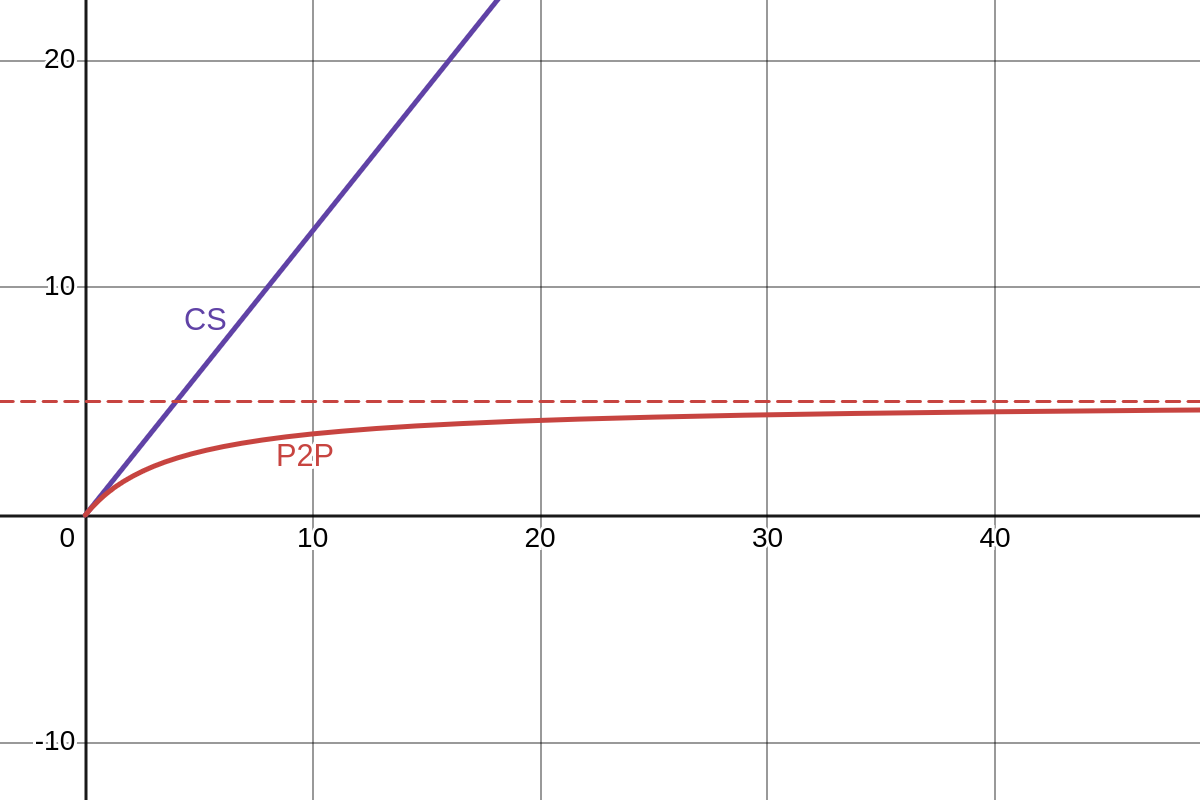
\includegraphics[scale=0.3]{../figures/cs_p2p_ft.png}
\end{center}
\end{minipage}

\subsection{Protocollo BitTorrent}
Approfondiamo le reti P2P, e le \textit{overlay network}, studiando un protocollo reale: il \textbf{protocollo BitTorrent}.

In BitTorrent non è previsto un server centrale che distribuisce il file.
Ogni file è diviso in più \textbf{chunk}, solitamente di 256 KiB ciascuno.

Un \textbf{torrent} è un gruppo di peer che si impegnano a scambiarsi chunk di un file.
Un server più o meno centralizzato detto \textbf{tracker} traccia i peer che partecipano ad un torrent.

\begin{itemize}
	\item 
Quando un utente vuole scaricare un file, chiede al tracker la lista dei peer che partecipano al torrent dedicato a quel file.
Solitamente questo è un \textit{metafile} che contiene l'IP del tracker, a cui si può quindi richiedere il torrent vero e proprio. 

	\item
I peer che l'utente riceve vengono detti \textbf{vicini}: sono connessi da una connessione TCP, e possono quindi scambiarsi dei messaggi (chunk del file).
Possiamo definire così gli utenti collegati ad un torrent:
\begin{itemize}
	\item \textbf{Leecher}: (\textit{"sanguisughe"}), non hanno una copia completa del file e lo stanno ancora scaricando;
	\item \textbf{Seeders}: (\textit{"alimentatori"}), hanno già il file, e lo rendono disponibile agli altri.
\end{itemize}

	\item
Il trasferimento da seeder a leecher si fa un chunk per volta, adottando una politica \textbf{Rarest-First} (\textit{RF}): si inizia a scaricare dal chunk che meno peer sul torrent hanno disponibile. Questo è chiaramente mirato a ottenere i chunk che potrebbero sparire dalla rete il prima possibile.

La lista dei chunk disponibili è fatta richiedendo periodicamente a ogni peer quali chunk possiedono.

	\item 
		Man di mano che i leecher ottengono chunk, devono anche iniziare a rimetterli nella rete ai leecher nuovi arrivati. Su BitTorrent si usa la politica \textbf{Tit for Tat} (\textit{TT}): si inviano chunk ai 4 peer che ci stanno inviando chunk a frequenza più alta.
		Questi top 4 vengono ricalcolati ogni 10 secondi, e gli altri vengono \textit{"strozzati"} (non più serviti).

		Questo significa che i peer potrebbero legarsi eccessivamente fra di loro: ogni 30 secondi si sceglie allora un'altro peer a caso, facendo una previsione \textit{ottimistica} (quel peer potrebbe arrivare fra i nuovi top 4 più frequenti).

		In ogni caso, l'obiettivo è quello di trovare buoni partner per il trasferimento file, in modo da ottenere il file più velocemente possibile.
\end{itemize}

La politica \textit{Tit for Tat} di BitTorrent è chiaramente pensata per scoraggiare i \textit{freeloader}: non si può scaricare se non si dà qualcosa in cambio, cioè si partecipa attivamente al trasferimento rimettendo chunk in circolo.

\subsection{Streaming video e CDN}
Vediamo come si possono creare tecnologie per il trasferimento massiccio di contenuti multimediali, con riferimento allo \textbf{streaming video} e i \textbf{CDN} (\textit{Content Distribution Networks}).

I problemi sono la \textbf{scala} (come raggiungere molti utenti?) e l'\textbf{eterogeneità} (diversi utenti hanno diverse caratteristiche di trasmissione, dispositivi di visualizzazione, ecc...).

La soluzione è infrastruttura \textbf{distribuita} al livello application.

\subsubsection{Video}
Un \textbf{video} è una sequenza di immagini dette \textbf{frame} mostrate a frequenza costante (standard 24, 30, e 60 \textbf{FPS} (\textit{Frames Per Second})).
Un \textbf{frame} è un'array di pixel, dove ogni pixel è rappresentato da 3 valori (corrispondenti ai colori primari additivi \textit{rosso}, \textit{verde} e \textit{blu}).

La tecnica del \textbf{coding} consiste nell'usare ridondanza intrinseca dentro e fra i frame per ridurre i bit usati nel processo di codifica:
\begin{itemize}
	\item Si usa la correlazione \textbf{spaziale}, dentro i singoli frame;
	\item Si usa la correlazione \textbf{temporale}, fra diversi frame.
\end{itemize}

Esistono più tipi di coding, fra cui notiamo:
\begin{itemize}
	\item \textbf{CBR} (\textit{Constant Bit Rate}), a bitrate costante;
	\item \textbf{VBR} (\textit{Variable Bit Rate}), a bitrate variabile;
\end{itemize}

\subsubsection{Streaming}
Lo \textbf{streaming} di video allocati in remoto consiste nel spedire contenuti video abbastanza velocemente da renderli disponibile in \textit{tempo reale} (a differenza del semplice download, che prevede una fase iniziale di acquisizione e una seconda fase di visualizzazione quando il file è ormai già tutto sul disco locale).

Il server dovrà quindi inviare al client frame con una frequenza prefissata (quella del contenuto video), e il client potrà mostrarli appena arrivati.
Assunta una rete ideale, quindi a ritardo \textit{costante}, questo ci permetterebe di visualizzare il video così com'è (al pari di tale ritardo costante).

Purtroppo la rete non è ideale, e il ritardo è quindi \textit{variabile} nel tempo.
Possiamo quindi sfruttare il processo del \textbf{buffering}: aspettiamo un po' lato client prima di mostrare i frame (per un tempo detto \textit{client playout delay}), mettendoli nel frattempo in un \textit{buffer} di memoria.
Quando iniziamo a visualizzare i frame, ci aspettiamo che il buffer sia abbastanza \textit{"pieno"} da permettere la visualizzazione di un segmento di video abbastanza lungo da permettere l'acquisizione dei frame successivi, e così via. 

\end{document}

\documentclass[a4paper,11pt]{article}
\usepackage[a4paper, margin=8em]{geometry}

% usa i pacchetti per la scrittura in italiano
\usepackage[french,italian]{babel}
\usepackage[T1]{fontenc}
\usepackage[utf8]{inputenc}
\frenchspacing 

% usa i pacchetti per la formattazione matematica
\usepackage{amsmath, amssymb, amsthm, amsfonts}

% usa altri pacchetti
\usepackage{gensymb}
\usepackage{hyperref}
\usepackage{standalone}

\usepackage{colortbl}

\usepackage{xstring}
\usepackage{karnaugh-map}

% imposta il titolo
\title{Appunti Reti Informatiche}
\author{Luca Seggiani}
\date{2025}

% imposta lo stile
% usa helvetica
\usepackage[scaled]{helvet}
% usa palatino
\usepackage{palatino}
% usa un font monospazio guardabile
\usepackage{lmodern}

\renewcommand{\rmdefault}{ppl}
\renewcommand{\sfdefault}{phv}
\renewcommand{\ttdefault}{lmtt}

% circuiti
\usepackage{circuitikz}
\usetikzlibrary{babel}

% testo cerchiato
\newcommand*\circled[1]{\tikz[baseline=(char.base)]{
            \node[shape=circle,draw,inner sep=2pt] (char) {#1};}}

% disponi il titolo
\makeatletter
\renewcommand{\maketitle} {
	\begin{center} 
		\begin{minipage}[t]{.8\textwidth}
			\textsf{\huge\bfseries \@title} 
		\end{minipage}%
		\begin{minipage}[t]{.2\textwidth}
			\raggedleft \vspace{-1.65em}
			\textsf{\small \@author} \vfill
			\textsf{\small \@date}
		\end{minipage}
		\par
	\end{center}

	\thispagestyle{empty}
	\pagestyle{fancy}
}
\makeatother

% disponi teoremi
\usepackage{tcolorbox}
\newtcolorbox[auto counter, number within=section]{theorem}[2][]{%
	colback=blue!10, 
	colframe=blue!40!black, 
	sharp corners=northwest,
	fonttitle=\sffamily\bfseries, 
	title=Teorema~\thetcbcounter: #2, 
	#1
}

% disponi definizioni
\newtcolorbox[auto counter, number within=section]{definition}[2][]{%
	colback=red!10,
	colframe=red!40!black,
	sharp corners=northwest,
	fonttitle=\sffamily\bfseries,
	title=Definizione~\thetcbcounter: #2,
	#1
}

% disponi codice
\usepackage{listings}
\usepackage[table]{xcolor}

\definecolor{codegreen}{rgb}{0,0.6,0}
\definecolor{codegray}{rgb}{0.5,0.5,0.5}
\definecolor{codepurple}{rgb}{0.58,0,0.82}
\definecolor{backcolour}{rgb}{0.95,0.95,0.92}

\lstdefinestyle{codestyle}{
		backgroundcolor=\color{black!5}, 
		commentstyle=\color{codegreen},
		keywordstyle=\bfseries\color{magenta},
		numberstyle=\sffamily\tiny\color{black!60},
		stringstyle=\color{green!50!black},
		basicstyle=\ttfamily\footnotesize,
		breakatwhitespace=false,         
		breaklines=true,                 
		captionpos=b,                    
		keepspaces=true,                 
		numbers=left,                    
		numbersep=5pt,                  
		showspaces=false,                
		showstringspaces=false,
		showtabs=false,                  
		tabsize=2
}

\lstdefinestyle{shellstyle}{
		backgroundcolor=\color{black!5}, 
		basicstyle=\ttfamily\footnotesize\color{black}, 
		commentstyle=\color{black}, 
		keywordstyle=\color{black},
		numberstyle=\color{black!5},
		stringstyle=\color{black}, 
		showspaces=false,
		showstringspaces=false, 
		showtabs=false, 
		tabsize=2, 
		numbers=none, 
		breaklines=true
}


\lstdefinelanguage{assembler}{ 
  keywords={AAA, AAD, AAM, AAS, ADC, ADCB, ADCW, ADCL, ADD, ADDB, ADDW, ADDL, AND, ANDB, ANDW, ANDL,
        ARPL, BOUND, BSF, BSFL, BSFW, BSR, BSRL, BSRW, BSWAP, BT, BTC, BTCB, BTCW, BTCL, BTR, 
        BTRB, BTRW, BTRL, BTS, BTSB, BTSW, BTSL, CALL, CBW, CDQ, CLC, CLD, CLI, CLTS, CMC, CMP,
        CMPB, CMPW, CMPL, CMPS, CMPSB, CMPSD, CMPSW, CMPXCHG, CMPXCHGB, CMPXCHGW, CMPXCHGL,
        CMPXCHG8B, CPUID, CWDE, DAA, DAS, DEC, DECB, DECW, DECL, DIV, DIVB, DIVW, DIVL, ENTER,
        HLT, IDIV, IDIVB, IDIVW, IDIVL, IMUL, IMULB, IMULW, IMULL, IN, INB, INW, INL, INC, INCB,
        INCW, INCL, INS, INSB, INSD, INSW, INT, INT3, INTO, INVD, INVLPG, IRET, IRETD, JA, JAE,
        JB, JBE, JC, JCXZ, JE, JECXZ, JG, JGE, JL, JLE, JMP, JNA, JNAE, JNB, JNBE, JNC, JNE, JNG,
        JNGE, JNL, JNLE, JNO, JNP, JNS, JNZ, JO, JP, JPE, JPO, JS, JZ, LAHF, LAR, LCALL, LDS,
        LEA, LEAVE, LES, LFS, LGDT, LGS, LIDT, LMSW, LOCK, LODSB, LODSD, LODSW, LOOP, LOOPE,
        LOOPNE, LSL, LSS, LTR, MOV, MOVB, MOVW, MOVL, MOVSB, MOVSD, MOVSW, MOVSX, MOVSXB,
        MOVSXW, MOVSXL, MOVZX, MOVZXB, MOVZXW, MOVZXL, MUL, MULB, MULW, MULL, NEG, NEGB, NEGW,
        NEGL, NOP, NOT, NOTB, NOTW, NOTL, OR, ORB, ORW, ORL, OUT, OUTB, OUTW, OUTL, OUTSB, OUTSD,
        OUTSW, POP, POPL, POPW, POPB, POPA, POPAD, POPF, POPFD, PUSH, PUSHL, PUSHW, PUSHB, PUSHA, 
				PUSHAD, PUSHF, PUSHFD, RCL, RCLB, RCLW, MOVSL, MOVSB, MOVSW, STOSL, STOSB, STOSW, LODSB, LODSW,
				LODSL, INSB, INSW, INSL, OUTSB, OUTSL, OUTSW
        RCLL, RCR, RCRB, RCRW, RCRL, RDMSR, RDPMC, RDTSC, REP, REPE, REPNE, RET, ROL, ROLB, ROLW,
        ROLL, ROR, RORB, RORW, RORL, SAHF, SAL, SALB, SALW, SALL, SAR, SARB, SARW, SARL, SBB,
        SBBB, SBBW, SBBL, SCASB, SCASD, SCASW, SETA, SETAE, SETB, SETBE, SETC, SETE, SETG, SETGE,
        SETL, SETLE, SETNA, SETNAE, SETNB, SETNBE, SETNC, SETNE, SETNG, SETNGE, SETNL, SETNLE,
        SETNO, SETNP, SETNS, SETNZ, SETO, SETP, SETPE, SETPO, SETS, SETZ, SGDT, SHL, SHLB, SHLW,
        SHLL, SHLD, SHR, SHRB, SHRW, SHRL, SHRD, SIDT, SLDT, SMSW, STC, STD, STI, STOSB, STOSD,
        STOSW, STR, SUB, SUBB, SUBW, SUBL, TEST, TESTB, TESTW, TESTL, VERR, VERW, WAIT, WBINVD,
        XADD, XADDB, XADDW, XADDL, XCHG, XCHGB, XCHGW, XCHGL, XLAT, XLATB, XOR, XORB, XORW, XORL},
  keywordstyle=\color{blue}\bfseries,
  ndkeywordstyle=\color{darkgray}\bfseries,
  identifierstyle=\color{black},
  sensitive=false,
  comment=[l]{\#},
  morecomment=[s]{/*}{*/},
  commentstyle=\color{purple}\ttfamily,
  stringstyle=\color{red}\ttfamily,
  morestring=[b]',
  morestring=[b]"
}

\lstset{language=assembler, style=codestyle}

% disponi sezioni
\usepackage{titlesec}

\titleformat{\section}
	{\sffamily\Large\bfseries} 
	{\thesection}{1em}{} 
\titleformat{\subsection}
	{\sffamily\large\bfseries}   
	{\thesubsection}{1em}{} 
\titleformat{\subsubsection}
	{\sffamily\normalsize\bfseries} 
	{\thesubsubsection}{1em}{}

% tikz
\usepackage{tikz}

% float
\usepackage{float}

% grafici
\usepackage{pgfplots}
\pgfplotsset{width=10cm,compat=1.9}

% disponi alberi
\usepackage{forest}

\forestset{
	rectstyle/.style={
		for tree={rectangle,draw,font=\large\sffamily}
	},
	roundstyle/.style={
		for tree={circle,draw,font=\large}
	}
}

% disponi algoritmi
\usepackage{algorithm}
\usepackage{algorithmic}
\makeatletter
\renewcommand{\ALG@name}{Algoritmo}
\makeatother

% disponi numeri di pagina
\usepackage{fancyhdr}
\fancyhf{} 
\fancyfoot[L]{\sffamily{\thepage}}

\makeatletter
\fancyhead[L]{\raisebox{1ex}[0pt][0pt]{\sffamily{\@title \ \@date}}} 
\fancyhead[R]{\raisebox{1ex}[0pt][0pt]{\sffamily{\@author}}}
\makeatother

\begin{document}
% sezione (data)
\section{Lezione del 10-10-25}

% stili pagina
\thispagestyle{empty}
\pagestyle{fancy}

% testo
Torniamo sull'argomento dello streaming video.

\subsection{Tecniche avanzate per lo streaming}
Avevamo introdotto l'idea del \textbf{playout delay}, dove bufferizzaviamo i dati video in ingresso per "spostare in avanti" in qualche modo la zona di dati compromessa dal \textit{jitter} (irregolarità) della rete.

Visto che il jitter può essere massiccio, e la quantità di dati da inviare non indifferente, esistono alcune strategie più effiaci come ad esempio \textbf{DASH}.

\subsubsection{DASH}
\textbf{DASH} (\textit{Dynamic, Adaptive Streaming over HTTP}) è una tecnologia che prevede di memorizzare i file video in più chunk, ogninuo memorizzato con ridondaza a diversi bitrate. Un \textit{manifest file} fornirà gli URL di tutti i chunk, individuati quindi da indice nel video e livello di compressione.

Il \textit{client} dovrà a questo punto misurare la velocità di trasmissione del server, e quindi consultare il manifest file: sulla base delle misurazioni fatte richiede il chunk di qualità massima sostenibile alla largezza di banda corrente. In questo modo può variare la qualità del video nel tempo, in modo da rispondere in maniera abbastanza elastica alle irregolarità della rete.

Questo richiede \textit{"intelligenza"} dal client: questo deve sapere:
\begin{itemize}
	\item \textit{Quando} richiedere i chunk in modo da non incorrere né in starvation (restare senza chunk) né in overflow (non avere più spazio per i chunk);
	\item \textit{A che bitrate} richiedere i chunk sulla base della banda disponibile;
	\item \textit{Dove} richiedere i chunk: se i server sono duplicati dovrà scegliere il più efficiente.
\end{itemize}

\subsection{CDN}
Vediamo un'altra tecnologia, questa volta riguardante la \textit{scalabilità} dei server che forniscono gigantesche quantità di contenuti video a numeri altrettanto grandi di utenti, simultaneamente, in tutto il mondo.
Questo è il problema che viene affrontato dai \textbf{CDN} (\textit{Content Distribution Network}).

L'idea è di copiare e servire diverse copie dei video su diversi server in siti geograficamente distribuiti.
Esistono due approcci per la dislocazione di tali server:
\begin{itemize}
	\item \textbf{Enter deep}: usare server CDN vicini agli access network: l'idea è di spostarsi il più vicino possibile agli utenti;
	\item \textbf{Bring home}: meno cluster, più grandi, distribuiti in \textbf{POP} (\textit{Points Of Presence}) \textit{vicini} ma non \textit{sulla} rete di accesso degli utenti. 
\end{itemize}

Facciamo un'esempio pratico, guardando al processo che un servizio di distribuzione segue per fornire un contenuto a un utente.
Abbiamo che il meccanismo principale di redirezione è realizzato sfruttando il DNS:
\begin{itemize}
	\item Il CDN (diciamo \lstinline|kingcdn.com|) mantiene più copie del contenuto su diversi \textit{nodi} CDN (magari \lstinline|kingcdn.com/<slug-contenuto-1>|, \lstinline|kingcdn.com/<slug-contenuto-2>|, ecc...). 
	\item Il servizio di distribuzione rende disponibile il contenuto a \lstinline|video.netcinema.com/<slug-contenuto>|;
	\item L'utente richiede un contenuto dal CDN, collegandosi a \lstinline|netcinema.com| e navigando fino al contenuto richiesto a \lstinline|video.netcinema.com/<slug-contenuto>| (l'opzione più probabile è che questo contenuto si trovi in un blocco HTML di tipo \lstinline|<video>|);
	\item A questo punto, il DNS locale dell'utente chiede l'IP di \lstinline|video.netcinema.com| ai server autoritativi di \lstinline|netcinema.com|, che risponde con un record CNAME corrispondente all'IP del server autoritativo di \lstinline|kingcdn.com|;
		\item L'utente viene quindi rediretto verso il nodo più vicino (potrebbe anche scegliere un'altro percorso se si verificassero variazioni (in peggio) del servizio). Da qui in poi il video è trasmesso dal nodo del CDN su HTTP.
\end{itemize}

\subsection{Programmazione socket}
Abbiamo introdotto il concetto di \textbf{socket} (dall'inglese per \textit{presa}) come astrazione della comunicazione in rete per i processi in esecuzione su un S/O.

Lato pratico, il S/O renderà disponibili chiamate a sistema per effettuare almeno alcune operazioni base:
\begin{itemize}
	\item Apertura di un socket: questo potrà essere \textbf{TCP} o \textbf{UDP};
	\item Invio di dati al socket (o scrittura sul socket);
	\item Ricezione di dati al socket (o lettura dal socket).
\end{itemize}

Ricordiamo che il TCP è un protocollo orientato alla connessione, sicuro e affidabile, mentre UDP è un protocollo semplice per il trasferimento diretto ma non affidabile di dati.

\subsection{Reti in connessione diretta}
Finite le applicazioni, riprendiamo il discorso dal \textit{basso}. Se avevamo discusso come creare applicazioni che sfruttassero la rete, adesso vogliamo discutere come la rete riesce in primo luogo a trasmettere bit fra più processi, o anche solo fra più calcolatori.

Iniziamo col considerare come nodi \textbf{adiacenti} nella rete comunicano fra di loro, cioè come 2 host con apposite interfacce di rete comunicano attraverso una connessione diretta: il caso più semplice è quello di un link punto-punto fisico.

Ci sono già diversi problemi da analizzare: come rendere la comunicazione \textbf{affidabile} (\textit{framing}, \textit{rilevamento errori} e \textit{correzione}, ecc...).
Introdurremo quindi il protocollo \textbf{PPP} (\textit{Point to Point Protocol}), i protcolli ad \textbf{accesso multiplo}, e le \textbf{LAN} (\textit{Local Area Network}).

\subsection{Link punto-punto fisici}
Supponiamo di avere 2 host (2 macchine) che vogliono comunicare fra di loro. Questi saranno provvisti ciascuno di un interfaccia per una porta seriale che potranno comandare (alto o basso), e le loro porte seriali saranno collegate da un link di qualche tipo (rame, fibra ottica, ecc...).

Le porte seriali permettono la \textbf{codifica} di bit attraverso variazioni di stato del mezzo fisico del link.

L'interfaccia della macchina mittente è detta \textbf{trasmettitore}, mentre l'interfaccia della macchina destinatario è detta \textbf{ricevitore}: bisognerà stabilire un protocollo per la comunicazione fra questi.

In questo caso il protocollo è semplice il \textit{trasmettitore} dovrà occuparsi di \textbf{codificare} sequenze di bit in variazioni di stato sul mezzo di link, mentre il \textit{ricevitore} dovrà occuparsi di \textbf{decodificare} tali variazioni di stato riportandole in bit sulla macchina destinatario.

\subsubsection{Data link}
Una caratteristica fondamentale dei link è che sono \textit{inaffidabili}: il canale di trasmissione non è mai ideale (degradazione del segnale, rumore, interferenze, ecc....) e quindi la sequenza codificata potrebbe arrivare al ricevitore radicalmente cambiata rispetto a quella iniziale.

Chiameremo \textit{bit error rate} la frequenza di bit persi sul mezzo di comunicazione. 

Per gestire l'inaffidabilità introdurremo un livello superiore a quello di \textbf{link fisico}, detto di \textbf{link dati} (\textit{data link} o anche \textit{livello logico}).
\begin{itemize}
	\item La prima cosa che prevede il data link è il \textbf{framing}: si divide la comunicazione in \textit{payaload} (insiemi di bit), e si incapsulano i tali payload fra \textit{header} e \textit{trailer} (sostanzialmente intestazioni e terminazioni), andando a formare il cosiddetto \textbf{frame}. Da qui in poi, con frame intenderemo sia l'intero frame che il suo payload a seconda del contesto. 
		
		Nell'\textbf{header} potremmo inserire diverse informazioni: prima fra tutte l'indice del frame nell'intero blocco di dati da trasferire.
		
		Se la frequenza di errore è comparabile con la lunghezza dei frame, avremo sicuramente perdite di dati: riducendo la lunghezza dei frame potremmo avere più fortuna.

		Questa tecnica introduce chiaramente un certo \textit{overhead} di trasmissione, dato dal dover introdurre header e trailer. Ci permette però di dividere la trasmissione in unità contenute, su cui è più semplice fare controllo degli errori;
	\item Altri servizi sono forniti per il controllo degli errori di trasmissione: l'\textbf{error detection} mira a rilevare gli errori, mentre l'\textbf{error correction} mira a rilevarli e correggerli. Questo è piuttosto semplice nel caso di trasmissioni binarie: assunto di avere un rilevamento dell'errore granulare al bit, correggerlo significherà semplicemente invertirlo.
		
		Una soluzione alternativa è comunque quella della \textbf{ritrasmissione} dei dati in errore, che implica però una comunicazione all'\textit{indietro}, dal ricevitore al trasmettitore per la segnalazione dei frame corrotti.

	\item Ci sono poi altri servizi che potremmo voler fornire: ad esempio il \textbf{controllo di flusso} che permetta di moderare in qualche modo la frequenza di trasmissione. Ad esempio il ricevitore potrebbe voler segnalare al trasmettitore di dover ridurre il bitrate, magari per problemi di overflow.

	\item Infine, vogliamo distinguere se offriamo servizi \textbf{half-duplex} o \textbf{full-duplex}:
		\begin{itemize}
			\item \textbf{Half-duplex}: entrambi i nodi possono trasmettere, ma solo uno per volta;
			\item \textbf{Full-duplex}: entrambi i nodi possono trasmettere, in \textit{parallelo} (quindi contemporaneamente).
		\end{itemize}

		Configurazioni dove solo un nodo può trasmettere sono dette \textbf{simplex}.
\end{itemize}

\subsubsection{NIC}
Il livello data link è implementato nella cosiddetta \textbf{NIC} (\textit{Network Interface Card}) all'interno di ogni host sulla rete. Questa implementa il livello data link e di conseguenza il livello fisico. Può essere Ethernet, WiFi, ecc...

La NIC è collegata al bus periferiche di un calcolatore (ad esempio bus PCI) e implementa una o più delle funzionalità offerte dal livello data link.
Fa questo combinando \textit{hardware}, \textit{software} e \textit{firmware}: l'importante è che sia capace di offrire al calcolatore i datagrammi inviati al livello data link (in questo sia il NIC che il calcolatore vedono il livello data link).

\end{document}

\documentclass[a4paper,11pt]{article}
\usepackage[a4paper, margin=8em]{geometry}

% usa i pacchetti per la scrittura in italiano
\usepackage[french,italian]{babel}
\usepackage[T1]{fontenc}
\usepackage[utf8]{inputenc}
\frenchspacing 

% usa i pacchetti per la formattazione matematica
\usepackage{amsmath, amssymb, amsthm, amsfonts}

% usa altri pacchetti
\usepackage{gensymb}
\usepackage{hyperref}
\usepackage{standalone}

\usepackage{colortbl}

\usepackage{xstring}
\usepackage{karnaugh-map}

% imposta il titolo
\title{Appunti Reti Informatiche}
\author{Luca Seggiani}
\date{2025}

% imposta lo stile
% usa helvetica
\usepackage[scaled]{helvet}
% usa palatino
\usepackage{palatino}
% usa un font monospazio guardabile
\usepackage{lmodern}

\renewcommand{\rmdefault}{ppl}
\renewcommand{\sfdefault}{phv}
\renewcommand{\ttdefault}{lmtt}

% circuiti
\usepackage{circuitikz}
\usetikzlibrary{babel}

% testo cerchiato
\newcommand*\circled[1]{\tikz[baseline=(char.base)]{
            \node[shape=circle,draw,inner sep=2pt] (char) {#1};}}

% disponi il titolo
\makeatletter
\renewcommand{\maketitle} {
	\begin{center} 
		\begin{minipage}[t]{.8\textwidth}
			\textsf{\huge\bfseries \@title} 
		\end{minipage}%
		\begin{minipage}[t]{.2\textwidth}
			\raggedleft \vspace{-1.65em}
			\textsf{\small \@author} \vfill
			\textsf{\small \@date}
		\end{minipage}
		\par
	\end{center}

	\thispagestyle{empty}
	\pagestyle{fancy}
}
\makeatother

% disponi teoremi
\usepackage{tcolorbox}
\newtcolorbox[auto counter, number within=section]{theorem}[2][]{%
	colback=blue!10, 
	colframe=blue!40!black, 
	sharp corners=northwest,
	fonttitle=\sffamily\bfseries, 
	title=Teorema~\thetcbcounter: #2, 
	#1
}

% disponi definizioni
\newtcolorbox[auto counter, number within=section]{definition}[2][]{%
	colback=red!10,
	colframe=red!40!black,
	sharp corners=northwest,
	fonttitle=\sffamily\bfseries,
	title=Definizione~\thetcbcounter: #2,
	#1
}

% disponi codice
\usepackage{listings}
\usepackage[table]{xcolor}

\definecolor{codegreen}{rgb}{0,0.6,0}
\definecolor{codegray}{rgb}{0.5,0.5,0.5}
\definecolor{codepurple}{rgb}{0.58,0,0.82}
\definecolor{backcolour}{rgb}{0.95,0.95,0.92}

\lstdefinestyle{codestyle}{
		backgroundcolor=\color{black!5}, 
		commentstyle=\color{codegreen},
		keywordstyle=\bfseries\color{magenta},
		numberstyle=\sffamily\tiny\color{black!60},
		stringstyle=\color{green!50!black},
		basicstyle=\ttfamily\footnotesize,
		breakatwhitespace=false,         
		breaklines=true,                 
		captionpos=b,                    
		keepspaces=true,                 
		numbers=left,                    
		numbersep=5pt,                  
		showspaces=false,                
		showstringspaces=false,
		showtabs=false,                  
		tabsize=2
}

\lstdefinestyle{shellstyle}{
		backgroundcolor=\color{black!5}, 
		basicstyle=\ttfamily\footnotesize\color{black}, 
		commentstyle=\color{black}, 
		keywordstyle=\color{black},
		numberstyle=\color{black!5},
		stringstyle=\color{black}, 
		showspaces=false,
		showstringspaces=false, 
		showtabs=false, 
		tabsize=2, 
		numbers=none, 
		breaklines=true
}


\lstdefinelanguage{assembler}{ 
  keywords={AAA, AAD, AAM, AAS, ADC, ADCB, ADCW, ADCL, ADD, ADDB, ADDW, ADDL, AND, ANDB, ANDW, ANDL,
        ARPL, BOUND, BSF, BSFL, BSFW, BSR, BSRL, BSRW, BSWAP, BT, BTC, BTCB, BTCW, BTCL, BTR, 
        BTRB, BTRW, BTRL, BTS, BTSB, BTSW, BTSL, CALL, CBW, CDQ, CLC, CLD, CLI, CLTS, CMC, CMP,
        CMPB, CMPW, CMPL, CMPS, CMPSB, CMPSD, CMPSW, CMPXCHG, CMPXCHGB, CMPXCHGW, CMPXCHGL,
        CMPXCHG8B, CPUID, CWDE, DAA, DAS, DEC, DECB, DECW, DECL, DIV, DIVB, DIVW, DIVL, ENTER,
        HLT, IDIV, IDIVB, IDIVW, IDIVL, IMUL, IMULB, IMULW, IMULL, IN, INB, INW, INL, INC, INCB,
        INCW, INCL, INS, INSB, INSD, INSW, INT, INT3, INTO, INVD, INVLPG, IRET, IRETD, JA, JAE,
        JB, JBE, JC, JCXZ, JE, JECXZ, JG, JGE, JL, JLE, JMP, JNA, JNAE, JNB, JNBE, JNC, JNE, JNG,
        JNGE, JNL, JNLE, JNO, JNP, JNS, JNZ, JO, JP, JPE, JPO, JS, JZ, LAHF, LAR, LCALL, LDS,
        LEA, LEAVE, LES, LFS, LGDT, LGS, LIDT, LMSW, LOCK, LODSB, LODSD, LODSW, LOOP, LOOPE,
        LOOPNE, LSL, LSS, LTR, MOV, MOVB, MOVW, MOVL, MOVSB, MOVSD, MOVSW, MOVSX, MOVSXB,
        MOVSXW, MOVSXL, MOVZX, MOVZXB, MOVZXW, MOVZXL, MUL, MULB, MULW, MULL, NEG, NEGB, NEGW,
        NEGL, NOP, NOT, NOTB, NOTW, NOTL, OR, ORB, ORW, ORL, OUT, OUTB, OUTW, OUTL, OUTSB, OUTSD,
        OUTSW, POP, POPL, POPW, POPB, POPA, POPAD, POPF, POPFD, PUSH, PUSHL, PUSHW, PUSHB, PUSHA, 
				PUSHAD, PUSHF, PUSHFD, RCL, RCLB, RCLW, MOVSL, MOVSB, MOVSW, STOSL, STOSB, STOSW, LODSB, LODSW,
				LODSL, INSB, INSW, INSL, OUTSB, OUTSL, OUTSW
        RCLL, RCR, RCRB, RCRW, RCRL, RDMSR, RDPMC, RDTSC, REP, REPE, REPNE, RET, ROL, ROLB, ROLW,
        ROLL, ROR, RORB, RORW, RORL, SAHF, SAL, SALB, SALW, SALL, SAR, SARB, SARW, SARL, SBB,
        SBBB, SBBW, SBBL, SCASB, SCASD, SCASW, SETA, SETAE, SETB, SETBE, SETC, SETE, SETG, SETGE,
        SETL, SETLE, SETNA, SETNAE, SETNB, SETNBE, SETNC, SETNE, SETNG, SETNGE, SETNL, SETNLE,
        SETNO, SETNP, SETNS, SETNZ, SETO, SETP, SETPE, SETPO, SETS, SETZ, SGDT, SHL, SHLB, SHLW,
        SHLL, SHLD, SHR, SHRB, SHRW, SHRL, SHRD, SIDT, SLDT, SMSW, STC, STD, STI, STOSB, STOSD,
        STOSW, STR, SUB, SUBB, SUBW, SUBL, TEST, TESTB, TESTW, TESTL, VERR, VERW, WAIT, WBINVD,
        XADD, XADDB, XADDW, XADDL, XCHG, XCHGB, XCHGW, XCHGL, XLAT, XLATB, XOR, XORB, XORW, XORL},
  keywordstyle=\color{blue}\bfseries,
  ndkeywordstyle=\color{darkgray}\bfseries,
  identifierstyle=\color{black},
  sensitive=false,
  comment=[l]{\#},
  morecomment=[s]{/*}{*/},
  commentstyle=\color{purple}\ttfamily,
  stringstyle=\color{red}\ttfamily,
  morestring=[b]',
  morestring=[b]"
}

\lstset{language=assembler, style=codestyle}

% disponi sezioni
\usepackage{titlesec}

\titleformat{\section}
	{\sffamily\Large\bfseries} 
	{\thesection}{1em}{} 
\titleformat{\subsection}
	{\sffamily\large\bfseries}   
	{\thesubsection}{1em}{} 
\titleformat{\subsubsection}
	{\sffamily\normalsize\bfseries} 
	{\thesubsubsection}{1em}{}

% tikz
\usepackage{tikz}

% float
\usepackage{float}

% grafici
\usepackage{pgfplots}
\pgfplotsset{width=10cm,compat=1.9}

% disponi alberi
\usepackage{forest}

\forestset{
	rectstyle/.style={
		for tree={rectangle,draw,font=\large\sffamily}
	},
	roundstyle/.style={
		for tree={circle,draw,font=\large}
	}
}

% disponi algoritmi
\usepackage{algorithm}
\usepackage{algorithmic}
\makeatletter
\renewcommand{\ALG@name}{Algoritmo}
\makeatother

% disponi numeri di pagina
\usepackage{fancyhdr}
\fancyhf{} 
\fancyfoot[L]{\sffamily{\thepage}}

\makeatletter
\fancyhead[L]{\raisebox{1ex}[0pt][0pt]{\sffamily{\@title \ \@date}}} 
\fancyhead[R]{\raisebox{1ex}[0pt][0pt]{\sffamily{\@author}}}
\makeatother

\begin{document}
% sezione (data)
\section{Lezione del 13-10-25}

% stili pagina
\thispagestyle{empty}
\pagestyle{fancy}

% testo
\subsection{Rilevamento errori}
Il \textit{rilevamento degli errori} (\textbf{error detection}) è il meccanismo attraverso il cui verifichiamo se i dati arrivati attraverso il link fisico sono corretti.

Dobbiamo innanzitutto stabilire un codice di \textbf{rilevamento} degli errori.
Per ogni frame di livello Datalink trasmettiamo $d$ bit di dati (i bit $D$) e $r$ bit di \textit{rilevamento errore}, o di \textbf{ridondanza} (i bit $R$). Minuscolo è il numero di bit, maiuscolo è il campo di bit vero e proprio.
Sia i bit $D$ che i bit $R$ vengono trasmessi attraverso il link, che ricordiamo è \textit{suscettibile ad errori}.

Per ricavare i bit $R$ si applica una certa funzione $H()$ (sostanzialmente di \textit{hashing}) sui bit $D$. Assunto che mittente e destinatario usino la stessa funzione $H()$, una volta ricevuti i dati il destinatario potrà applicare $H()$ sui bit $D$ ricevuti e ottenere la sua copia dei bit $R$ da confrontare con quelli ricevuti.

Se i bit $R$ corrispondono non ci sono stati errori (a meno della sfortunata circostanza in cui sia i bit $D$ che $R$ sono stati alterati per risultare erroneamente corretti, si sceglie la funzione $H()$ in modo che questo sia difficilmente vero), altrimenti qualcosa è andato storto nella trasmissione sul link.

I bit $R$, nel contesto del \textit{framing} visto in 9.5.1, vengono inseriti nel \textit{trailer} del frame.

\subsubsection{Algoritmi di rilevamento errori}
Vediamo alcune possibili funzioni $H()$ usate per fare rilevamento errori.

\begin{itemize}
	\item \textbf{Parity checking}: posto che si voglia trasferire una parola da $d$ bit: si sceglie un solo bit $R$ di ridondanza, determinato come segue:
		\begin{itemize}
			\item Se il numero di bit a 1 fra i bit $D$ è pari, si imposta il bit in $R$ a 1;
			\item Se il numero di bit a 1 fra i bit $D$ è dispari, si imposta il bit in $R$ a 0.
		\end{itemize}
		In questo caso il bit in $R$ viene detto \textbf{bit di parità} (\textit{parity bit}). Questo algoritmo viene detto di tipo \textbf{even parity}: l'algoritmo opposto si direbbe \textbf{odd parity}.

		Questo algoritmo funziona bene solo nella circostanza in cui il numero di errori sui bit $d$ è dispari (per quanto ci riguarda, 1). Quando si trasferiscono quantità relativamente basse di bit per parola su canali abbastanza affidabili (8, 16, 24 bit su rame o simili) abbiamo che è abbastanza sicuro. Con parole più grandi chiaramente può essere molto più soggetto ad errori.

	\item \textbf{Checksum}: questo sistema, detto della \textit{"somma di controllo"} viene usato in UDP e TCP. Non si riferisce principalmente a frame, quindi parleremo di blocchi di dati generici.

		In questo caso si prende ogni blocco di dati e si divide in frammenti da $n$ bit. Sommando questi frammenti si ottiene un campo $R$ su $r= n$ bit (quindi modulo $2^n$) detto \textit{checksum}, che può essere ricalcolato lato destinatario per fare rilevamento degli errori.

		Questo metodo è più sensibile rispetto al bit di parità, e viene usato perlopiù a livello di \textit{trasporto} UDP o TCP (più che a livello \textit{data link}, dove si fanno altri tipi di controlli meno sensibili).

	\item \textbf{CRC} (\textit{Cyclic Redundancy Check}): questo è il metodo usato più spesso in ambito di \textit{Datalink}.

		Supponiamo di avere $R$ bit dati, e un \textit{pattern} detto \textbf{generatore} $G$ di $r + 1$ bit (dove ricordiamo che $R$ sono i bit di ridondanza e $r$ il loro numero). Mittente e destinatario dovranno entrambi conoscere il generatore.

		L'idea è quindi che in fase di trasmissione si prende un numero $R$ di $r$ bit tale che la concatenazione $D|R$ dei bit $D$ ed $R$ sia divisibile per $G$.
		Notiamo che le somme in CRC si fanno \textit{modulo 2}, quindi senza riporti.
		In questo caso la relazione appena descritta sarà:
		$$
		D \cdot 2^r \oplus R = nG
		$$
		dove $D \cdot 2^r$ è semplicemente lo shift a sinistra di $r$ bit di $D$, $\oplus$ lo XOR (che implementa la somma modulo 2), e $n$ una costante moltiplicativa naturale qualsiasi, che assicura che il lasto sinistro è divisibile per $G$.

		Quando il destinatarrio riceve il frame la verifica è molto semplice: ha $D$ ed $R$ ottenuti sul link fisico, e noto $G$ può effettuare la divisione. Se il resto è diverso da 0, allora si rileva un errore di trasmissione.

		Resta quindi da vedere come $R$ viene calcolato nella pratica.
		Vogliamo:
		$$
		D \times 2^r \oplus R = n G \implies D \times 2^r = n G \oplus R
		$$
		come ci è concesso dalle proprietà dello XOR, per cui $R$ dovrà soddisfare:
		$$
		R = \text{mod}\left( D \times 2^r, G \right)
		$$
		dove \textit{mod} indica il resto della divisione fra i due argomenti (cioè l'operatore modulo).
\end{itemize}

\subsection{Correzione errori}
Dopo aver discusso il \textit{rilevamento degli errori}, vediamo come procedere nella \textbf{correzione degli errori} in caso se ne rilevino.

La soluzione più semplice sarebbe quella di ritrasmettere i frame sbagliati.
Se poi si avesse un algoritmo di rilevamento errori che restituisse esattamente \textit{quali} bit sono errati, basterebbe commutarli per risolvere gli errori.

In questo caso non serve più un codice a \textit{rilevamento} degli errori, ma un codice a \textbf{correzione} degli errori.
Per ogni frame  trasmettiamo $d$ bit di dati (i bit $D$) e $r$ bit di \textit{correzione errore}, o ancora di \textbf{ridondanza} (i bit $EDC$, da \textit{Error Detection Code}).

Questi sono simmetrici al codice definito per il rilevamento errori: la differenza è che dati $D$ ed $EDC$, lato destinatario possiamo rilevare esattamente l'errore di trasmissione (se c'è stato).

\subsubsection{Algoritmi di correzione errori}
Vediamo alcuni (1) modi per calcolare i bit $EDC$ ed effettuare quindi la correzione degli errori.
\begin{itemize}
	\item \textbf{Parity checking bidimensionale}: si sistemano i bit $D$ in una struttura matriciale, e si calcolano i bit di parità per ogni riga e per ogni colonna. 

		Ad esempio, si può dire:
$$
D = \{ 0, 1, 0, ... \} = \{ d_1, d_2, d_3, ... d_d \} \Rightarrow D_m = 
\begin{pmatrix}
	d_{1,1} & d_{1,2} & ... & d_{1,j} \\ 
	d_{2,1} & d_{2,2} & ... & d_{2,j} \\ 
	... & ... & ... & ... \\
	d_{i,1} & d_{i,2} & ... & d_{i,j} \\ 
\end{pmatrix}
$$
Posti $i$ e $j$ tali che $i \cdot j = d$ (numero di bit in $D$).
A questo punto si orla $D_m$ con i bit di parità di \textit{riga} ($\text{parity}_{row}$) e i bit di parità di \textit{colonna} ($\text{parity}_{row}$):
$$
\begin{pmatrix}
	D_m & \text{parity}_{row} \\
	\text{parity}_{col}
\end{pmatrix}
=
\begin{pmatrix}
\begin{array}{cccc|c}
	d_{1,1} & d_{1,2} & ... & d_{1,j} & d_{1, j + 1} \\ 
	d_{2,1} & d_{2,2} & ... & d_{2,j} & d_{2, j + 1} \\ 
	... & ... & ... & ... & ...\\
	d_{i,1} & d_{i,2} & ... & d_{i,j} & d_{i, j + 1} \\ \hline 
	d_{i + 1, 1} & d_{i + 1, 2} & ... & d_{i + 1, j}  \\ 
\end{array}
\end{pmatrix}
$$
dove
$$
\text{parity}_{row}: \quad d_{r, j + 1} = \text{parity}\left( \sum_{c = 1}^{j} d_{r, c} \right)
$$
$$
\text{parity}_{col}: \quad d_{j + 1, c} = \text{parity}\left( \sum_{r = 1}^{i} d_{r, c} \right)
$$

A questo punto un errore su un singolo $d_{r, c}$ verrà rilevato in quanto incrocierà una riga e una colonna (l'intersezione andrà commutata).
Due o più errori su righe e colonne disgiunte veranno similmente rilevati, a meno di casi di errori multipli su più righe e colonnne (che potrebbero addirittura dare falsi positivi).
Infine, un numero pari di errori sulla stessa riga o sulla stessa colonna ci permettono di rilevare, ma non correggere errori (vedremo 2 colonne sbagliate e una riga giusta, o viceversa, senza poter quindi incrociare).

Chiaramente i bit $EDC$ nel trailer saranno molti di più: per la precisione $i + j$.

\end{itemize}

\subsection{Trasferimento dati}
Abbiamo visto alcuni algoritmi di \textit{rilevamento errori}, introdotto l'ipotesi di effettuare un \textit{reinvio} dei dati corrotti nel caso di errori, e visto anche un algoritmo di \textit{rilevamento e correzione errori}.

Vediamo adesso come realizzare un livello superiore a quello data link, riportando indietro l'ipotesi del reinvio dati, cioè il cosiddetto livello \textit{transfer} o \textbf{trasferimento}, che considereremo un livello \textit{affidabile}.

Le considerazioni che facciamo adesso saranno quelle che nel modello OSI vengono implementate nel cosiddetto livello \textbf{transport}.

L'idea è quella di usare i servizi offerti dal livello data link per realizzare un'ulteriore astrazione, quella appunto di \textit{trasferimento affidabile}.

Quello che farà la componentistica di livello transport sarà interagire con un \textit{livello superiore} che fornirà \textit{dati}: questi verranno incapsulati in un \textbf{pacchetto}, a sua volta incluso come \textit{payload} di un frame di livello Datalink, e quindi spedito sulla lniea inaffidabile vista finora.

\subsubsection{Primitive di trasferimento}
Per implementare questo tipo di livello \textit{transfer} ci doteremo quindi di alcune primitive a servizio di un'altro \textit{livello superiore}:
\begin{itemize}
	\item \lstinline|rdt_send()|: chiamata dal livello superiore (nella macchina \textit{trasmettitore}), implementa l'invio sul canale affidabile (cioè implementa un protocollo \textbf{RDT} (\textit{Reliable Data Transfer}));
	\item \lstinline|udt_send()|: implementa l'invio sul canale inaffidabile fino al ricevitore;
	\item \lstinline|rdt_rcv()|: implementa il ricevimento sul canale affidabile lato ricevitore, cioè ottiene i dati sul canale inaffidabile, e li corregge (se necessario); 
	\item \lstinline|deliver_data()|: si occupa di inoltrare i dati ottenuti attraverso il protocollo RDT al livello superiore (nella macchina \textit{ricevitore}).
\end{itemize}

Notiamo che le primitive \lstinline|udt_send()| e \lstinline|rdt_recv()| dovranno implementare un qualche tipo di comunicazione bidirezionale (ad esempio se la \lstinline|rdt_rcv()| vuole chiedere il reinvio di un frame perso).

\subsubsection{Macchine a stati finiti}
Per descrivere il protocollo \textbf{RDT} useremo il formalismo della \textit{macchina a stati finiti} (\textbf{FSM}, \textit{Finite State Machine}).

Una macchina a stati finiti rappresenta un \textit{automa} dotato di \textbf{stati} e \textbf{transizioni} fra tali stati: dato uno stato ed un evento si può determinare la transizione successiva, e quindi come si evolve il protocollo. 

\par\smallskip

Nelle prossime sezioni definiremo \textit{iterativamente} versioni sempre più accurate di RDT rispetto a un qualche protocollo reale.

\subsection{RDT 1.0}
Iniziamo ad iterare sul nostro protocollo \textit{RDT}.
Assumiamo come prime ipotesi, largamente semplificate:
\begin{itemize}
	\item Non ci sono errori di bit;
	\item Non ci sono perdite di frame.
\end{itemize}

Prevederemo quindi FSM diverse per \textit{trasmettitore} e \textit{ricevitore}:
\begin{itemize}
	\item Il trasmettitore invia dati su un canale sottostante;
	\item Il ricevitore legge i dat dal canale sottostante.
\end{itemize}

L'FSM in questo caso sarà semplice:
\begin{center}
	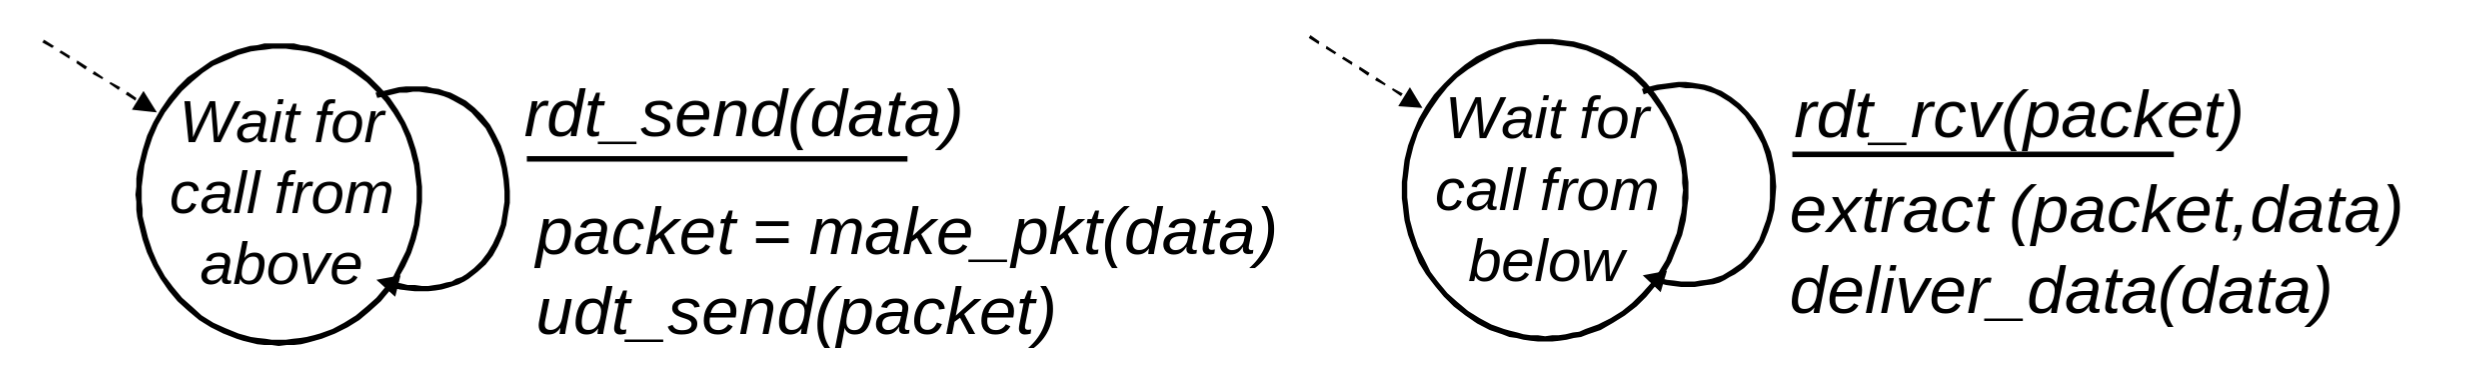
\includegraphics[scale=0.16]{../figures/rdt1fsm.png}
\end{center}
\begin{itemize}
	\item Il trasmettitore avrà il compito di aspettare la chiamata dall'alto, e una volta arrivata di creare un \textit{pacchetto} da spedire sulla linea inaffidabile (incapsulandolo in un opportuno frame);
	\item Il ricevitore avrà il compito di aspettare la chiamata dal basso, e una volta ricevuta ricevere il pacchetto spedito dal trasmettitore. Una volta arrivato, dovrà estrarre i dati dal pacchetto e consegnarli al livello superiore.
\end{itemize}

\subsection{RDT 2.0}
Introduciamo un mezzo di trasmissione inaffidabile che potrebbe avere errori di bit, e presumiamo che tale mezzo implementi un qualche livello sottostante (di tipo data link) che implementa correzione degli errori attraverso CRC o checksum (come visto in 10.1 e 10.2).

Il problema sarà: come riprendersi dagli errori? Abbiamo due modi principali:
\begin{itemize}
	\item \textit{Acknowledgment} (\textbf{ACK}), significa che il ricevitore ha \textit{"capito"}, cioè ha ricevuto il frame correttamente;
	\item \textit{Negative acknowledgment} (\textbf{NAK}), significa che il ricevitor \textit{non ha capito}, cioè non ha ricevuto il frame correttamente.
\end{itemize}

Quando il trasmettitore riceve un \textbf{ACK}, sa di poter procedere con il frame successivo, mentre quando riceve un \textbf{NAK} sa che deve reinviare il frame corrente.

In questo caso l'FSM del trasmettitore ha il seguente aspetto:
\begin{center}
	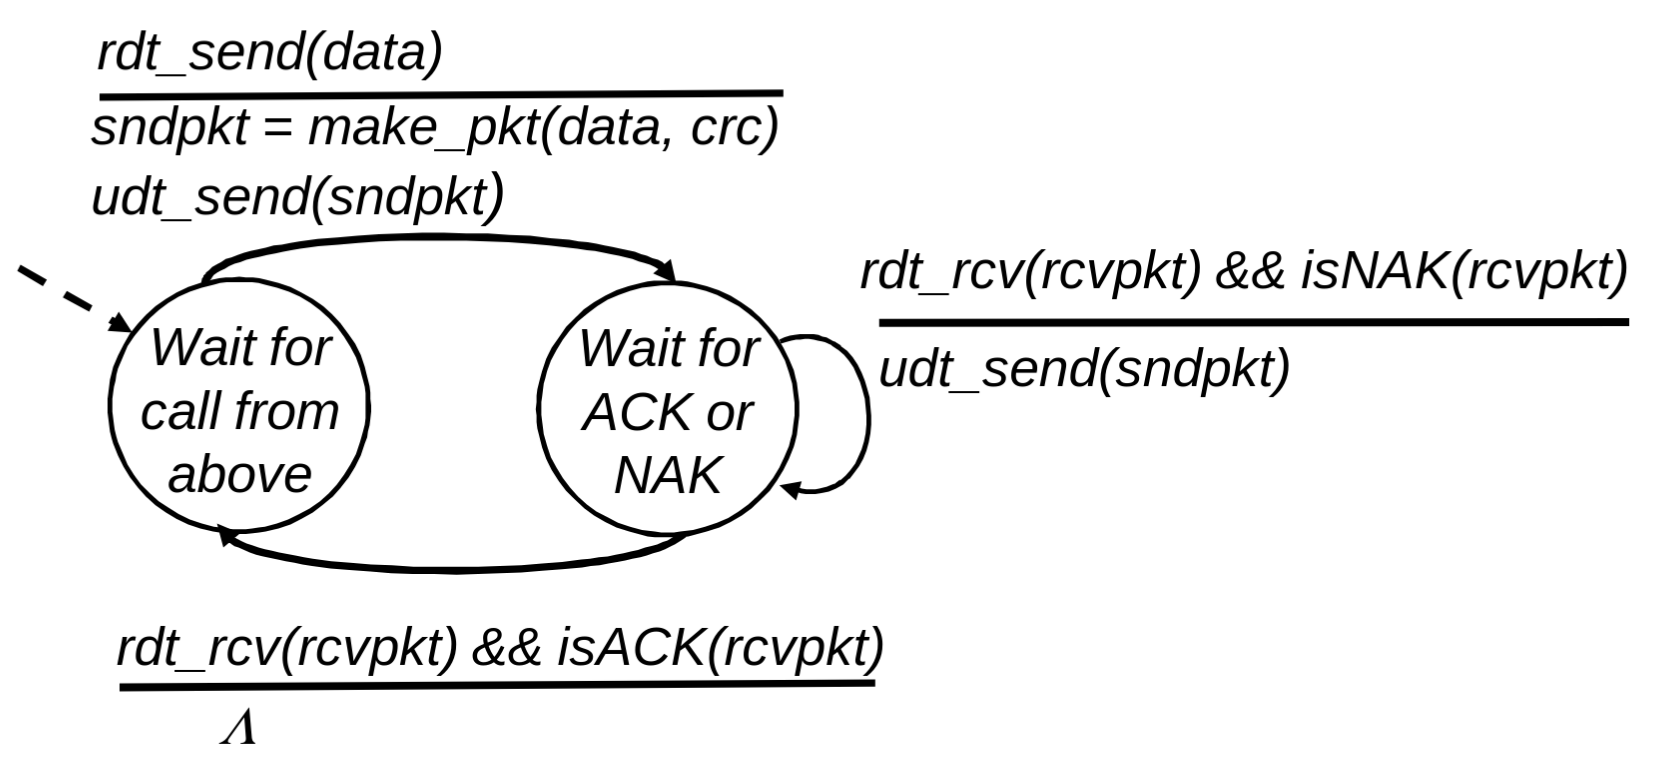
\includegraphics[scale=0.18]{../figures/rdt2fsm.png}
\end{center}
\begin{itemize}
	\item Il trasmettitore avrà il compito, come prima, di aspettare la chiamata dall'alto e quindi inviare il pacchetto sulla linea inaffidabile;
	\item A questo punto dovrà aspettare per un ACK o un NAK dal ricevitore:
		\begin{itemize}
			\item Se riceve un NAK, deve reinviare lo stesso frame;
			\item Altrimenti, cioè se riceve un ACK, deve tornare ad aspettare la chiamata dall'alto per il pacchetto successivo. 
		\end{itemize}
\end{itemize}

Lato ricevitore l'FSM sarà invece:
\begin{center}
	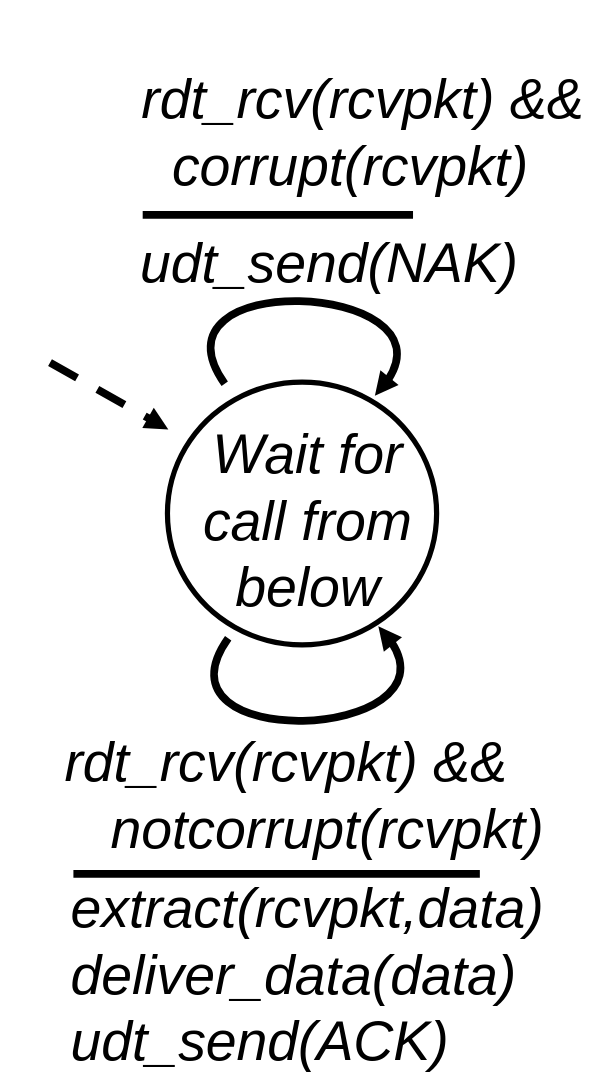
\includegraphics[scale=0.18]{../figures/rdt2fsm2.png}
\end{center}
\begin{itemize}
	\item Il ricevitore dovrà restare in attesa della chiamata dal basso, e rispondere quindi ai pacchetti ricevuti su linea inaffidabile dal trasmettitore;
	\item Valutata la correzione degli errori sul pacchetto ricevuto, dovrà:
		\begin{itemize}
			\item Inviare il NAK nel caso il pacchetto sia corrotto;
			\item Inviare l'ACK e inoltrare il pacchetto al livello superiore nel caso il pacchetto sia stato ricevuto correttamente.
		\end{itemize}
\end{itemize}


\end{document}

\documentclass[a4paper,11pt]{article}
\usepackage[a4paper, margin=8em]{geometry}

% usa i pacchetti per la scrittura in italiano
\usepackage[french,italian]{babel}
\usepackage[T1]{fontenc}
\usepackage[utf8]{inputenc}
\frenchspacing 

% usa i pacchetti per la formattazione matematica
\usepackage{amsmath, amssymb, amsthm, amsfonts}

% usa altri pacchetti
\usepackage{gensymb}
\usepackage{hyperref}
\usepackage{standalone}

\usepackage{colortbl}

\usepackage{xstring}
\usepackage{karnaugh-map}

% imposta il titolo
\title{Appunti Reti Informatiche}
\author{Luca Seggiani}
\date{2025}

% imposta lo stile
% usa helvetica
\usepackage[scaled]{helvet}
% usa palatino
\usepackage{palatino}
% usa un font monospazio guardabile
\usepackage{lmodern}

\renewcommand{\rmdefault}{ppl}
\renewcommand{\sfdefault}{phv}
\renewcommand{\ttdefault}{lmtt}

% circuiti
\usepackage{circuitikz}
\usetikzlibrary{babel}

% testo cerchiato
\newcommand*\circled[1]{\tikz[baseline=(char.base)]{
            \node[shape=circle,draw,inner sep=2pt] (char) {#1};}}

% disponi il titolo
\makeatletter
\renewcommand{\maketitle} {
	\begin{center} 
		\begin{minipage}[t]{.8\textwidth}
			\textsf{\huge\bfseries \@title} 
		\end{minipage}%
		\begin{minipage}[t]{.2\textwidth}
			\raggedleft \vspace{-1.65em}
			\textsf{\small \@author} \vfill
			\textsf{\small \@date}
		\end{minipage}
		\par
	\end{center}

	\thispagestyle{empty}
	\pagestyle{fancy}
}
\makeatother

% disponi teoremi
\usepackage{tcolorbox}
\newtcolorbox[auto counter, number within=section]{theorem}[2][]{%
	colback=blue!10, 
	colframe=blue!40!black, 
	sharp corners=northwest,
	fonttitle=\sffamily\bfseries, 
	title=Teorema~\thetcbcounter: #2, 
	#1
}

% disponi definizioni
\newtcolorbox[auto counter, number within=section]{definition}[2][]{%
	colback=red!10,
	colframe=red!40!black,
	sharp corners=northwest,
	fonttitle=\sffamily\bfseries,
	title=Definizione~\thetcbcounter: #2,
	#1
}

% disponi codice
\usepackage{listings}
\usepackage[table]{xcolor}

\definecolor{codegreen}{rgb}{0,0.6,0}
\definecolor{codegray}{rgb}{0.5,0.5,0.5}
\definecolor{codepurple}{rgb}{0.58,0,0.82}
\definecolor{backcolour}{rgb}{0.95,0.95,0.92}

\lstdefinestyle{codestyle}{
		backgroundcolor=\color{black!5}, 
		commentstyle=\color{codegreen},
		keywordstyle=\bfseries\color{magenta},
		numberstyle=\sffamily\tiny\color{black!60},
		stringstyle=\color{green!50!black},
		basicstyle=\ttfamily\footnotesize,
		breakatwhitespace=false,         
		breaklines=true,                 
		captionpos=b,                    
		keepspaces=true,                 
		numbers=left,                    
		numbersep=5pt,                  
		showspaces=false,                
		showstringspaces=false,
		showtabs=false,                  
		tabsize=2
}

\lstdefinestyle{shellstyle}{
		backgroundcolor=\color{black!5}, 
		basicstyle=\ttfamily\footnotesize\color{black}, 
		commentstyle=\color{black}, 
		keywordstyle=\color{black},
		numberstyle=\color{black!5},
		stringstyle=\color{black}, 
		showspaces=false,
		showstringspaces=false, 
		showtabs=false, 
		tabsize=2, 
		numbers=none, 
		breaklines=true
}


\lstdefinelanguage{assembler}{ 
  keywords={AAA, AAD, AAM, AAS, ADC, ADCB, ADCW, ADCL, ADD, ADDB, ADDW, ADDL, AND, ANDB, ANDW, ANDL,
        ARPL, BOUND, BSF, BSFL, BSFW, BSR, BSRL, BSRW, BSWAP, BT, BTC, BTCB, BTCW, BTCL, BTR, 
        BTRB, BTRW, BTRL, BTS, BTSB, BTSW, BTSL, CALL, CBW, CDQ, CLC, CLD, CLI, CLTS, CMC, CMP,
        CMPB, CMPW, CMPL, CMPS, CMPSB, CMPSD, CMPSW, CMPXCHG, CMPXCHGB, CMPXCHGW, CMPXCHGL,
        CMPXCHG8B, CPUID, CWDE, DAA, DAS, DEC, DECB, DECW, DECL, DIV, DIVB, DIVW, DIVL, ENTER,
        HLT, IDIV, IDIVB, IDIVW, IDIVL, IMUL, IMULB, IMULW, IMULL, IN, INB, INW, INL, INC, INCB,
        INCW, INCL, INS, INSB, INSD, INSW, INT, INT3, INTO, INVD, INVLPG, IRET, IRETD, JA, JAE,
        JB, JBE, JC, JCXZ, JE, JECXZ, JG, JGE, JL, JLE, JMP, JNA, JNAE, JNB, JNBE, JNC, JNE, JNG,
        JNGE, JNL, JNLE, JNO, JNP, JNS, JNZ, JO, JP, JPE, JPO, JS, JZ, LAHF, LAR, LCALL, LDS,
        LEA, LEAVE, LES, LFS, LGDT, LGS, LIDT, LMSW, LOCK, LODSB, LODSD, LODSW, LOOP, LOOPE,
        LOOPNE, LSL, LSS, LTR, MOV, MOVB, MOVW, MOVL, MOVSB, MOVSD, MOVSW, MOVSX, MOVSXB,
        MOVSXW, MOVSXL, MOVZX, MOVZXB, MOVZXW, MOVZXL, MUL, MULB, MULW, MULL, NEG, NEGB, NEGW,
        NEGL, NOP, NOT, NOTB, NOTW, NOTL, OR, ORB, ORW, ORL, OUT, OUTB, OUTW, OUTL, OUTSB, OUTSD,
        OUTSW, POP, POPL, POPW, POPB, POPA, POPAD, POPF, POPFD, PUSH, PUSHL, PUSHW, PUSHB, PUSHA, 
				PUSHAD, PUSHF, PUSHFD, RCL, RCLB, RCLW, MOVSL, MOVSB, MOVSW, STOSL, STOSB, STOSW, LODSB, LODSW,
				LODSL, INSB, INSW, INSL, OUTSB, OUTSL, OUTSW
        RCLL, RCR, RCRB, RCRW, RCRL, RDMSR, RDPMC, RDTSC, REP, REPE, REPNE, RET, ROL, ROLB, ROLW,
        ROLL, ROR, RORB, RORW, RORL, SAHF, SAL, SALB, SALW, SALL, SAR, SARB, SARW, SARL, SBB,
        SBBB, SBBW, SBBL, SCASB, SCASD, SCASW, SETA, SETAE, SETB, SETBE, SETC, SETE, SETG, SETGE,
        SETL, SETLE, SETNA, SETNAE, SETNB, SETNBE, SETNC, SETNE, SETNG, SETNGE, SETNL, SETNLE,
        SETNO, SETNP, SETNS, SETNZ, SETO, SETP, SETPE, SETPO, SETS, SETZ, SGDT, SHL, SHLB, SHLW,
        SHLL, SHLD, SHR, SHRB, SHRW, SHRL, SHRD, SIDT, SLDT, SMSW, STC, STD, STI, STOSB, STOSD,
        STOSW, STR, SUB, SUBB, SUBW, SUBL, TEST, TESTB, TESTW, TESTL, VERR, VERW, WAIT, WBINVD,
        XADD, XADDB, XADDW, XADDL, XCHG, XCHGB, XCHGW, XCHGL, XLAT, XLATB, XOR, XORB, XORW, XORL},
  keywordstyle=\color{blue}\bfseries,
  ndkeywordstyle=\color{darkgray}\bfseries,
  identifierstyle=\color{black},
  sensitive=false,
  comment=[l]{\#},
  morecomment=[s]{/*}{*/},
  commentstyle=\color{purple}\ttfamily,
  stringstyle=\color{red}\ttfamily,
  morestring=[b]',
  morestring=[b]"
}

\lstset{language=assembler, style=codestyle}

% disponi sezioni
\usepackage{titlesec}

\titleformat{\section}
	{\sffamily\Large\bfseries} 
	{\thesection}{1em}{} 
\titleformat{\subsection}
	{\sffamily\large\bfseries}   
	{\thesubsection}{1em}{} 
\titleformat{\subsubsection}
	{\sffamily\normalsize\bfseries} 
	{\thesubsubsection}{1em}{}

% tikz
\usepackage{tikz}

% float
\usepackage{float}

% grafici
\usepackage{pgfplots}
\pgfplotsset{width=10cm,compat=1.9}

% disponi alberi
\usepackage{forest}

\forestset{
	rectstyle/.style={
		for tree={rectangle,draw,font=\large\sffamily}
	},
	roundstyle/.style={
		for tree={circle,draw,font=\large}
	}
}

% disponi algoritmi
\usepackage{algorithm}
\usepackage{algorithmic}
\makeatletter
\renewcommand{\ALG@name}{Algoritmo}
\makeatother

% disponi numeri di pagina
\usepackage{fancyhdr}
\fancyhf{} 
\fancyfoot[L]{\sffamily{\thepage}}

\makeatletter
\fancyhead[L]{\raisebox{1ex}[0pt][0pt]{\sffamily{\@title \ \@date}}} 
\fancyhead[R]{\raisebox{1ex}[0pt][0pt]{\sffamily{\@author}}}
\makeatother

\begin{document}
% sezione (data)
\section{Lezione del 15-10-25}

% stili pagina
\thispagestyle{empty}
\pagestyle{fancy}

% testo
\subsubsection{RDT 2.1}
Avevamo introdotto il protocollo di trasferimento fittizio RDT 2.0.
Questo era basato su segnali ACK/NAK mandati sul livello datalink dal destinatario al mittente.

Un problema che non avevamo considerato è che questi segnali possono venire corrotti, proprio come i dati veri e propri che volevamo trasmettere.
Se il mittente riceve un ACK/NAK corrotto, non può semplicemente ritrasmettere: il destinatario potrebbe ricevere frame duplicati.

Per risolvere questo problema introduciamo fra le \textit{informazioni di controllo} dei frami inviati un cosiddetto \textbf{numero di sequenza}.
Il mittente allega ad ogni frame un numero di sequenza,
e il destinatario implementa un \textit{contatore} del numero di sequenza.
I frame con numero di sequenza già visto vengono ignorati.

Abbiamo che per un protocollo \textit{stop-and-wait}, un contatore a 1 bit è più che abbastanza: si inviano due pacchetti alla volta.

\newpage

In questo caso la macchina a stati del trasmettitore sarà la seguente:
\begin{center}
	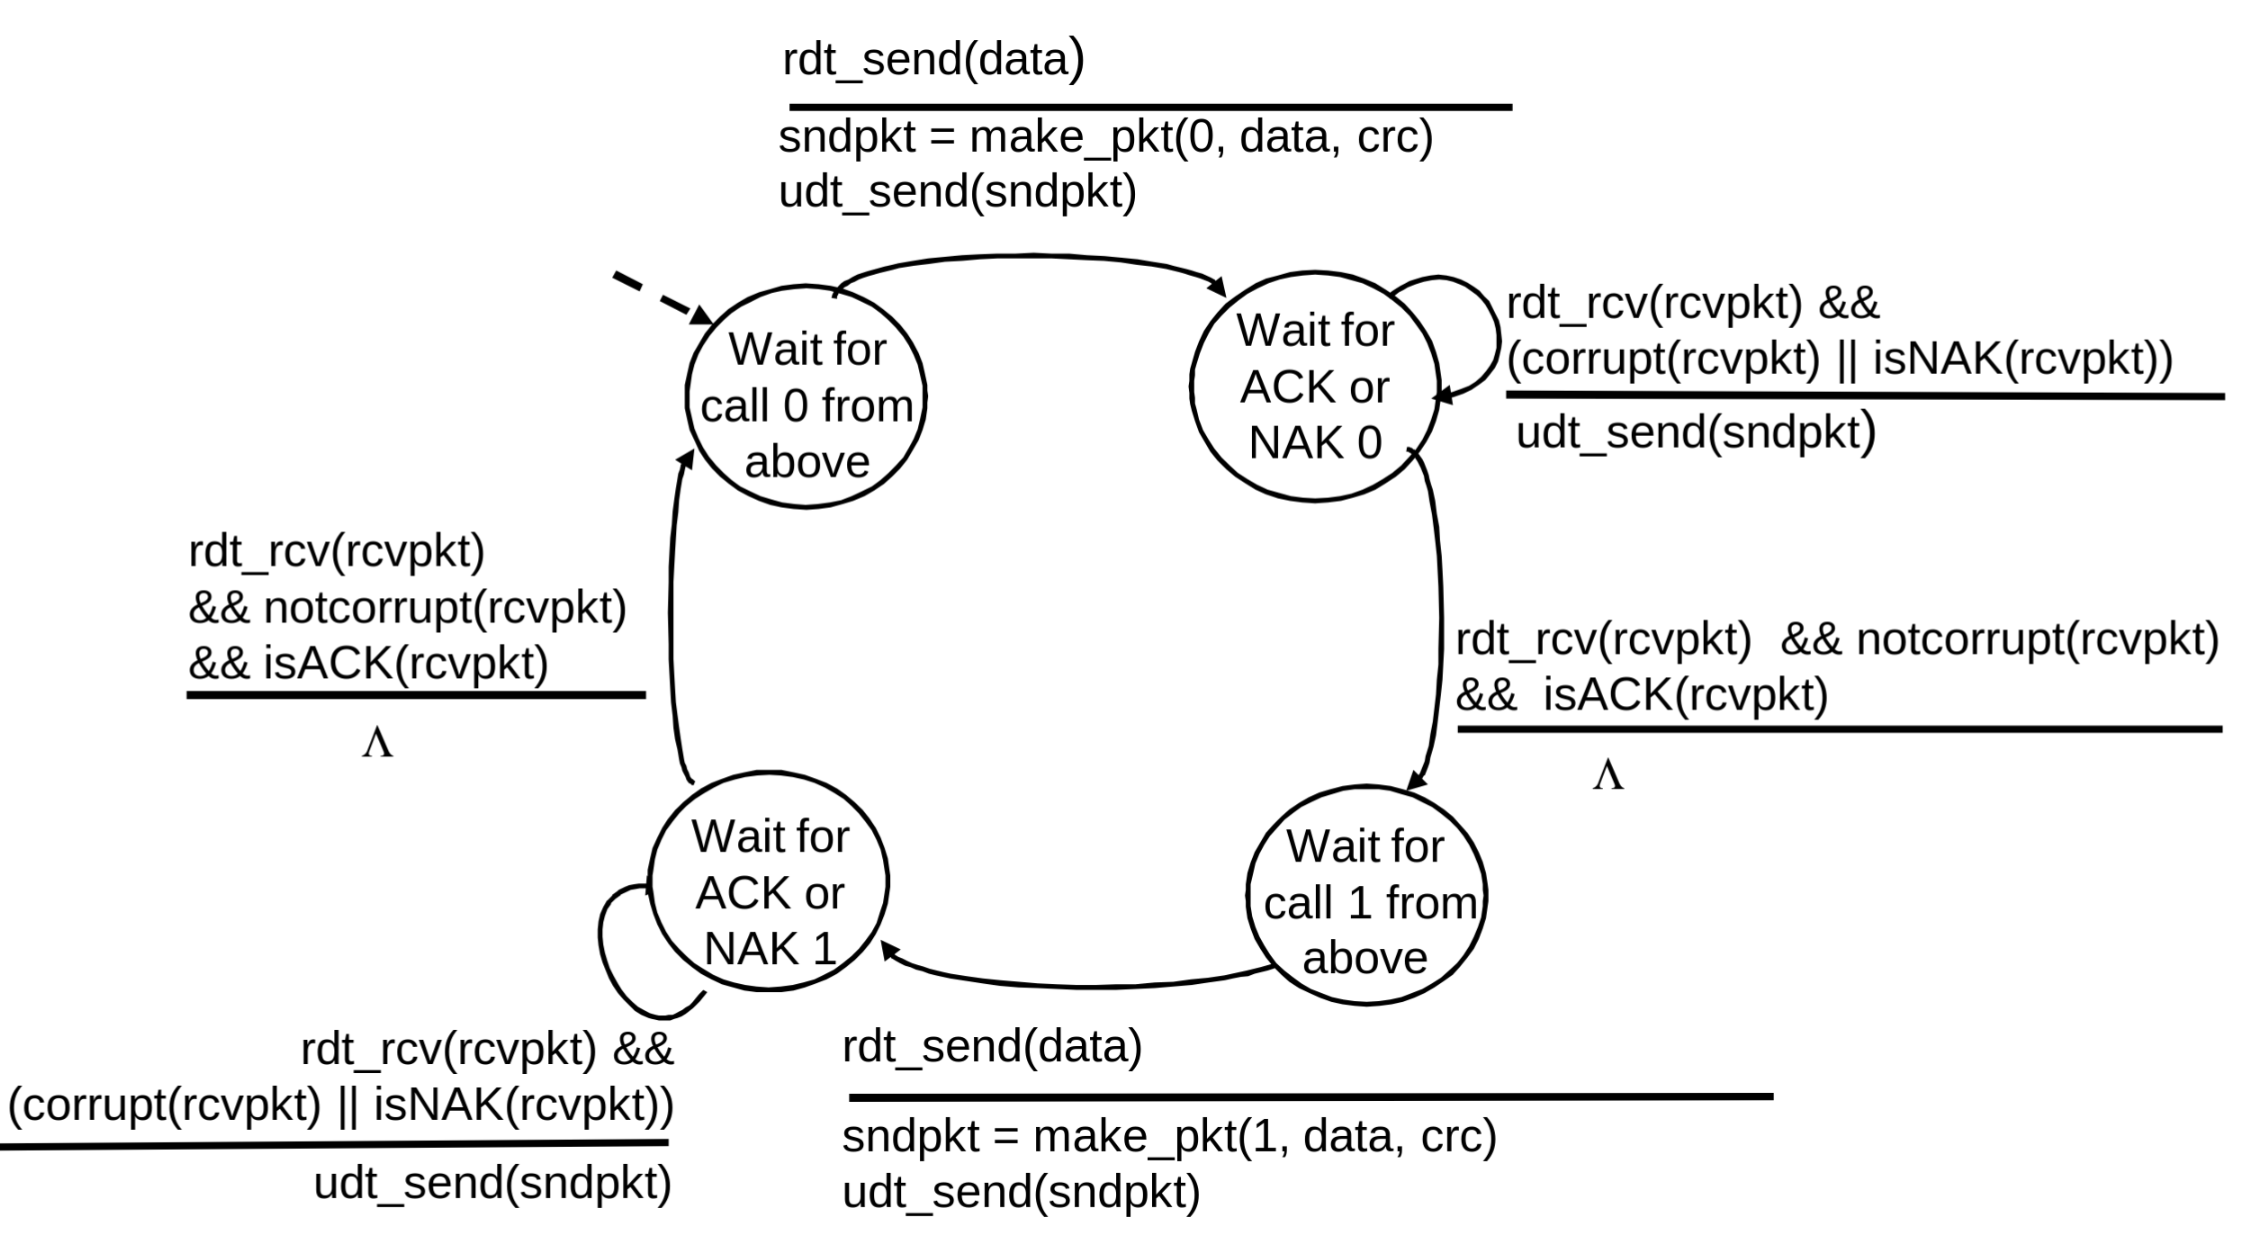
\includegraphics[scale=0.25]{../figures/rdt21fsm.png}
\end{center}

Quello che facciamo è:
\begin{itemize}
	\item Aspettare la chiamata dall'alto ed inviare il primo pacchetto (con numero di sequenza 0);
	\item Continuare ad inviare il pacchetto finche non si riceve un ACK non corrotto;
	\item Aspettare la chiamata dall'alto ed inviare il secondo pacchetto (con numero di sequenza 1);
	\item Di nuovo, continuare ad inviare il pacchetto finche non si riceve un ACK non corrotto.
\end{itemize}

Questo andamento si ripete in maniera ciclica.

\newpage

Il ricevitore potrà a questo punto eseguire il seguente automa:
\begin{center}
	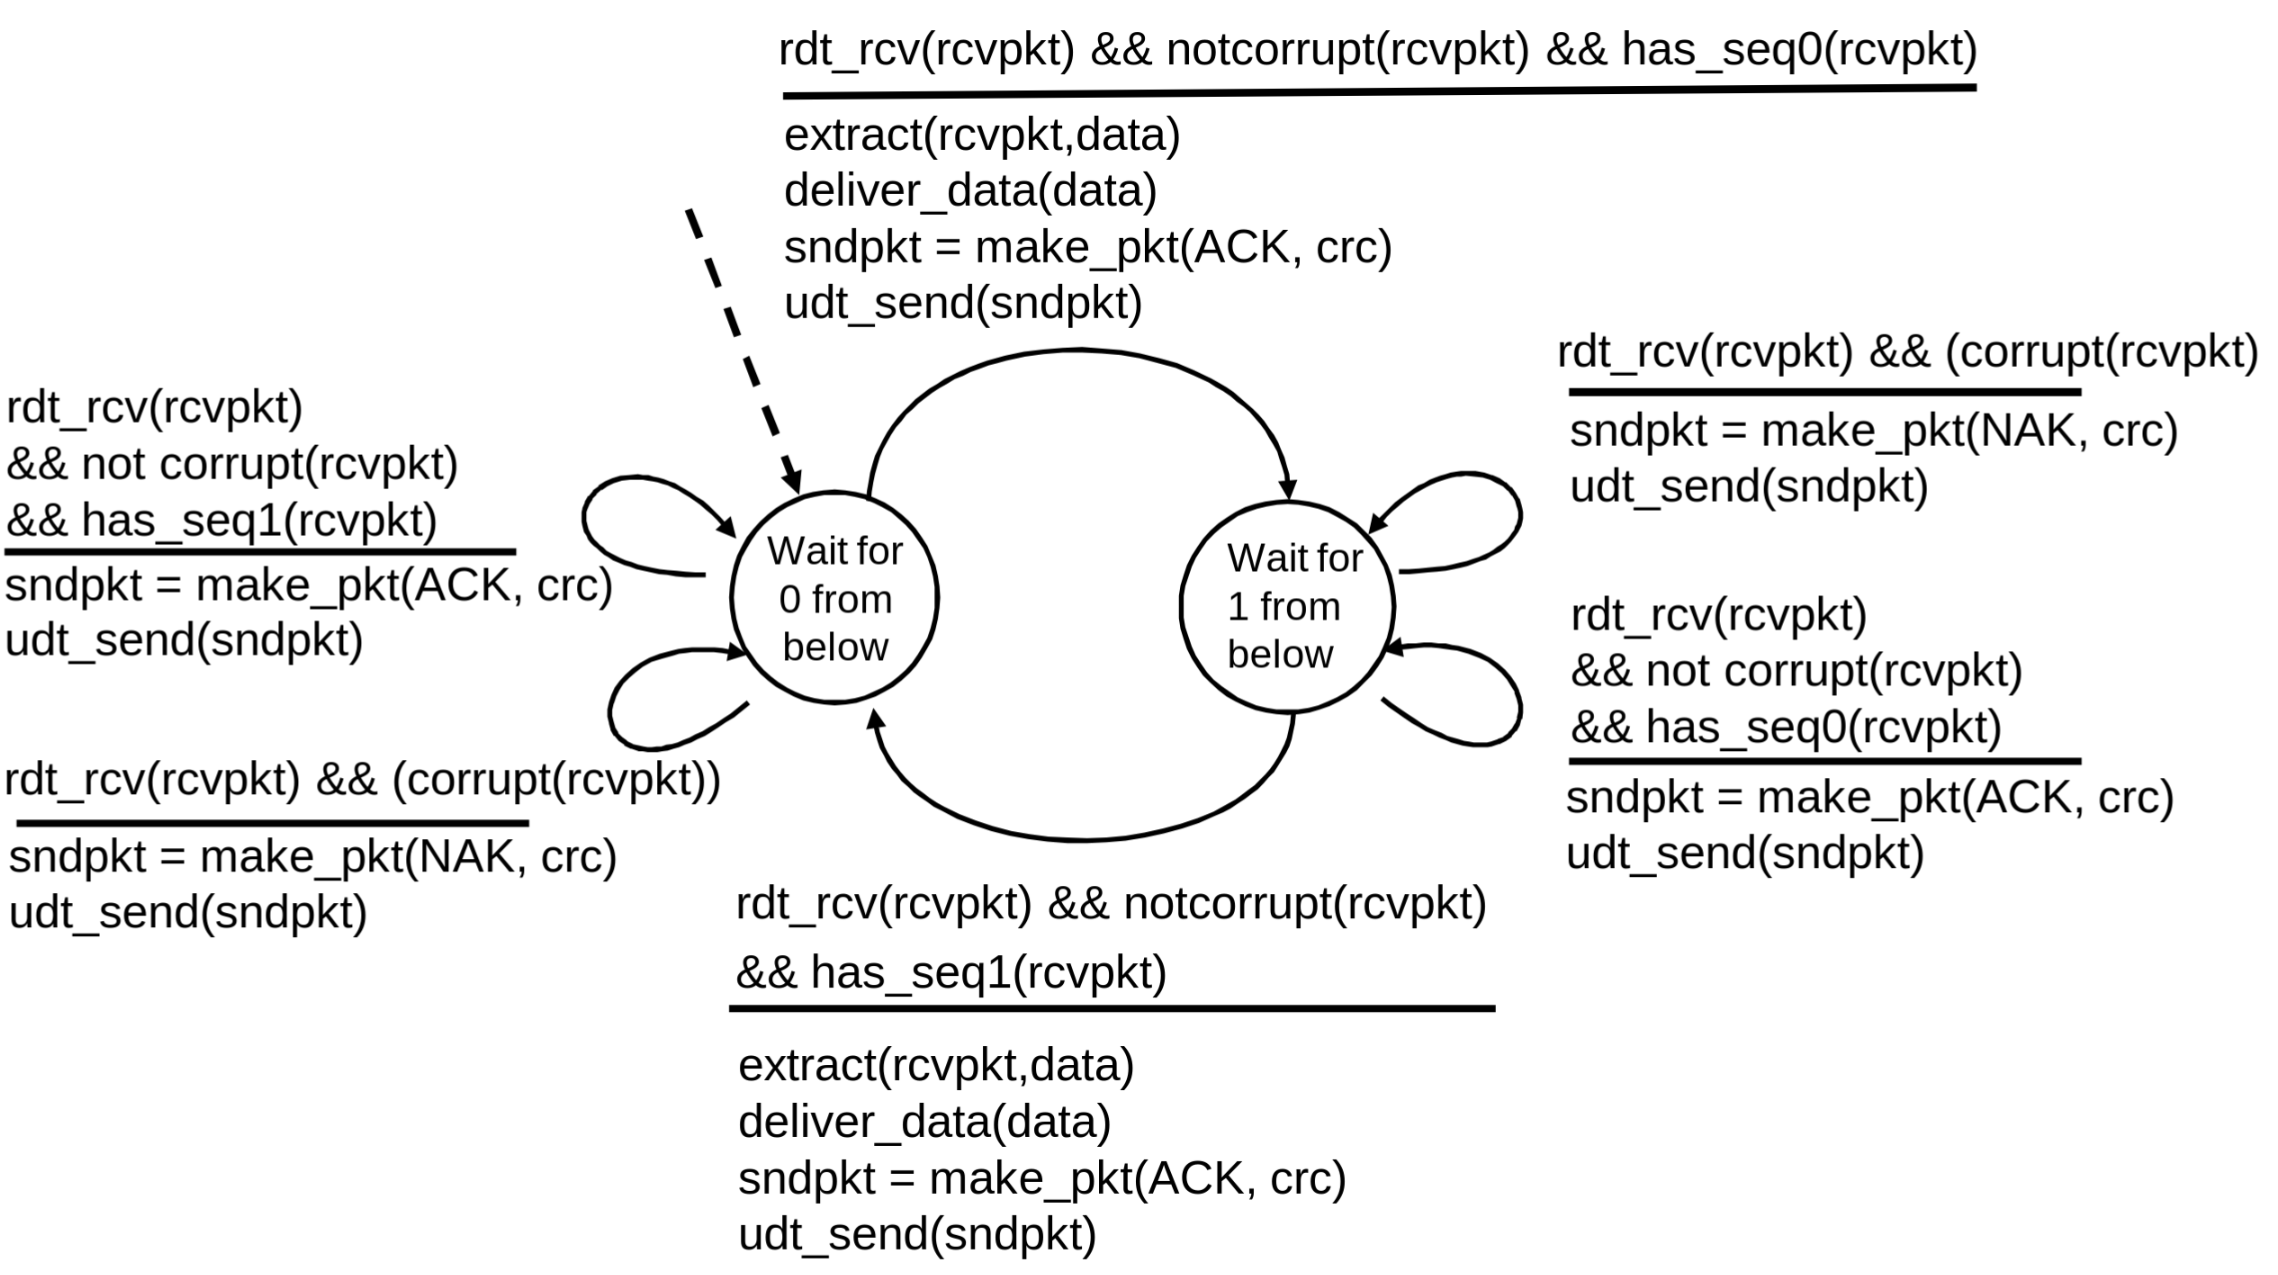
\includegraphics[scale=0.25]{../figures/rdt21fsm2.png}
\end{center}

In questo caso il flusso è:
\begin{itemize}
	\item Si aspetta per il primo pacchetto (dopo la chiamata dall'alto), si invia un pacchetto ACK nel caso questo arrivi integro e con numero di sequenza 0, NAK altrimenti;
	\item Si aspetta il secondo pacchetto, comportandoci in maniera analoga, ma verificando che il numero di sequenza sia 1.
\end{itemize}

\subsubsection{RDT 2.2}
Si può semplificare l'approccio sopra riportato guardando semplicemente agli ACK e ai numeri di sequenza: in questo caso il ricevitore deve solo inviare ACK per gli ultimi pacchetti ottenuti integri.
ACK per pacchetti già trasmessi verrano interpretati dal trasmettitore come avevamo interpretato i NAK fino ad ora.

\newpage
In questo caso le macchine a stati si modificano come segue:
\begin{center}
	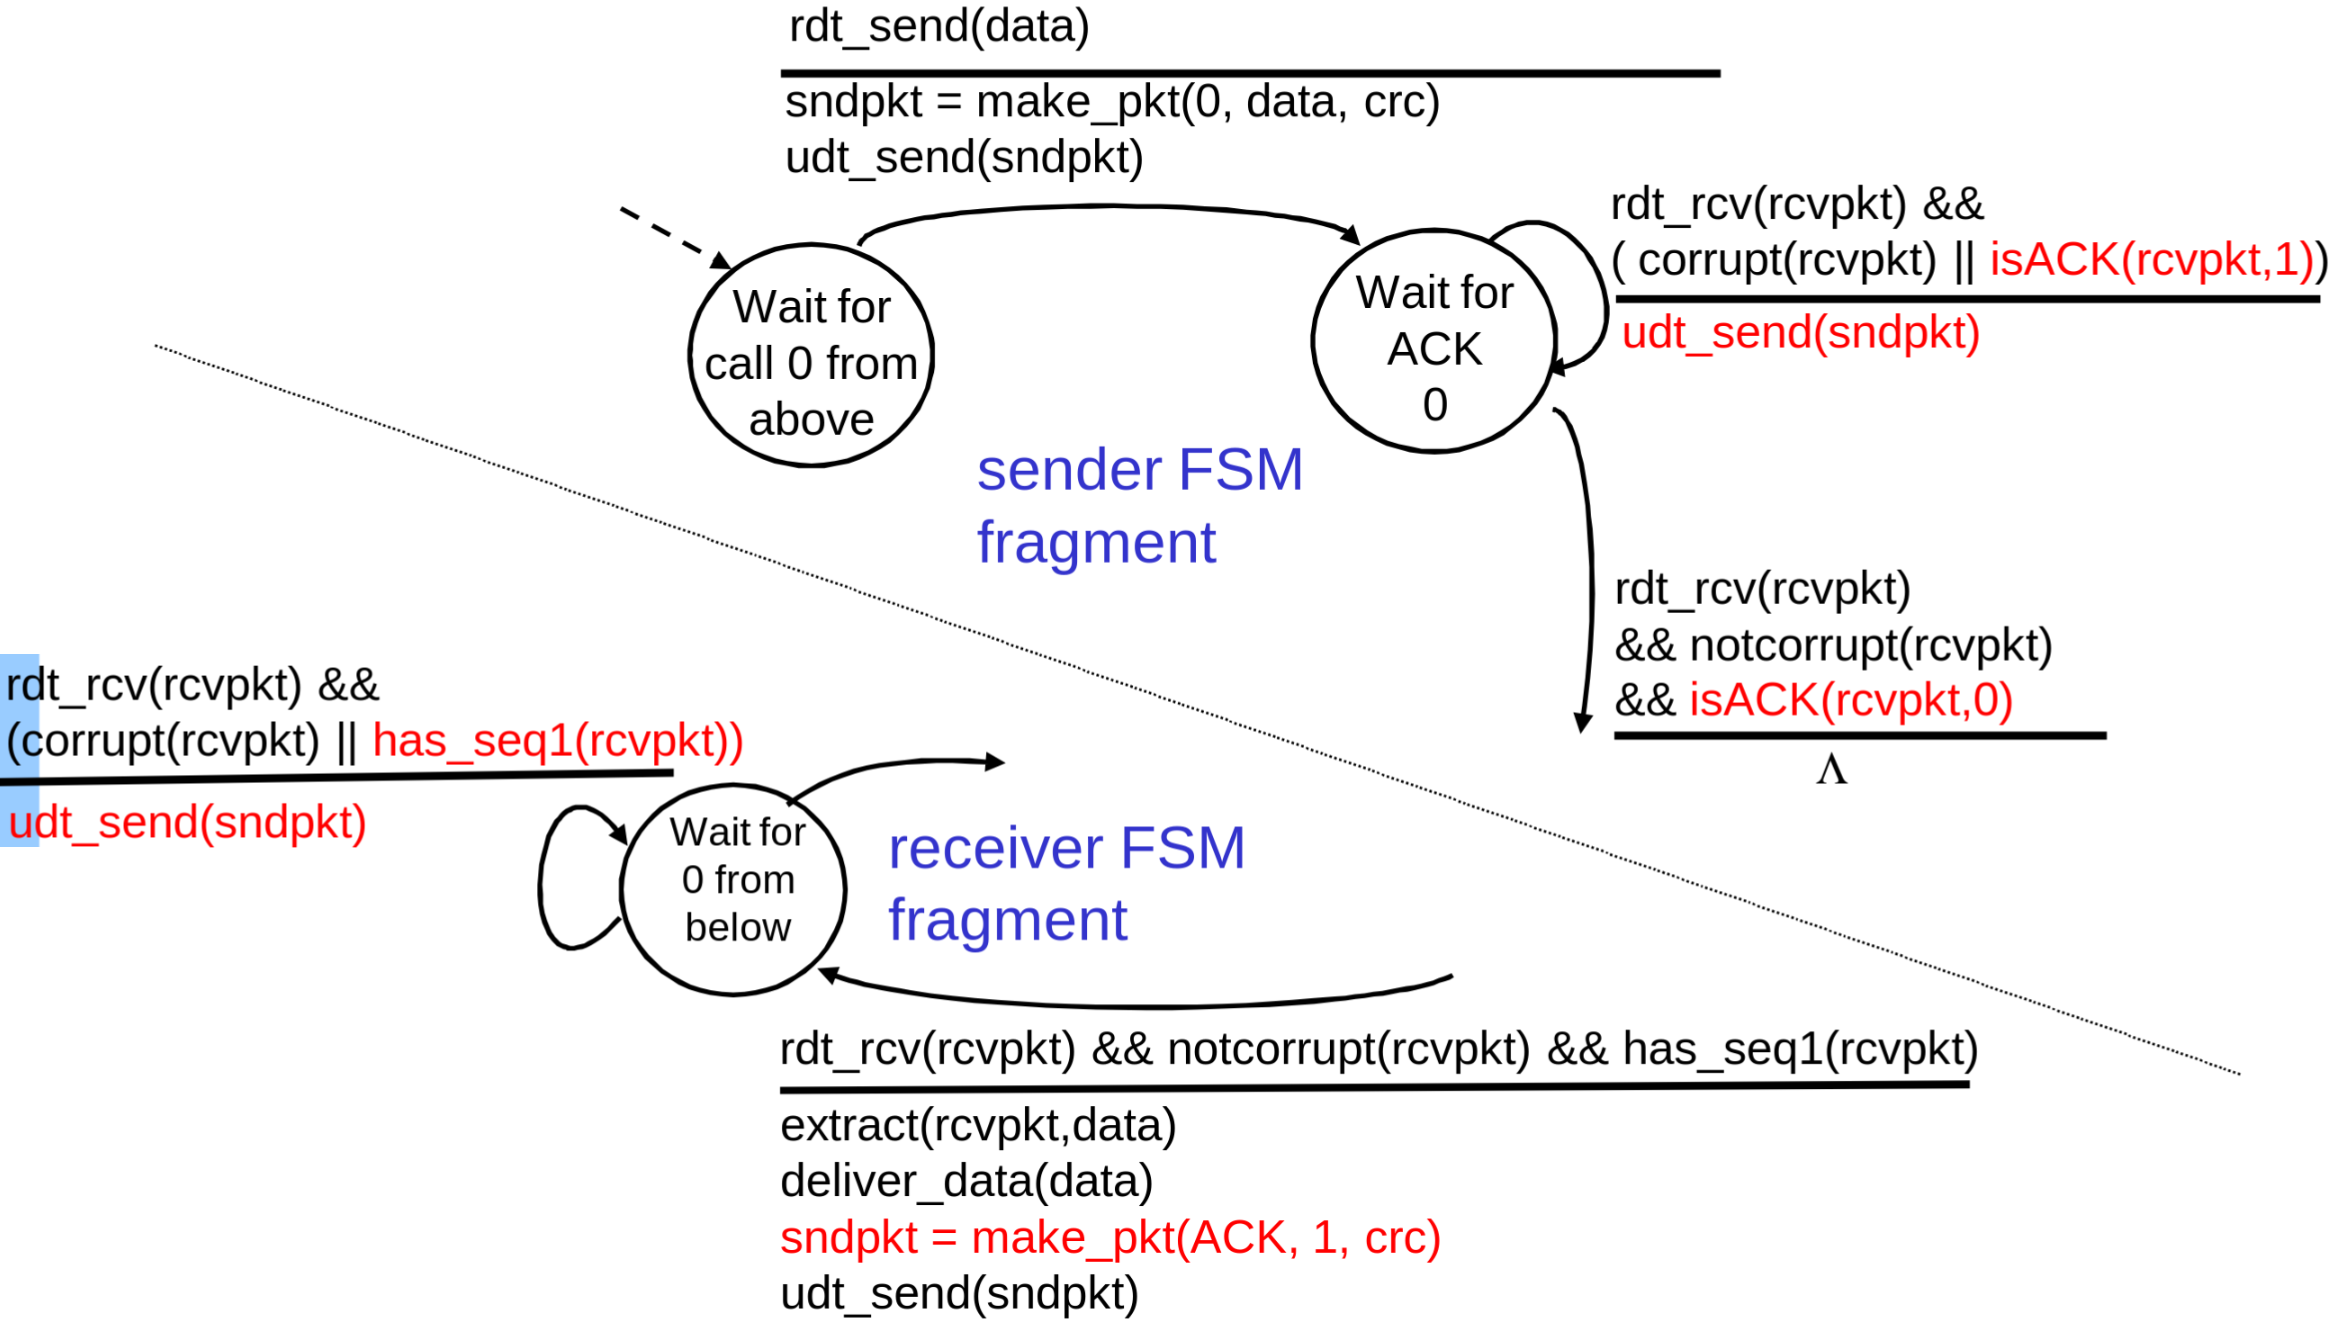
\includegraphics[scale=0.25]{../figures/rdt22fsm.png}
\end{center}

\subsection{RDT 3.0}
Facciamo una nuova assunzione sui canali: diciamo che il canale sottostante può anche \textit{perdere} (sia data che ACK), mentre prima poteva solo avere errori.

In questo caso potremo sfruttare checksum, numeri di sequenza, ACK e ritrasmissioni, ma non basterà completamente a risolvere il problema.

Un primo approccio potrebbe essere, lato tramsettitore, di aspettare un tempo ragionevole per l'arrivo dell'ACK da parte del ricevitore.
\textit{"Ragionevole"} può avere molti significati: assumiamo che il tempo sia tarato sul round-trip-time del link corrente.
Dopo che questo tempo passa, quindi, si procede col reinvio del pacchetto:
\begin{itemize}
	\item Se il pacchetto non era arrivato, il problema è risolto;
	\item Se il pacchetto era già arrivato e si era perso l'ACK, il ricevitore riceverà pacchetti duplicati: i numeri di sequenza risolvevano già questo prolema. Chiaramente, il ricevitore dovrà specificare il numero di sequenza del pacchetto per cui sta facendo ACK.
\end{itemize}

\newpage

La macchina a stati del trasmettitore con questo approccio è:
\begin{center}
	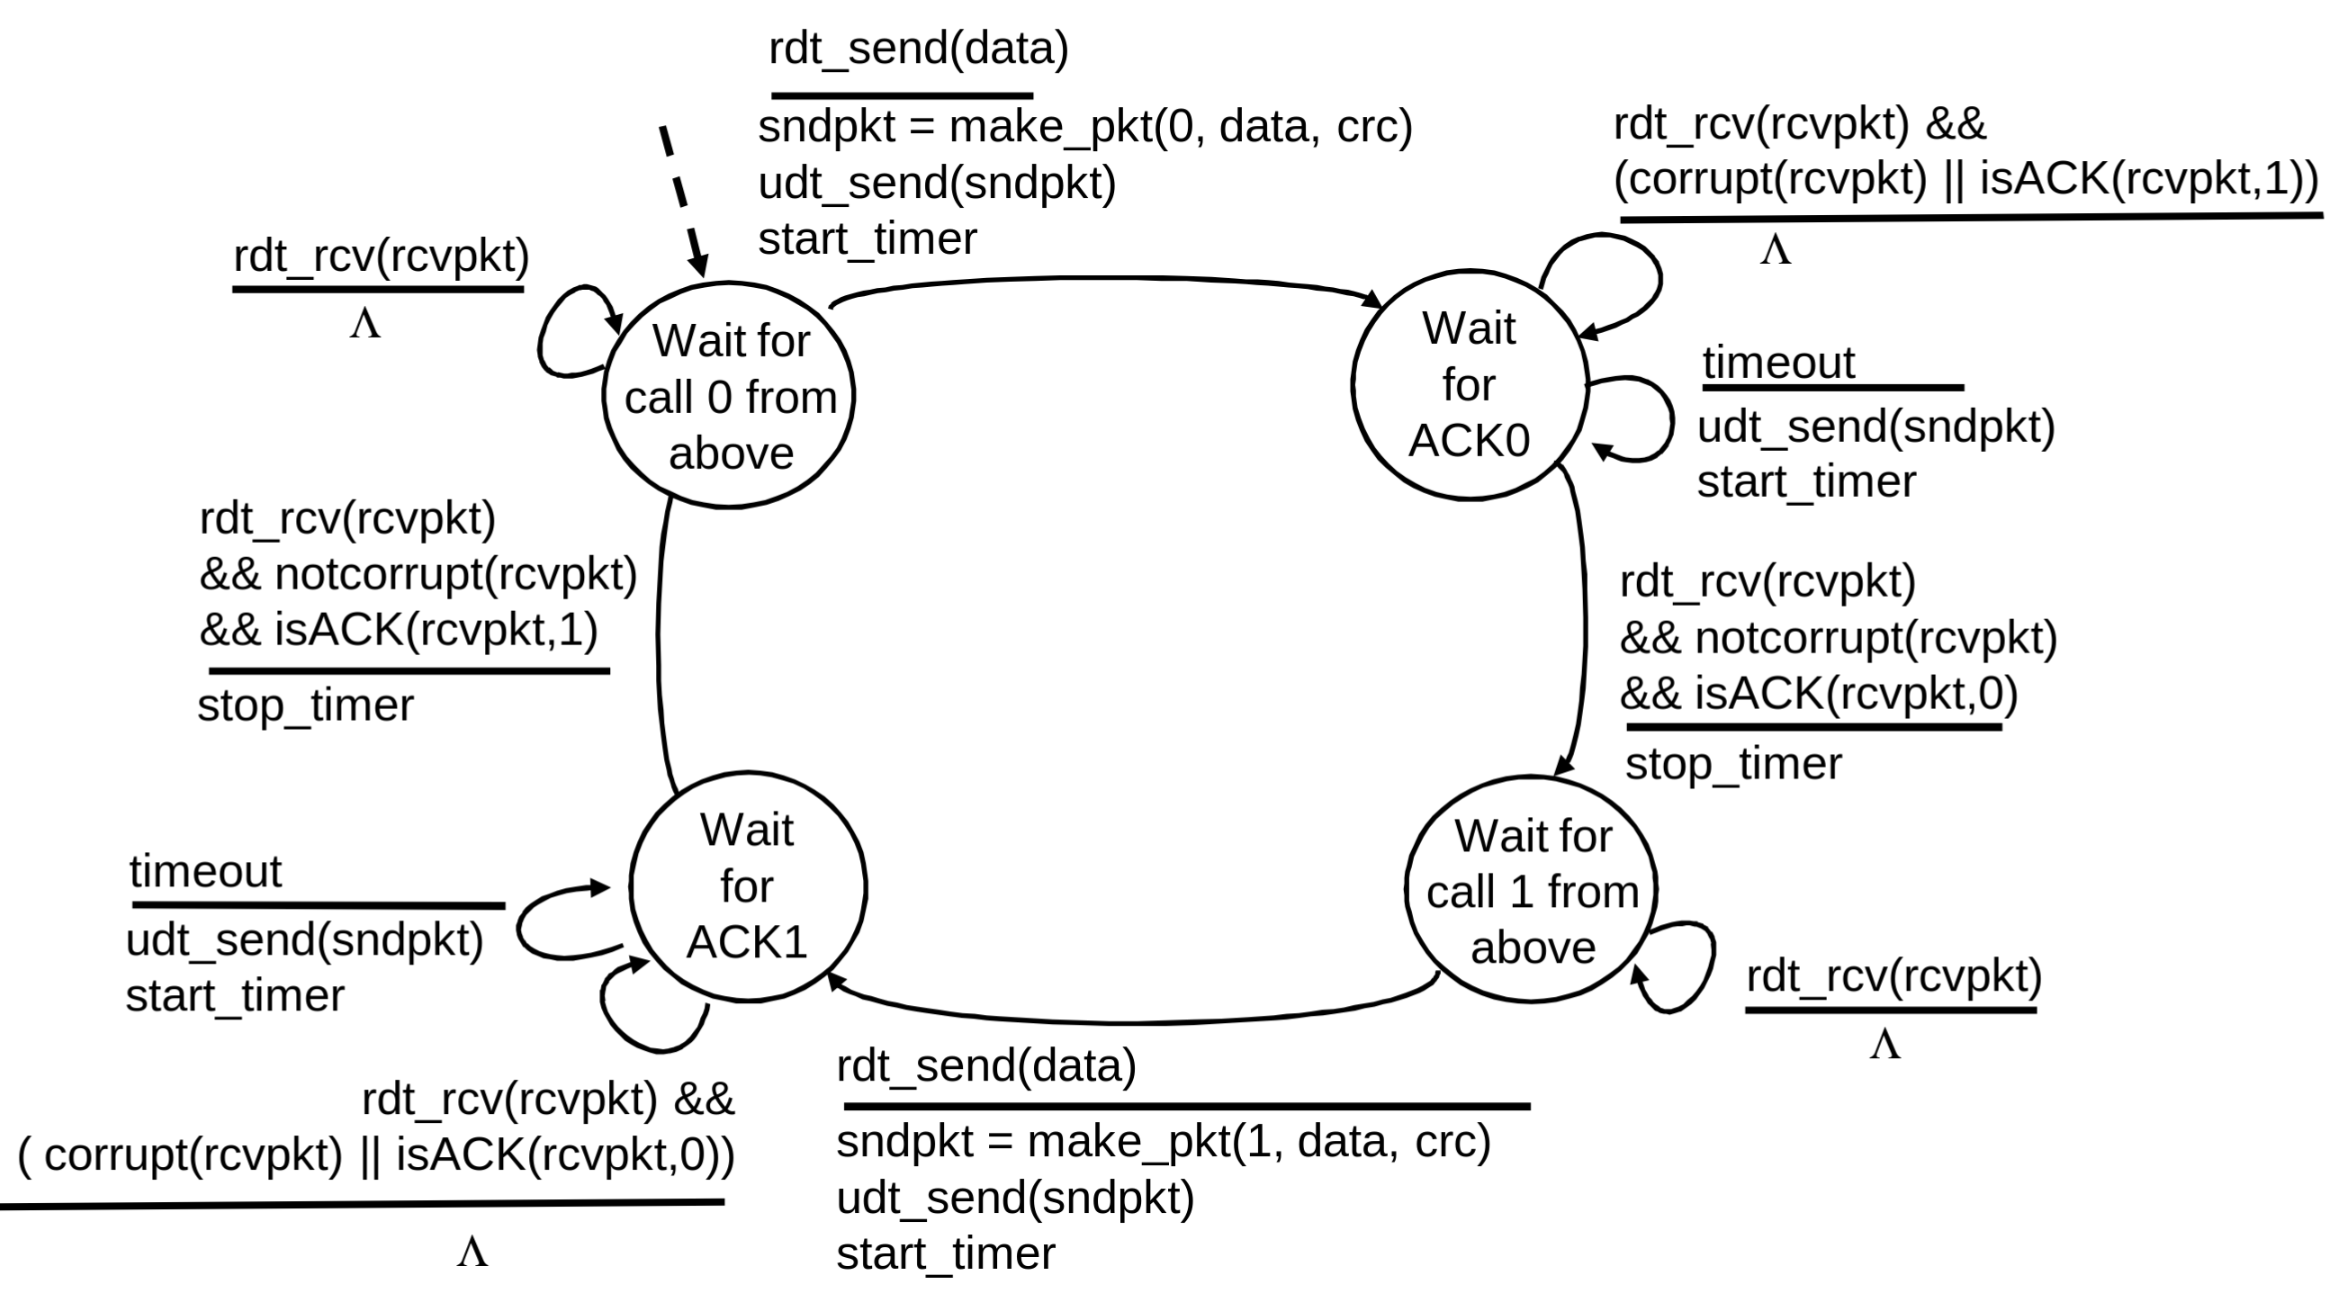
\includegraphics[scale=0.25]{../figures/rdt3fsm.png}
\end{center}

Ciò che facciamo è analogo a RDT 2.1, con la differenza che:
\begin{itemize}
	\item Quando inviamo il pacchetto, facciamo partire un timer;
	\item Se il timer fa timeout durante la fase di attesa per l'ACK, si reinvia il pacchetto al numero di sequenza corrente e si fa ripartire il timer.
\end{itemize}

Notiamo come si adotta un'approccio \textit{lazy} ai pacchetti ACK corrotti o per pacchetti con numero di sequenza sbagliato (quello che interpretavamo come NAK): in questo caso si ignorano e ci si affida al timeout (che prima o poi arriverà) per effettuare il reinvio.

Lato ricevitore, nulla cambia rispetto a RDT 2.2.

\subsubsection{Prestazioni di RDT 3.0}
Facciamo alcune note sulle \textbf{prestazioni} che riusciamo ad ottenere.

Sia $U_\text{sender}$ l'\textbf{utilizzazione tramsettitore}, cioè la frazione di tempo sul RTT usata dal trasmettitore in fase di invio effettivo del pacchetto.

Se assumiamo di avere un link da 1 Gbps, 15 ms di ritardo di propagazione e di dover trasmettere un pacchetto da 8000 bit.
Il tempo per trasmettere un pacchetto sul canale sarà allora circa:
$$
D_{\text{trans}} = \frac{L}{R} = \frac{8000}{1000} = 8 \, \text{ms}
$$

In condizioni ideali, quindi, avremo che dovremo inviare un pacchetto e aspettare un ACK (spedito in tempo trascurabile): questi sono due viaggi sul link (quindi un RTT dato dal due volte il ritardo di propagazione) e il tempo di trasmissione del pacchetto vero e proprio.
Si ha quindi:
$$
U_{\text{sender}} = \frac{ L/R }{ RTT + L/R } = \frac{0.0008}{30 + 0.0008} = 0.00027
$$

Cioè l'utilizzazione è terribile: del tempo che impieghiamo a trasmettere un pacchetto, meno dell'$0.001\%$ è effettivamente usato per trasmettere i dati che ci interessano!
Il problema è chiaramente che passiamo molto tempo ad \textit{aspettare}, quando potremmo avvantaggiarci con l'invio dei pacchetti successivi.

\subsection{Pipelining}
Il \textbf{pipelining} è un meccanismo attraverso il quale il trasmettitore può inviare più pacchetti in massa, senza aver ancora ricevuto l'ACK.
Lo poniamo come alternativa allo \textit{stop-and-wait} visto finora.

Riprendendo i conti della scorsa sezione, prendiamo ad esempio di inviare 3 pacchetti invece di 1 per ciclo di ACK. In questo caso si avrà:
$$
U_{\text{sender}} = \frac{ 3 L/R }{ RTT + L/R } = \frac{0.0024}{30 + 0.0008} = 0.00081
$$
che non è molto ma è già di più.

Chiaramente questo comporta delle complicazioni lato ricevitore: dovremmo prevedere la bufferizzazione dei pacchetti in entrata, e ingrandire il contatore del numero di sequenza (2 valori non basteranno più).

Trascurando quanto avviene lato ricevitore, una domanda interessante è \textit{quanti} pacchetti possiamo anticipare prima dell'ACK successivo: dovremmo riempire la finestra del $RTT$ con più tramissioni (ciascuna occupante tempo $\frac{L}{R}$), cioè inviare un numero di pacchetti al massimo pari a:
$$
N = \frac{RTT}{L / R}
$$

Approcci di questo tipo vengono detti a \textbf{sliding window} (\textit{"finestra scorrevole"}), in quanto prendono buffer scorrevoli sul blocco di pacchetti da inviare.

\subsubsection{Recupero errori in pipelining}
Abbiamo visto che, se vogliamo implementare un protocollo in pipelining, dobbiamo adoperare alcune soluzioni tecniche:
\begin{itemize}
	\item Buffering al trasmettitore dei pacchetti da inviare;
	\item Buffering al ricevitore dei pacchetti da ricevere, senza nessuna assicurazione che questi vengano ricevuti in ordine (serve il numero di sequenza);
	\item Un contatore per il numero di sequenza più grande al ricevitore.
\end{itemize}

Le specifiche di queste soluzioni vengono definite dal protocollo per il recupero dagli errori che adottiamo. 
Ne vederemo i 2 principali, che sono \textbf{go-back-N} e \textbf{selective-repeat}.

\subsubsection{Go-back-N}
In questo caso il trasmettitore mette fino a $N$ pacchetti senza ACK in pipeline.
Al ricevitore viene permesso solo di inviare ACK cumulativi: non effettua ACK se perde uno degli $N$ pacchetti.
Il trasmettitore mantiene quindi un timeout per gli ultimi $N$ pacchetti inviati: se il timer scade reinvia tutti gli $N$ pacchetti.

\par\smallskip

Lato implementativo si ha quindi che il trasmettitore spedisce fino a $N$ pacchetti consecutivi sulla pipeline.
Il ricevitore invia da parte sua ACK consecutivi al pacchetto con numero di sequenza più alto ricevuto fino a quel momento (se bufferizzare o meno i pacchetti che non combaciano col numero di sequenza aspettato è una scelta implementativa).

Quando il primo pacchetto della sequenza spedita viene ricevuto, il trasmettitore sposta in avanti la sua finestra e spedisce il successivo, spostandosi così lungo il blocco di pacchetti.

Se un pacchetto viene perso, il trasmettitore aspetta senza spostare la finestra: prima o poi scatterà il timeout del pacchetto perso e verrà reinviato.
Lato ricevitore, possiamo aspettarci che questo passerà lo stesso intervallo temporale a inviare ACK sempre sull'ultimo pacchetto valido (con numero di sequenza consecutivo) ricevuto, e che il trasmettitore abbia ignorato tale ACK in quanto ascolta solo l'ACK più grande ricevuto.

\subsubsection{Selective repeat}
In questo caso il trasmettitore invia $N$ pacchetti senza ACK in pipeline (come sopra).
La differenza è che il ricevitore invia ACK per ogni pacchetto: il trasmettitore deve quindi mantenere un timer per ogni pacchetto inviato, e nel caso questo timer faccia timeout inviare solo il pacchetto corrispondente.

Questo approccio è chiaramente più efficiente: si ritrasmettono solo i pacchetti persi, a costo di un'implementazione più costosa sia lato trasmettitore (dobbiamo mantenere più timer) che ricevitore (dobbiamo inviare ACK separati per ogni pacchetto).

Il caso in cui approcci come il go-back-N vengono comunque usati è quello di dispositivi \textit{constraining} (come quelli che si usano nell'IoT): questi hanno prestazioni meno soddisfacenti e quindi impongono di usare protocolli meno efficienti.

\end{document}

\end{document}